\section{Growth regimes: analytical results and equilibrium transitions}
\label{sec:numerical}

This section organizes the results around four economically distinct regimes. Each
case first states what follows analytically from the model and then presents an
equilibrium path that illustrates the result and the transition toward it. The
common equilibrium system, parameters, and numerical audit are presented once to
avoid repeating the same construction in every case.

Every path reported in this section solves the decentralized perfect-foresight
canonical system on its reported interval. The numerical solution imposes the household Euler equation, the
developer's research first-order and costate conditions, monopoly supply of AI
services, labor-market clearing, and the aggregate resource constraint. Earlier
experiments that fixed investment and automated-research spending as shares of
output are retained in the replication files as mechanism exercises, but they are
not used as evidence in the paper because they do not trace equilibrium paths.
The four cases are production complementarity, human-essential research at unit
production elasticity, substitutable research at unit production elasticity, and
production gross substitution. The figures quantify transition outcomes that the
analytical results do not sign. They do not convert necessary conditions or
conditional asymptotic characterizations into existence theorems.
The paths with $\sigma_{XL}\leq1$ approximate an infinite-horizon equilibrium by
moving the terminal date outward. The paths with $\sigma_{XL}>1$ are conditional
maximal equilibria on $[0,T^*)$, selected with the singular boundary derived in
conditional result~\ref{cond:high-sigma-singular-scaling}.

\subsection{Common equilibrium system and terminal conditions}

Capital and capability are predetermined. Aggregate consumption and the private
shadow value of capability are jump variables. Conditional on
$(K_t,A_t,N_t,q_t)$, the algorithm solves the monopoly condition
\eqref{eq:monopoly-ai-price}, labor-market clearing, and the two research
first-order conditions \eqref{eq:foc-human}--\eqref{eq:private-compute-foc}.
The four dynamic equations are
\begin{align}
    \frac{\dot K_t}{K_t}
    &=
    \frac{Y_t-C_t-\xi(U_t+M_t)}{K_t}-\delta,
    &
    \frac{\dot A_t}{A_t}
    &=\chi A_t^{\phi-1}E_t^\eta,
    \label{eq:equilibrium-numerical-states}\\
    \frac{\dot C_t}{C_t}
    &=n+r_t-\delta-\rho,
    &
    \frac{\dot q_t}{q_t}
    &=r_t-\delta-\phi\frac{\dot A_t}{A_t}
      -\frac{\pi^X_{A,t}}{q_t},
    \qquad
    \pi^X_{A,t}=\frac{\xi X_t}{A_t^2}.
    \label{eq:equilibrium-numerical-jumps}
\end{align}
The last two equations replace the exogenous saving and research-spending rules
used in the earlier mechanism exercises.

The model is solved as a boundary-value problem. Initial capital and capability are
fixed. The two terminal conditions are derived from the candidate asymptotic
equilibrium rather than imposed as arbitrary terminal stocks. When
$\sigma_{XL}<1$, they are
\begin{align}
    \frac{C_t}{Y_t}
    &\longrightarrow
    1-\frac{\alpha(n+\delta)}{\rho+\delta},
    &
    \frac{\pi^X_{A,t}}{q_t}
    &\longrightarrow
    \rho-(1-\eta)
    \frac{(1-\phi)n}{1-\phi+\eta}.
    \label{eq:low-sigma-equilibrium-terminal}
\end{align}
When $\sigma_{XL}=1$ and $\sigma_{HM}>1$, the terminal consumption share is given by
\eqref{eq:bg-consumption-share}, and the research first-order and costate
conditions give
\begin{equation}
    \frac{q_tA_t}{Y_t}
    \longrightarrow
    \frac{m_R^\infty}{\eta g_A^\infty}.
    \label{eq:cd-equilibrium-terminal}
\end{equation}
When $\sigma_{HM}=1$, the consumption target is obtained from
\eqref{eq:fully-cd-investment-share}--\eqref{eq:full-cd-research-resource-share},
and the shadow-value target replaces the denominator on the right-hand side with
$\eta\omega_M g_A^\infty$. Only the $\omega_M$ contribution of automated research
scales the machine first-order condition in that case.
The solver works with variables detrended by the analytical growth rates. The
complementarity path uses a 600-year terminal horizon. The two Cobb--Douglas
production paths use 2,000 years because convergence is slow. A separate horizon
test uses 400, 600, and 900 years for $\sigma_{XL}=0.75$ and 1,000, 1,500, and
2,000 years for each $\sigma_{XL}=1$ research technology. Across the three
sequences, initial log consumption changes by at most $1.1\times10^{-7}$ and the
initial log shadow value by at most $7.9\times10^{-6}$. The finite terminal date
therefore has no economically relevant effect on the reported initial jumps.

For $\sigma_{XL}>1$, Proposition~\ref{prop:gross-substitution-no-steady-state}
rules out the finite-rate, positive-capability-growth terminal condition used in the
other two regimes. We
instead use the postulated singular scaling in conditional
result~\ref{cond:high-sigma-singular-scaling}. Let
$z_t\equiv Y_t/K_t$ and choose a large terminal value $\bar z$. Calendar time to
that boundary is an endogenous parameter. In addition to the two initial stocks,
the boundary-value problem imposes
\begin{equation}
    z_T=\bar z,
    \qquad
    \frac{C_T}{Y_T}=\bar c,
    \qquad
    \frac{q_TA_T}{K_T}=\frac{d_U}{\eta\alpha}.
    \label{eq:high-sigma-numerical-boundary}
\end{equation}
We then raise $\bar z$ and retain a path only if its initial jump variables and the
implied singularity date stabilize. The boundary sequences are $\bar z=20,50$ for
$\sigma_{XL}=1.35$ and 1.50 and $\bar z=20,50,100$ for $\sigma_{XL}=2$. This
free-boundary method does not impose a growth rate or an arbitrary acceleration
cutoff.

\subsection{Common parameters and numerical validation}

Table~\ref{tab:equilibrium-numerical-parameters} reports the common parameters and
initial stocks. The exercises are illustrative and are not a calibration. In
    particular, the scale parameter $\chi$ is a normalization retained across all
production elasticities; the solution does not renormalize it to equalize initial
capability growth.

\begin{table}[H]
    \centering
    \caption{Parameters for the equilibrium transitions}
    \label{tab:equilibrium-numerical-parameters}
    \begin{tabular}{lcl}
        \toprule
        Object & Value & Interpretation \\
        \midrule
        $\alpha$ & 0.33 & capital elasticity \\
        $(\omega_L,\omega_X)$ & $(0.80,0.20)$ & production CES weights \\
        $n$ & 1.20\% & population growth \\
        $\delta$ & 5.00\% & capital depreciation \\
        $\rho$ & 4.00\% & discount rate \\
        $(\phi,\eta)$ & $(0.65,0.45)$ & ideas-production elasticities \\
        $\sigma_{HM}$ & 1.00 or 2.00 & research substitution elasticity \\
        $(\omega_H,\omega_M)$ & $(0.65,0.35)$ & research CES weights \\
        $\xi$ & 1.00 & standardized compute cost \\
        $\chi$ & 0.09839 & research-productivity normalization \\
        $(K_0,A_0,N_0)$ & $(2.509,1,1)$ & initial stocks \\
        $\sigma_{XL}$ & $0.75$, $1.00$, $1.35$, $1.50$, or $2.00$ & production elasticity \\
        \bottomrule
    \end{tabular}
\end{table}

For $\sigma_{HM}=2$, the common parameters imply
$D_{\mathrm{CD}}=0.3106$ and $D_{\mathrm{AI}}=0.2375$. Both feedback
denominators are positive. The numerical comparison across values of
$\sigma_{XL}$ therefore holds the reduced research-feedback classification in its
stable region. In particular, the acceleration reported for $\sigma_{XL}>1$ is not
generated by setting $D_{\mathrm{CD}}\leq0$ or $D_{\mathrm{AI}}\leq0$; it identifies
the separate production-side mechanism.

The numerical design does not form the full Cartesian product of all parameter
values. Table~\ref{tab:targeted-configurations} selects five configurations within
the four regimes analyzed below. Four configurations have canonical equilibrium
paths. The strong-feedback configuration in Case III is an analytical stress test:
without an economically justified terminal condition, a reduced singular path
would not constitute an equilibrium simulation.

\begin{table}[H]
    \centering
    \caption{Targeted parameter configurations}
    \label{tab:targeted-configurations}
    \resizebox{\textwidth}{!}{%
    \begin{tabular}{clcccc}
        \toprule
        Case & Configuration & $\sigma_{XL}$ & $\sigma_{HM}$ & Feedback region & Numerical status \\
        \midrule
        I & Labor bottleneck & 0.75 & 2.00 & $D_{\mathrm{AI}}>0$ & canonical equilibrium \\
        II & Human-essential research & 1.00 & 1.00 & $D_{\mathrm{CD}}>0$ & canonical equilibrium \\
        III & Gradual research automation & 1.00 & 2.00 & $D_{\mathrm{AI}}>0$ & canonical equilibrium \\
        III & Strong research feedback & 1.00 & 2.00 & $D_{\mathrm{CD}}>0>D_{\mathrm{AI}}$ & analytical stress test \\
        IV & Production-side acceleration & 1.35 & 2.00 & $D_{\mathrm{AI}}>0$ & free-boundary equilibrium \\
        \bottomrule
    \end{tabular}}
    \begin{minipage}{0.96\textwidth}
    \footnotesize\emph{Notes:} The canonical equilibrium path reported for each of
    Cases I--IV holds all other parameters and the initial stocks in
    Table~\ref{tab:equilibrium-numerical-parameters} fixed. In the Case III stress
    test, setting $\phi=0.90$ while retaining $\eta=0.45$ gives
    $D_{\mathrm{CD}}=0.0606$ and $D_{\mathrm{AI}}=-0.0125$. The additional
    $\sigma_{XL}=1.50$ and 2.00 paths are timing-robustness exercises for
    Case IV, not separate economic regimes.
    \end{minipage}
\end{table}

Table~\ref{tab:equilibrium-system-audit} audits the six equilibrium paths against the complete
canonical system in \eqref{eq:equilibrium-trajectory-system}--
\eqref{eq:equilibrium-optimality-system}. The algebraic column includes
the two CES technologies, $X=AU$, factor pricing, final-firm zero profit, the
household budget, and the developer's profit identity. The dynamic column compares
the derivative of each collocation polynomial with the right-hand side of the laws
of motion for $K$, $A$, $C$, and $q$. The static column covers resource and labor
clearing and the monopoly and research first-order conditions. The endpoint column
checks the terminal restrictions used by each boundary-value problem. The final column is
the smallest value of the normalized second-order margin in
\eqref{eq:eqsys-monopoly-soc}; a positive number verifies a strict maximum.

\begin{table}[H]
    \centering
    \caption{Audit of the numerical equilibrium system}
    \label{tab:equilibrium-system-audit}
    \resizebox{\textwidth}{!}{%
    \begin{tabular}{ccccccc}
        \toprule
        $\sigma_{XL}$ & $\sigma_{HM}$ & algebraic residual & dynamic residual
        & static residual & endpoint residual & monopoly margin \\
        \midrule
        0.75 & 2.00 & $6.5\times10^{-12}$ & $7.5\times10^{-8}$
             & $1.4\times10^{-9}$ & $5.3\times10^{-9}$ & 0.0788 \\
        1.00 & 2.00 & $1.8\times10^{-13}$ & $1.5\times10^{-5}$
             & $1.4\times10^{-11}$ & $1.4\times10^{-15}$ & 0.1160 \\
        1.00 & 1.00 & $2.3\times10^{-13}$ & $1.5\times10^{-5}$
             & $3.5\times10^{-13}$ & $1.5\times10^{-13}$ & 0.1160 \\
        1.35 & 2.00 & $5.9\times10^{-11}$ & $8.4\times10^{-6}$
             & $1.4\times10^{-10}$ & $7.0\times10^{-13}$ & 0.1986 \\
        1.50 & 2.00 & $4.1\times10^{-11}$ & $2.1\times10^{-6}$
             & $9.9\times10^{-11}$ & $1.7\times10^{-13}$ & 0.2211 \\
        2.00 & 2.00 & $8.9\times10^{-11}$ & $1.7\times10^{-5}$
             & $2.0\times10^{-10}$ & $5.9\times10^{-13}$ & 0.2178 \\
        \bottomrule
    \end{tabular}}
    \begin{minipage}{0.96\textwidth}
    \footnotesize\emph{Notes:} Each residual is the largest absolute residual in
    its group over the reported path. Endpoint conditions are imposed and therefore
    check implementation rather than economics. The monopoly margin is a lower bound, so its
    sign rather than its absolute size is the relevant diagnostic. Consumption,
    investment, production labor, human research, and $q$ remain positive in all
    six solutions.
    \end{minipage}
\end{table}

\begin{table}[htbp]
    \centering
    \caption{Endpoints of the equilibrium transitions}
    \label{tab:equilibrium-transition-endpoints}
    \resizebox{\textwidth}{!}{%
    \begin{tabular}{cccccccccc}
        \toprule
        $\sigma_{XL}$ & $\sigma_{HM}$ & Year & $g_{A,0}$ & $g_{A,T}$ & $g_{Y/N,T}$
        & $g_{C/N,T}$ & $s^X_T$ & $s^M_T$ & $C_T/Y_T$ \\
        \midrule
        0.75 & 2.00 & 600 & 1.027\% & 0.703\% & 0.0056\% & 0.0250\%
             & 33.64\% & 12.23\% & 77.27\% \\
        1.00 & 1.00 & 2,000 & 0.377\% & 1.738\% & 0.435\% & 0.435\%
             & 20.00\% & 35.00\% & 74.85\% \\
        1.00 & 2.00 & 2,000 & 0.445\% & 2.271\% & 0.568\% & 0.568\%
             & 20.00\% & 99.93\% & 74.35\% \\
        \bottomrule
    \end{tabular}}
    \begin{minipage}{0.96\textwidth}
    \footnotesize\emph{Notes:} The analytical capability-growth limits are
    0.675 percent when $\sigma_{XL}=0.75$, 1.738 percent when both elasticities
    equal one, and 2.274 percent when $\sigma_{XL}=1$ and $\sigma_{HM}=2$.
    The small difference between output- and
    consumption-per-capita growth at the complementarity endpoint reflects the
    remaining transition, not a violation of household optimality.
    \end{minipage}
\end{table}

\subsection{Case I: production complementarity, $\sigma_{XL}<1$}
\label{sec:case-production-complements}

\subsubsection{Analytical characterization}

Conditional result~\ref{cond:nonunit-ces-steady-states} establishes a necessary
property of any interior finite-rate limit with positive capability growth. When
$\sigma_{XL}<1$, labor is the asymptotic bottleneck in final production. Output,
capital, and consumption per capita must therefore have zero limiting growth,
whereas capability can continue to grow at
$\eta n/(1-\phi+\eta)$. Along an optimizing path, inference and automated
research spending also become negligible relative to output, as shown in
\eqref{eq:low-sigma-declining-research-shares}. These restrictions characterize a
possible limit; they do not prove that an equilibrium converges to it.

\subsubsection{Equilibrium transition}

Unless stated otherwise, the $\sigma_{XL}=1$ path in the common figures uses
$\sigma_{HM}=2$ and serves as a reference for Case III. The human-essential path is
shown separately in Case II.

Figure~\ref{fig:equilibrium-levels} reports the first 600 years. Along the
complementarity path, output, consumption, and capital per capita initially fall and
then recover toward finite levels, while capability continues to increase. The
unit-elasticity path is included in the figure only as a common reference and is
analyzed in Cases II and III.

\begin{figure}[H]
    \centering
    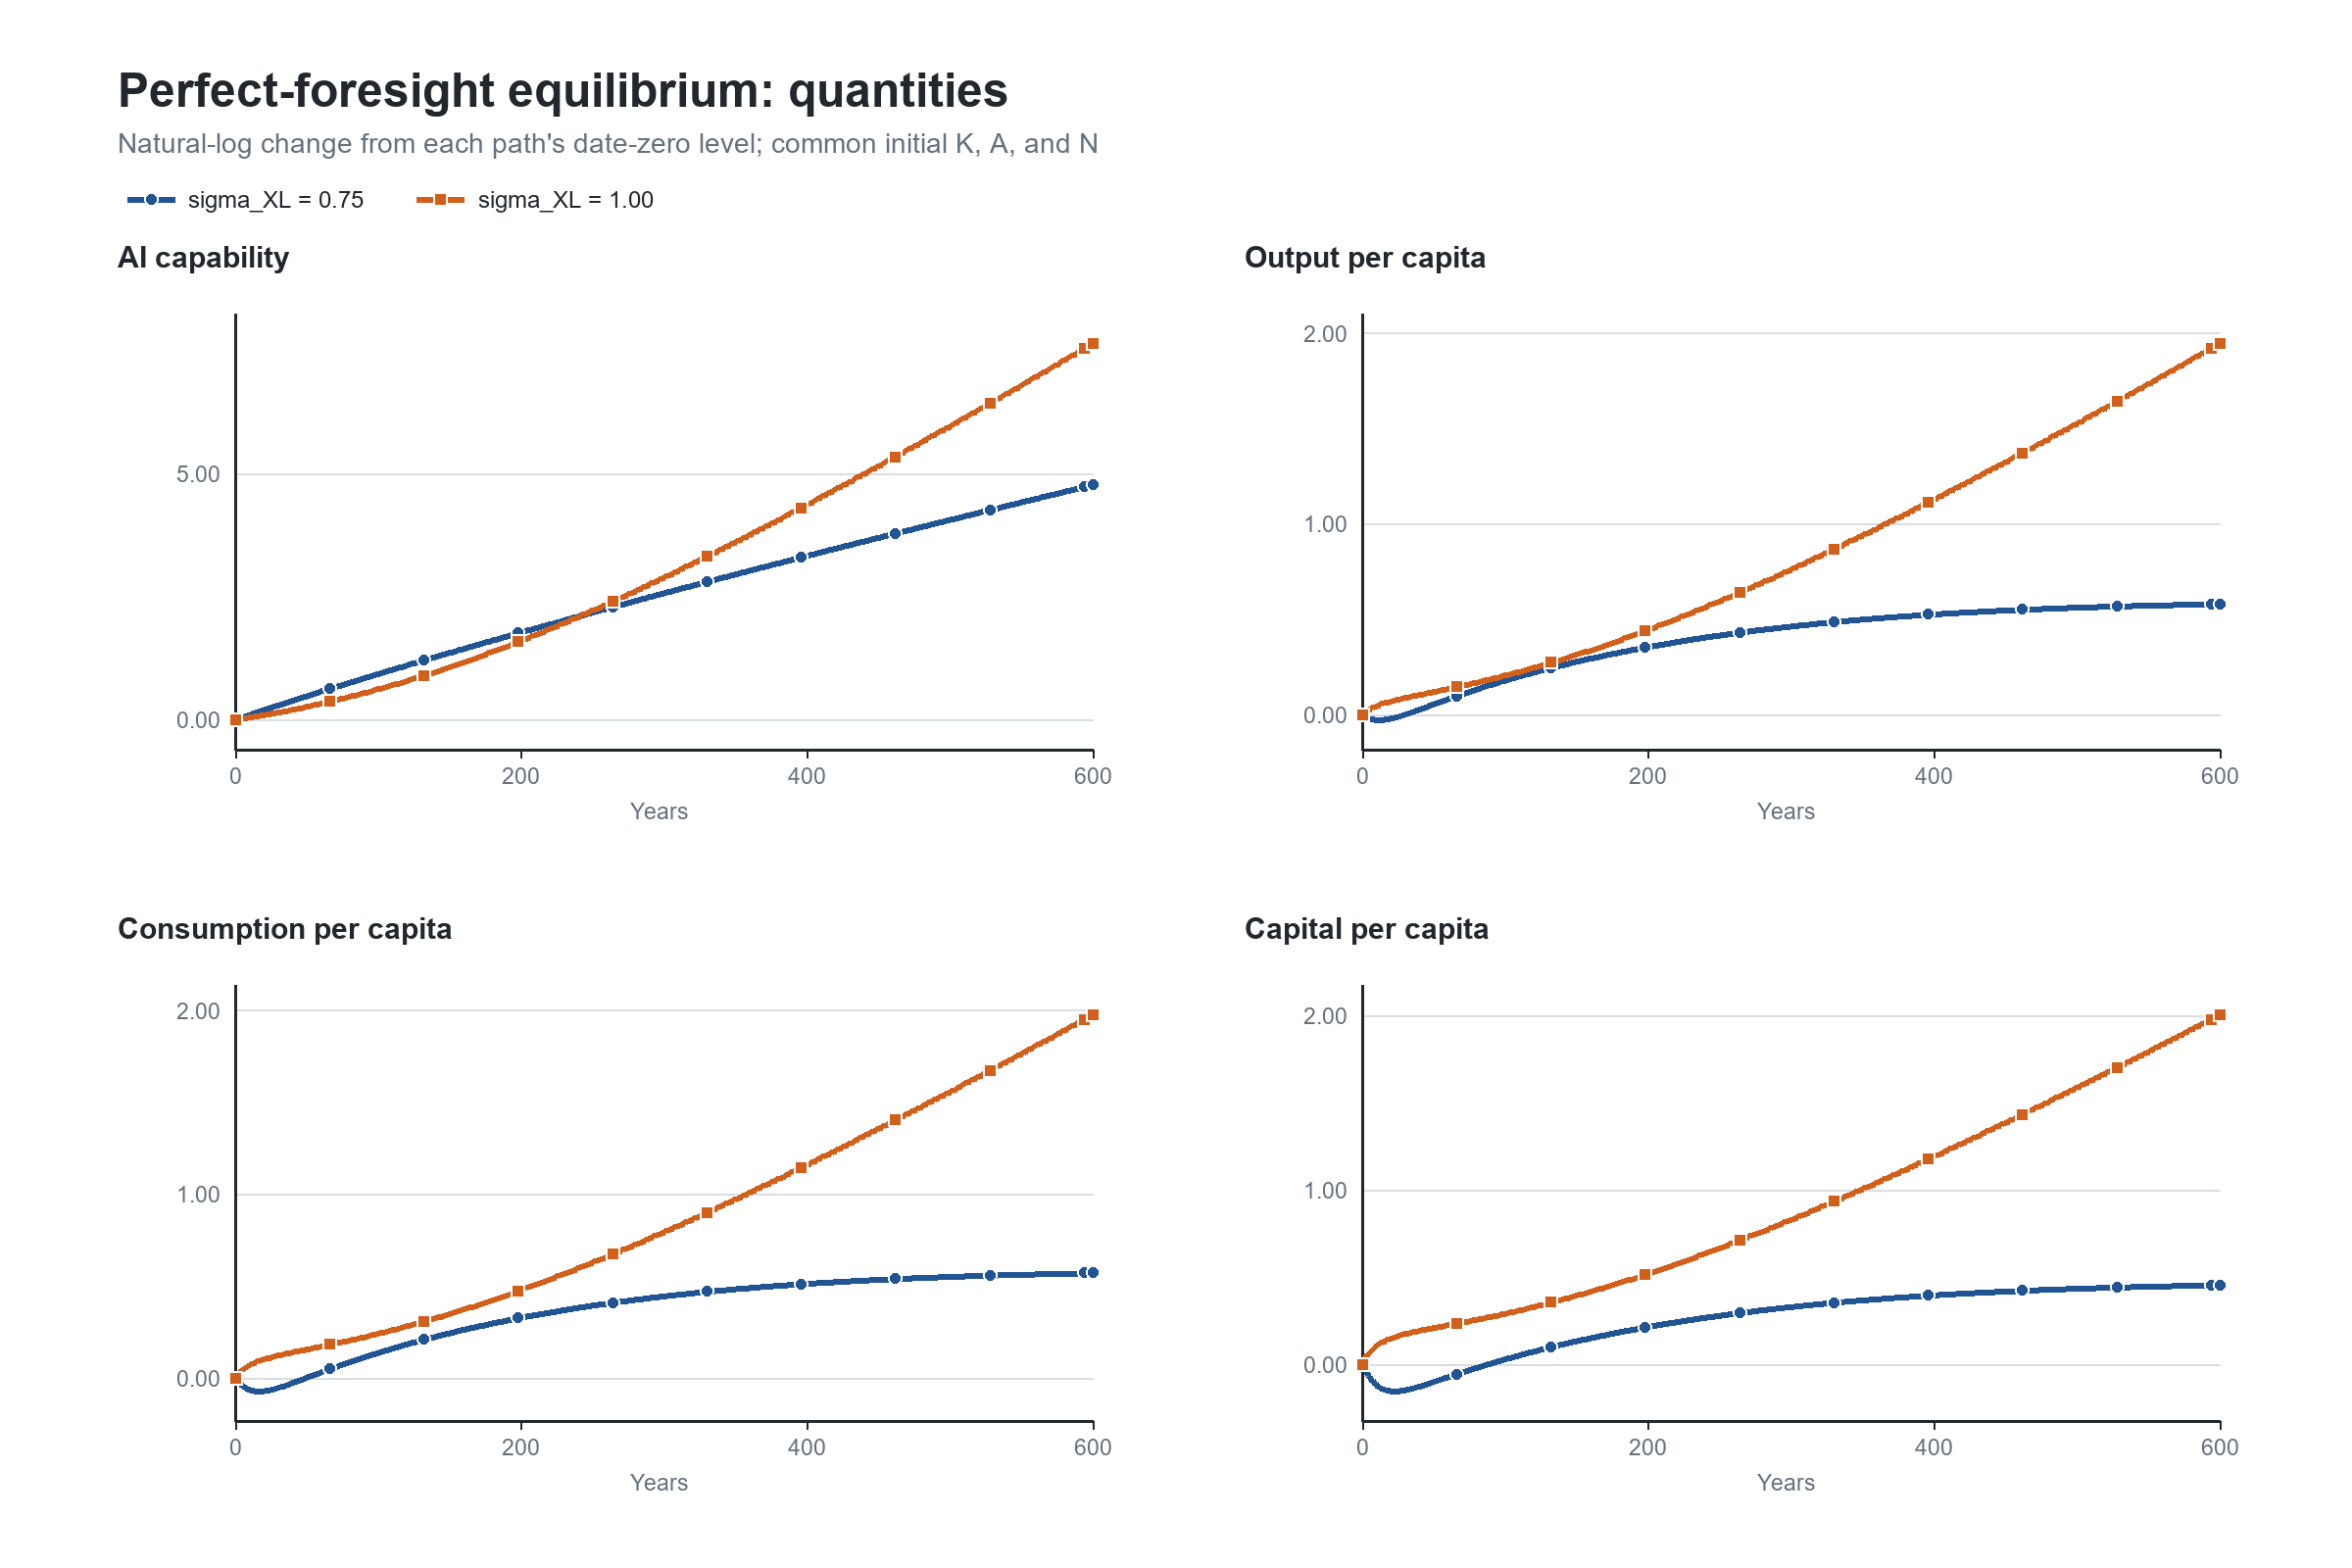
\includegraphics[width=\textwidth]{figures/equilibrium_levels.png}
    \caption{Equilibrium quantities. Each panel reports the natural-log change
    relative to the path's date-zero value. Both paths satisfy the
    household and developer optimality conditions.}
    \label{fig:equilibrium-levels}
\end{figure}

Figure~\ref{fig:equilibrium-growth-rates} makes the complementarity result precise.
When $\sigma_{XL}=0.75$, output-per-capita growth is not zero at every date. It is
negative initially, becomes positive during the recovery, and then converges toward
zero. By year 600 it is 0.0056 percent. Capability growth remains positive and is
close to its analytical limit of 0.675 percent. The experiment therefore
illustrates the production bottleneck characterized in conditional
result~\ref{cond:nonunit-ces-steady-states}; it does not prove convergence or
existence of the required equilibrium limit.

The net return satisfies the Euler equation. Along the complementarity path it
converges to 4 percent, the household discount rate, because consumption per capita
eventually stops growing.

\begin{figure}[H]
    \centering
    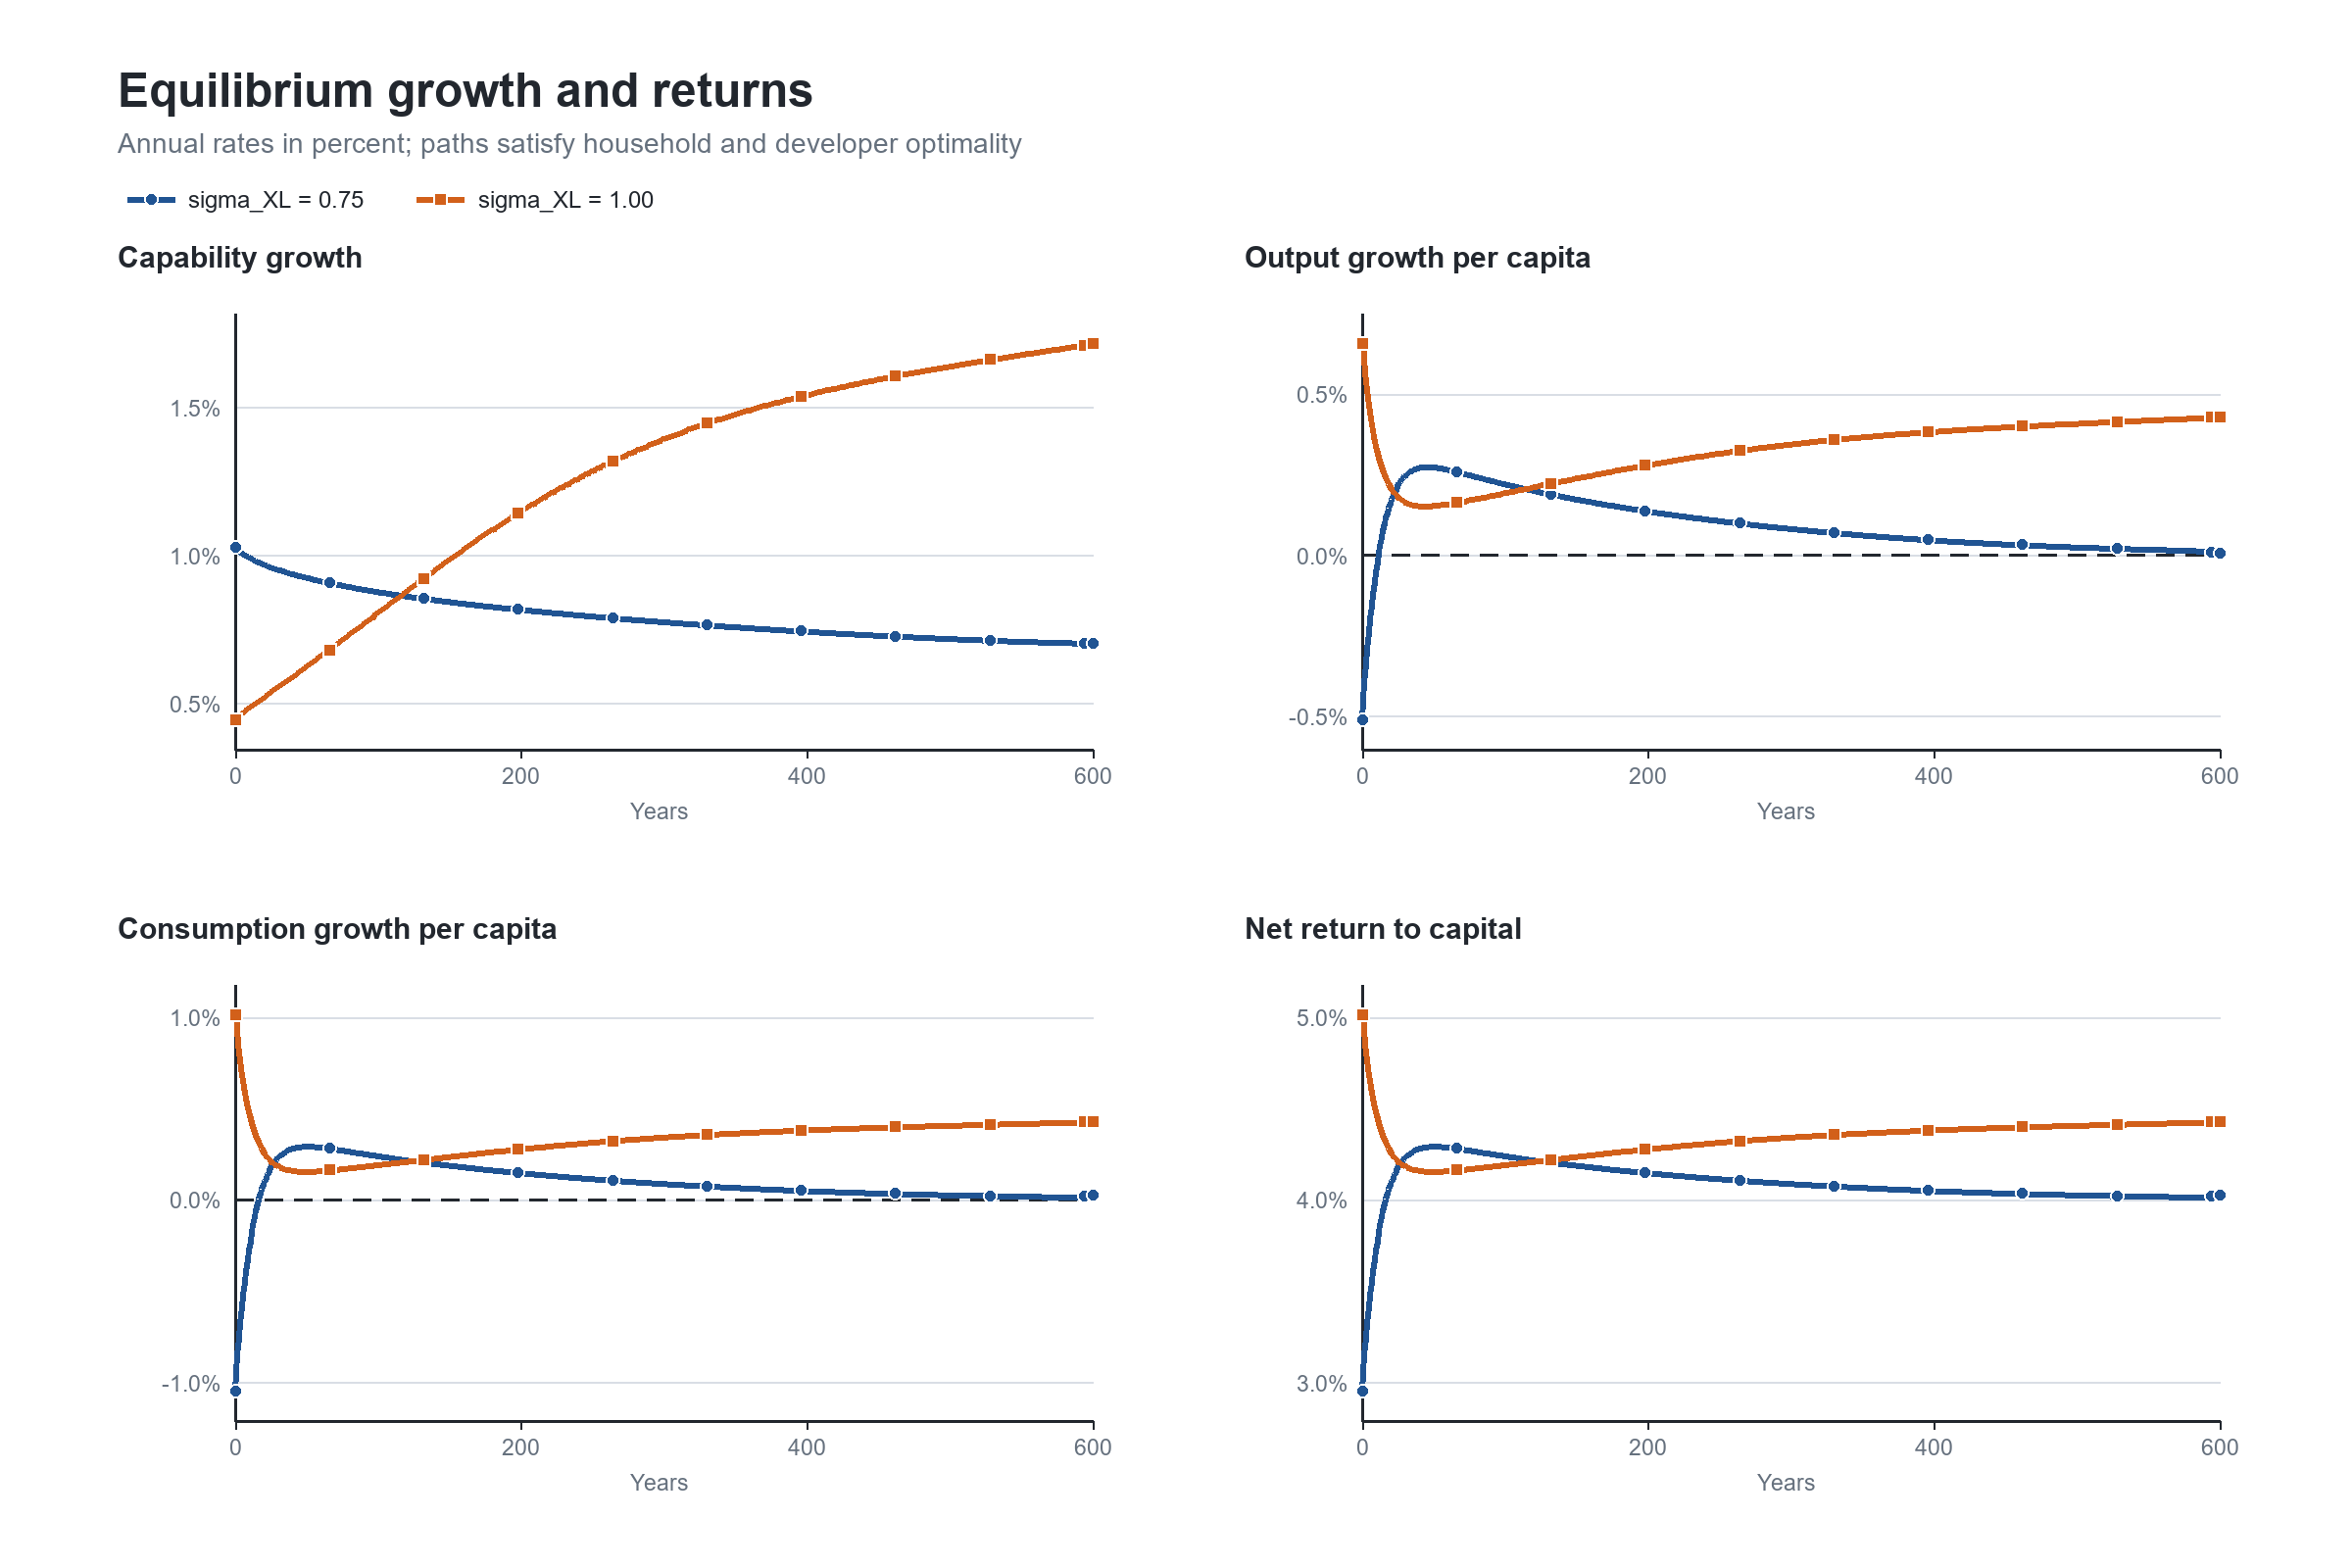
\includegraphics[width=\textwidth]{figures/equilibrium_growth_rates.png}
    \caption{Equilibrium growth rates and the net return to capital. Rates are
    annual. The dashed line marks zero per-capita growth.}
    \label{fig:equilibrium-growth-rates}
\end{figure}

\subsection{Case II: human-essential research at unit production elasticity}
\label{sec:case-human-essential}

\subsubsection{Analytical characterization}

Set $\sigma_{XL}=\sigma_{HM}=1$. The automated contribution to effective research
is then the constant $\omega_M$, so human research remains essential even when
$H/M$ tends to zero. Equations~\eqref{eq:full-cd-ga}--
\eqref{eq:fully-cd-growth-rates} give the candidate constant growth rates. Positive
finite capability growth requires $D_{\mathrm{CD}}>0$, and an interior allocation
also requires the consumption-feasibility condition
\eqref{eq:fully-cd-consumption-feasibility}. On that path, $H/N$ is constant,
$H/M$ declines, and output per capita grows at
$(\omega_X/\omega_L)\eta n/D_{\mathrm{CD}}$. The positivity of
$D_{\mathrm{CD}}$ alone is therefore not an existence theorem.

\subsubsection{Equilibrium transition}

Figure~\ref{fig:equilibrium-research-technology-comparison} holds the production
elasticity and every common parameter fixed and changes only $\sigma_{HM}$. When
$\sigma_{HM}=1$, the automated contribution to effective research remains equal to
$\omega_M=35$ percent. Capability growth converges to 1.738 percent and output and
consumption per capita grow at 0.435 percent. Human research employment converges
to 0.497 percent of the population. The ratio $H/M$ nevertheless converges to zero:
human input becomes small relative to automated input without ceasing to be
essential for effective research. The $\sigma_{HM}=2$ path in the same figure is
analyzed in Case III.

\begin{figure}[H]
    \centering
    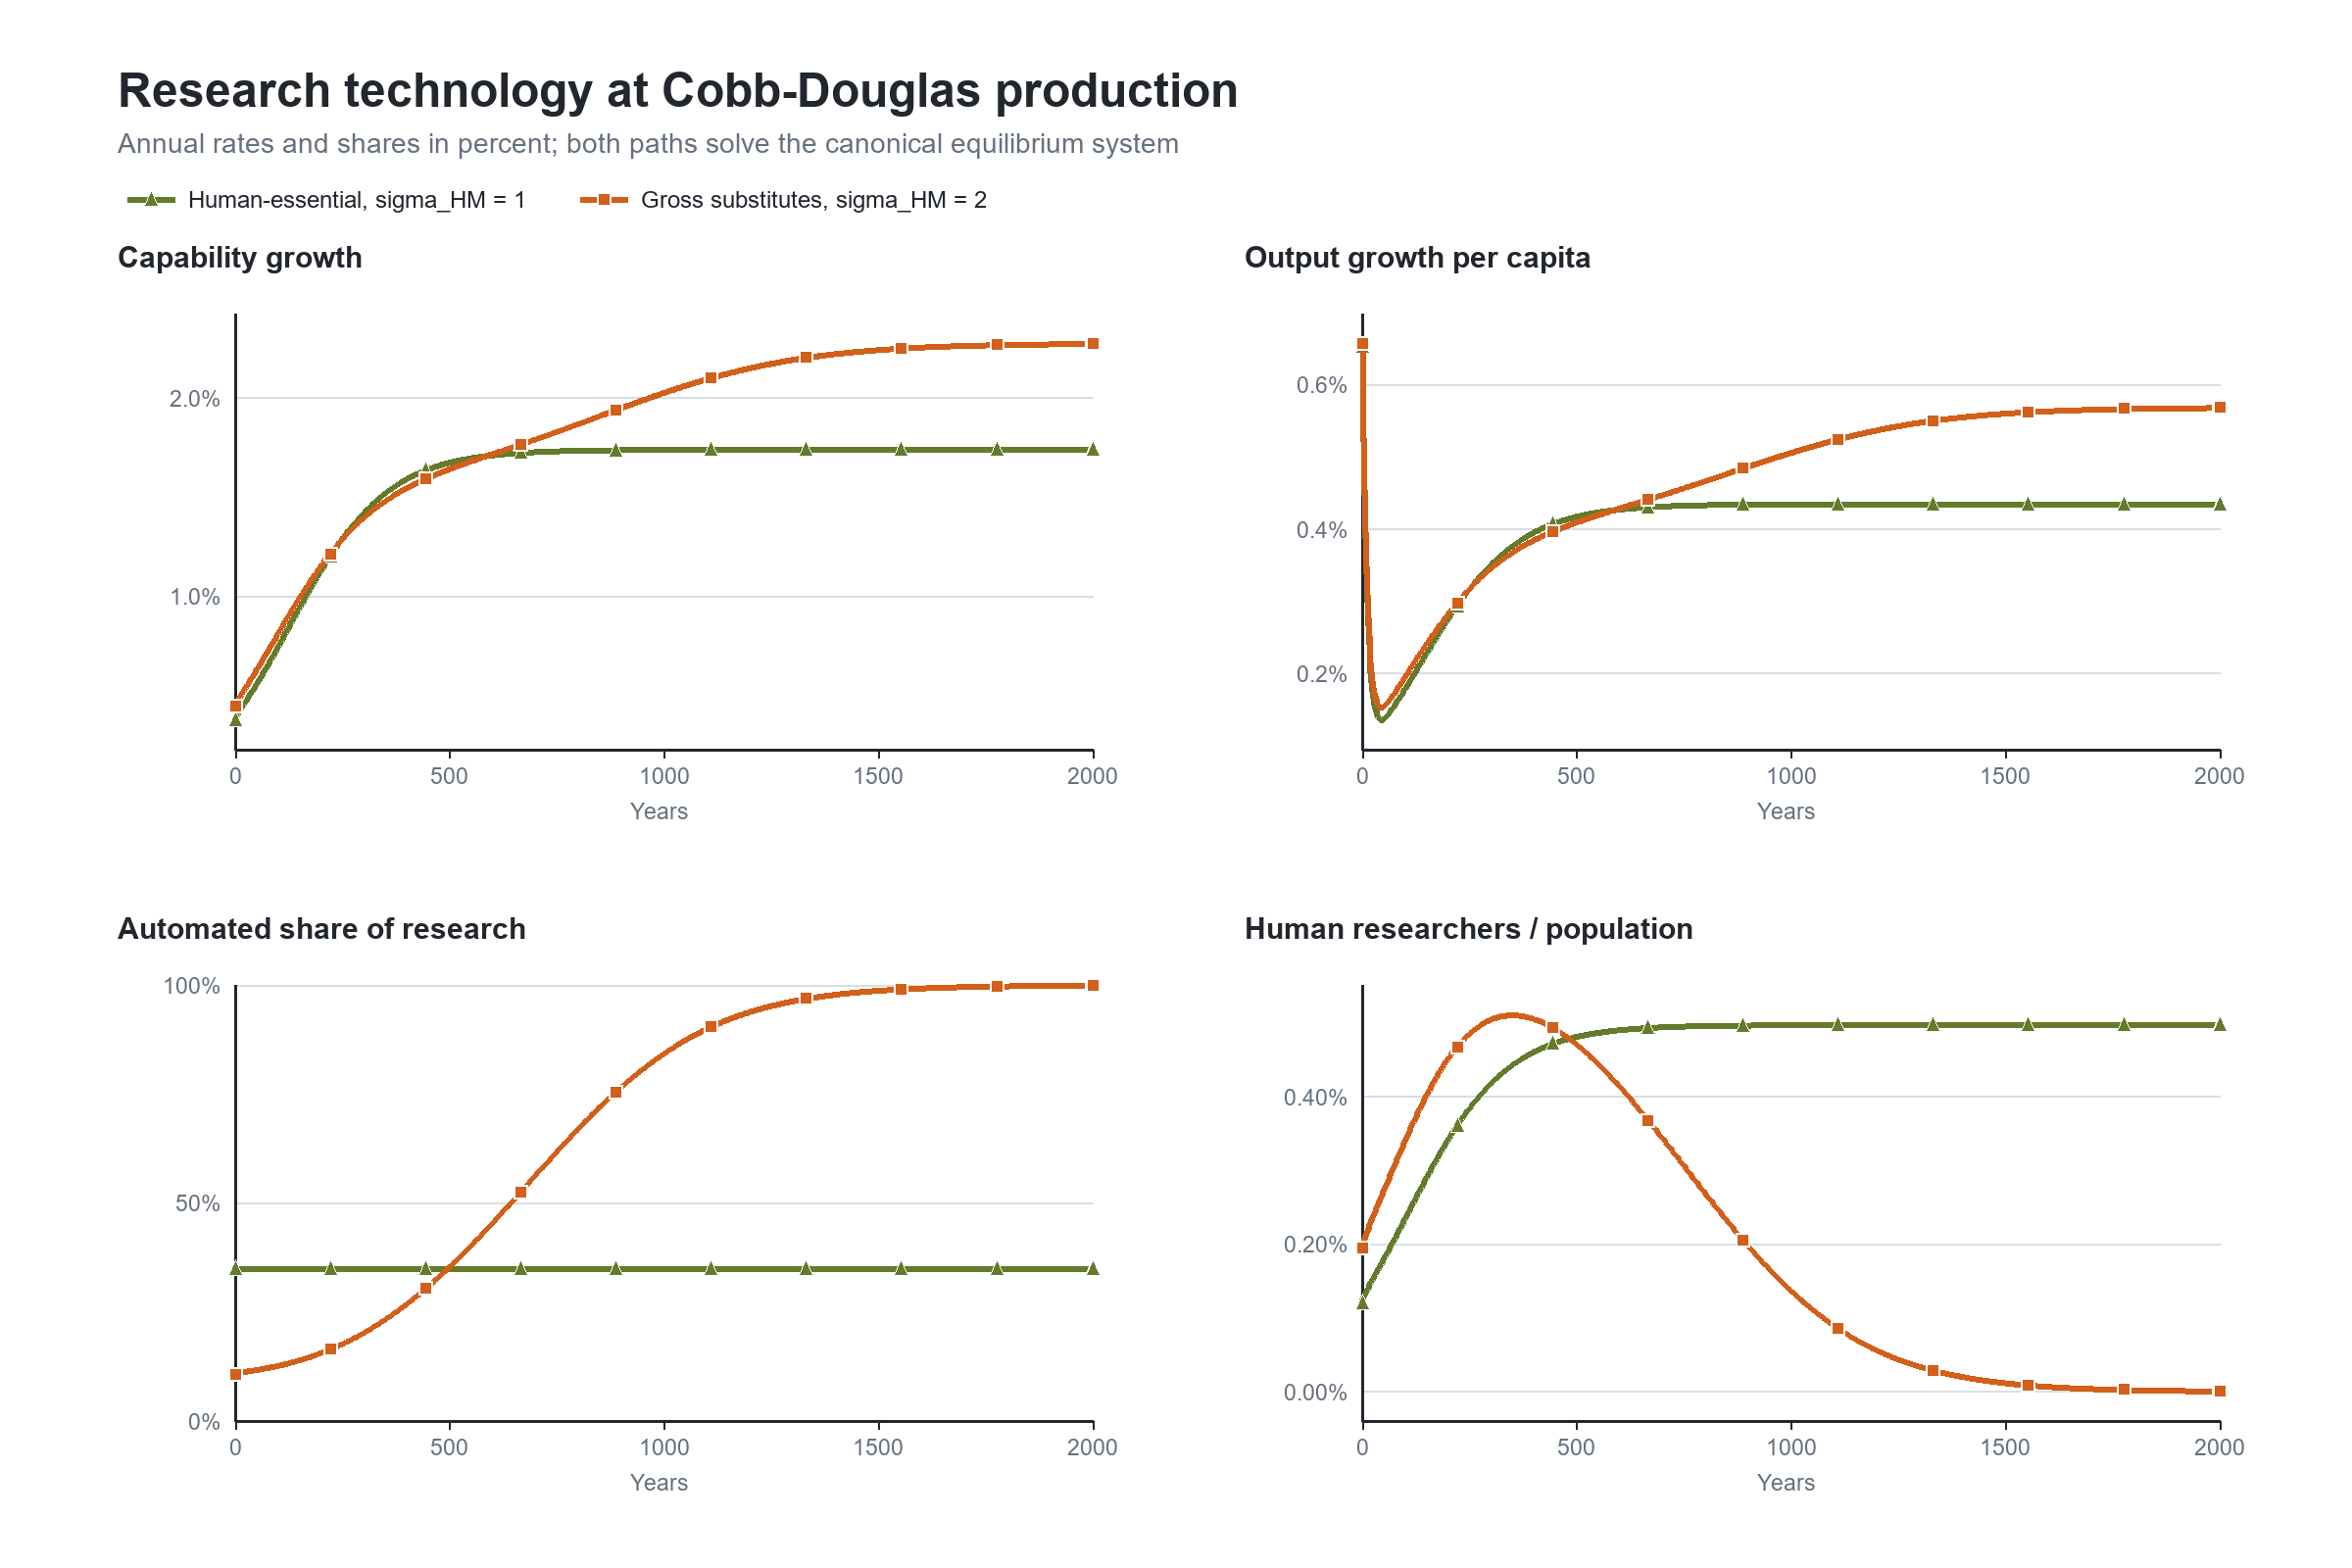
\includegraphics[width=\textwidth]{figures/equilibrium_research_technology_comparison.png}
    \caption{Research technology at Cobb--Douglas production. Both 2,000-year
    paths solve the canonical equilibrium system and share all parameters and
    initial stocks except $\sigma_{HM}$.}
    \label{fig:equilibrium-research-technology-comparison}
\end{figure}

\subsection{Case III: substitutable research at unit production elasticity}
\label{sec:case-substitutable-research}

\subsubsection{Analytical characterization}

Now set $\sigma_{XL}=1$ and $\sigma_{HM}>1$. Conditional
result~\ref{cond:ai-dominated-cd-limit} characterizes any nondegenerate
constant-growth limit in which the automated contribution tends to one. Such a
limit requires $D_{\mathrm{AI}}>0$. Capability growth and output-per-capita growth
are then $\eta n/D_{\mathrm{AI}}$ and
$(\omega_X/\omega_L)\eta n/D_{\mathrm{AI}}$, respectively. Unlike Case II, the
research contribution $s^M_t$ is endogenous and the feedback denominator moves
from its human-dominated value toward $D_{\mathrm{AI}}$. These statements are
conditional on the stated limit; the equilibrium computation determines whether
the transition actually approaches it from the chosen initial stocks.

\subsubsection{Equilibrium transition}

Along the equilibrium path, capability growth rises from 0.445 percent to 1.716
percent during the first 600 years and reaches 2.271 percent by year 2,000. Output-
and consumption-per-capita growth approach the analytical value of 0.568 percent,
and the net return converges to 4.568 percent. In
Figure~\ref{fig:equilibrium-research-technology-comparison}, the automated
contribution rises toward one and human research employment converges to zero.
Capability growth converges to 2.274 percent rather than the human-essential limit
of 1.738 percent. Gross substitution in research therefore changes both who
performs research and the strength of the feedback from output to capability.

\subsection{Cross-case comparisons: production, labor, and monopoly}

The next figures compare Cases I and III over a common 600-year window. They are
reported separately because the production chain, factor shares, resource
allocation, and monopoly outcomes are meaningful precisely as comparisons across
production regimes. Case II was isolated above to compare research technologies,
and Case IV is analyzed below on its endogenous free-boundary horizon.

Figure~\ref{fig:equilibrium-production-chain} follows the production tree rather
than placing all growing quantities in one panel. Under complementarity,
inference compute per capita falls even though capability rises. AI services per
capita still increase because each unit of compute becomes more productive, but
the service composite approaches a finite level. Under Cobb--Douglas production,
inference compute, AI services, and the service composite eventually become
log-linear. In both cases the real price of AI services falls, but much faster in
the Cobb--Douglas path.

\begin{figure}[H]
    \centering
    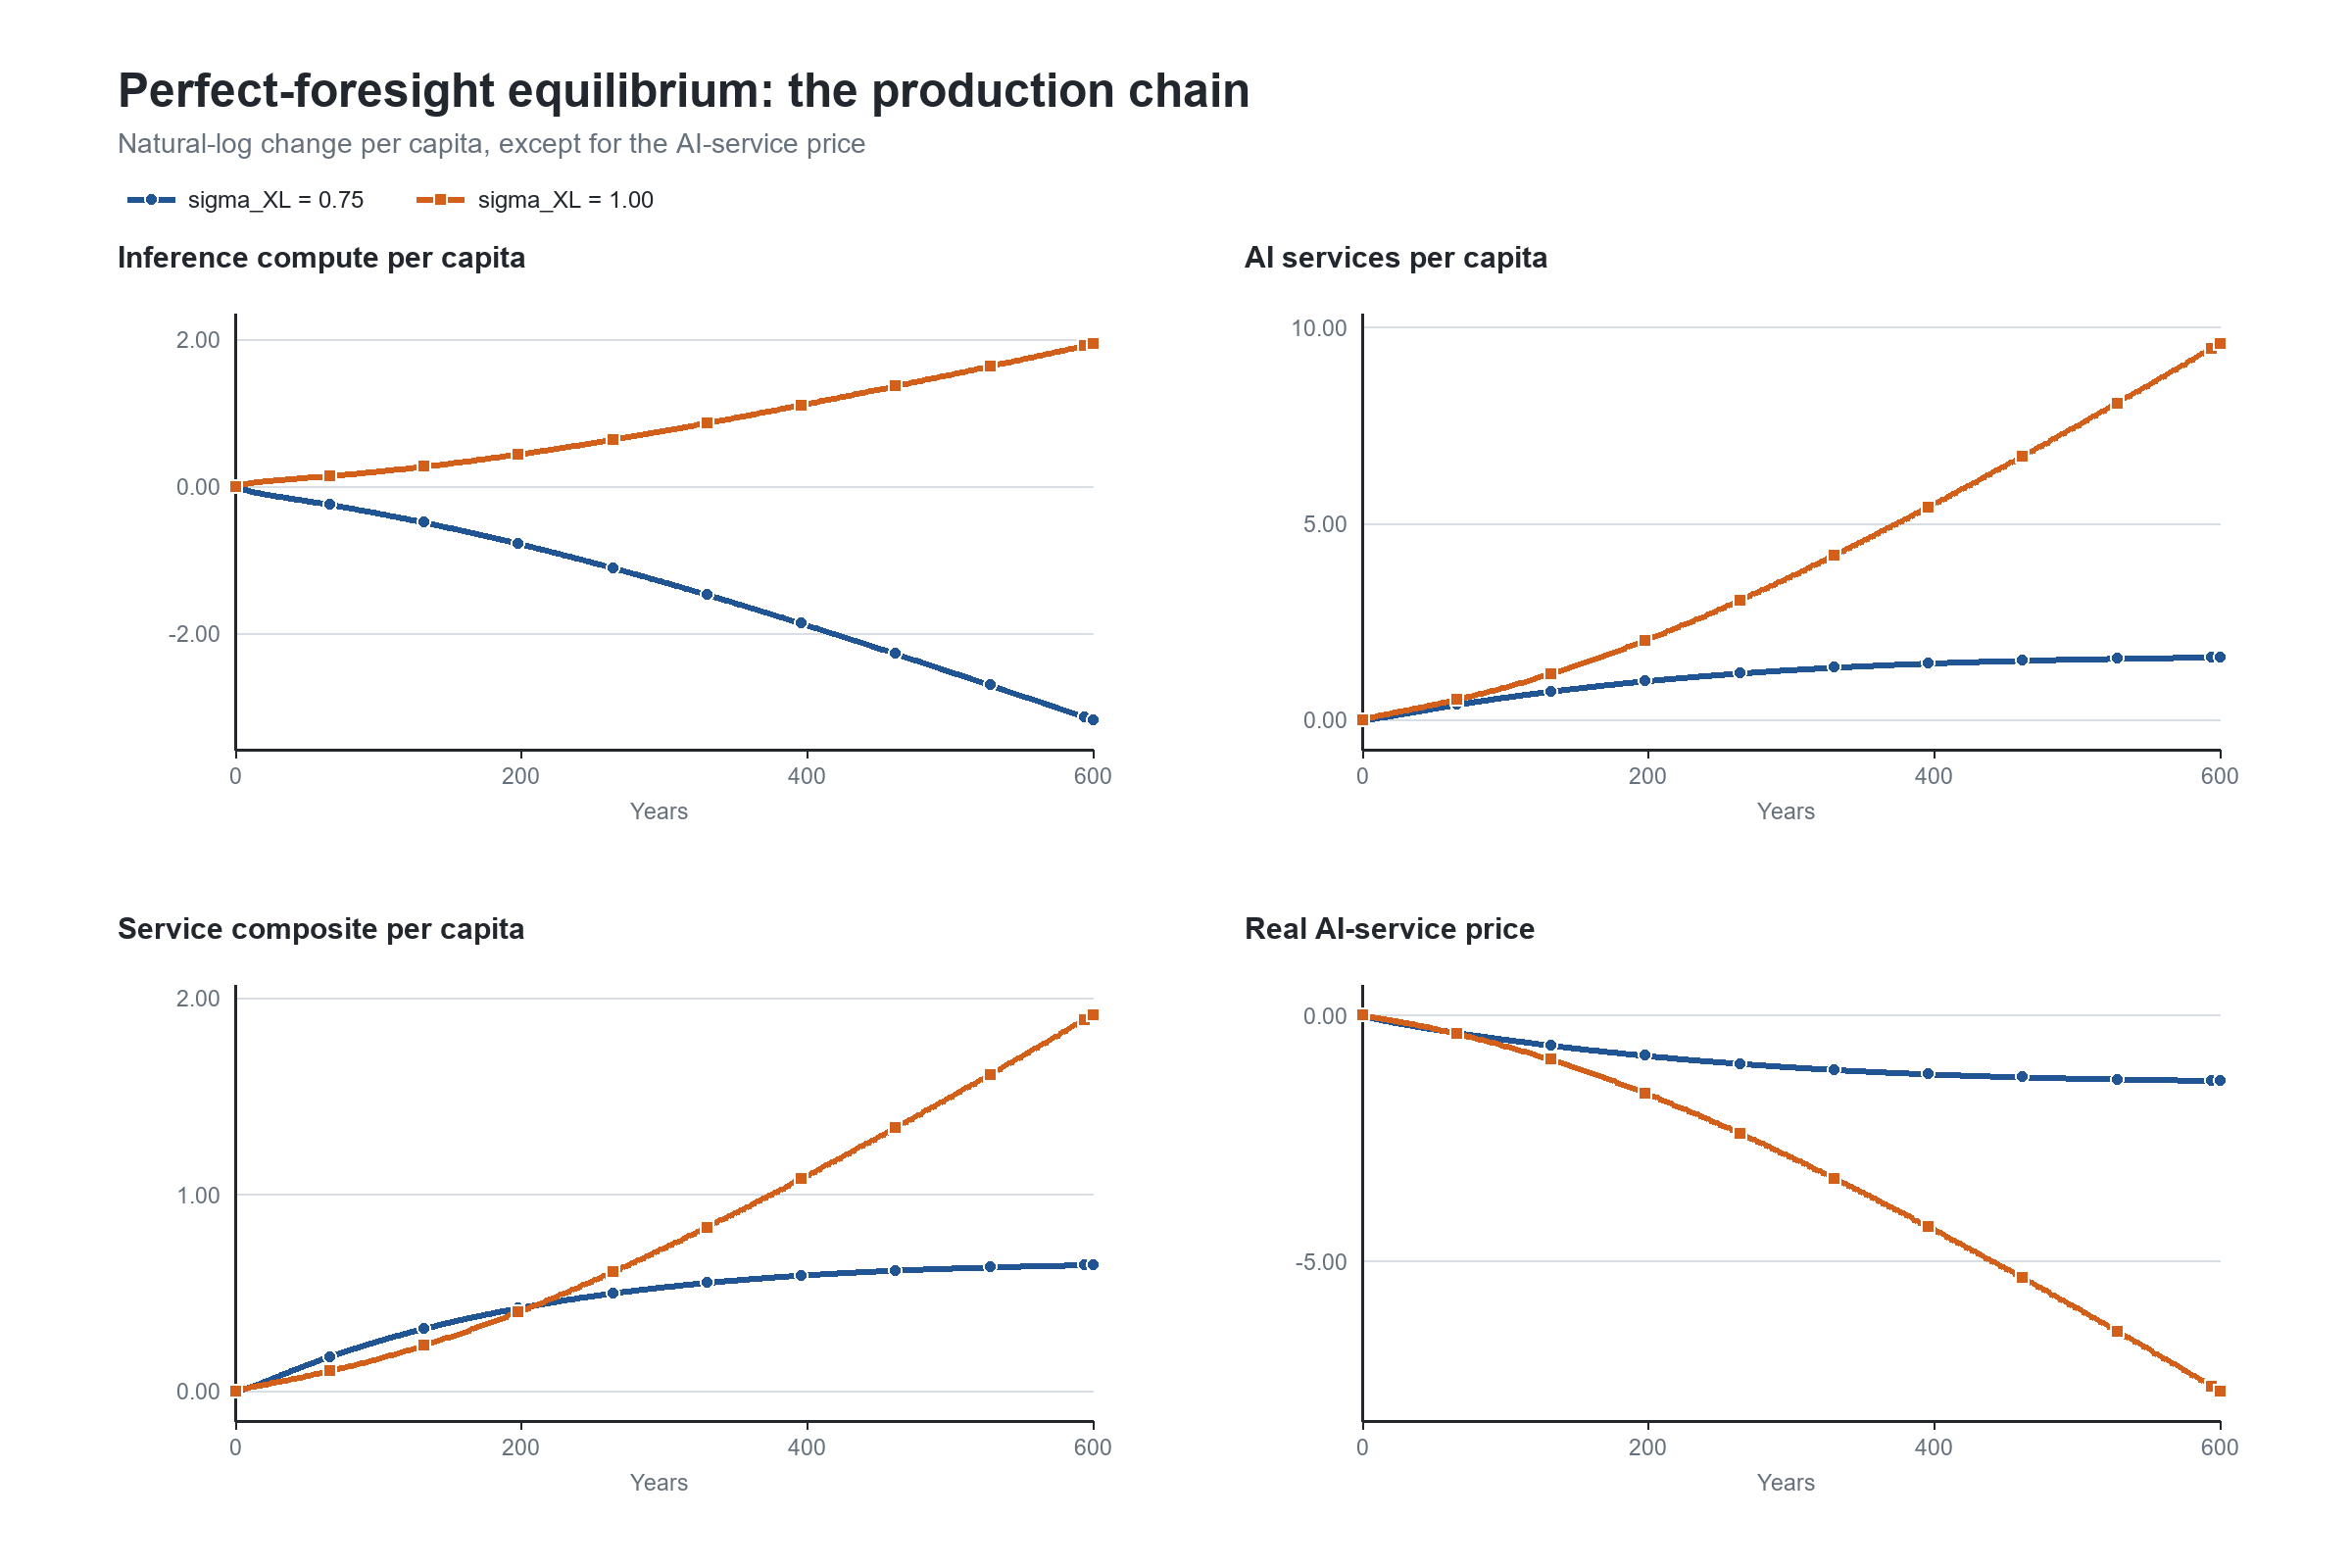
\includegraphics[width=\textwidth]{figures/equilibrium_production_chain.png}
    \caption{The equilibrium production chain. Quantity panels report
    natural-log changes per capita; the last panel reports the natural-log change
    in the real price of AI services.}
    \label{fig:equilibrium-production-chain}
\end{figure}

Figure~\ref{fig:equilibrium-factor-shares} reports the allocation of labor and
research. With $\sigma_{XL}=0.75$, the production-labor share rises from 36.05 to
44.46 percent as labor becomes the production bottleneck. The aggregate labor share
rises by almost the same amount because human research employment falls from 1.38
percent to 0.016 percent of the population. The automated contribution to research
increases only from 6.02 to 12.23 percent. A research elasticity above one does not
make automation dominant when the wage remains bounded.

Under Cobb--Douglas production, the production-labor share remains fixed at 53.60
percent. The automated research share rises from 10.60 percent to 45.35 percent by
year 600 and to 99.93 percent by year 2,000. Human research employment is
non-monotone: it rises from 0.19 percent of the population to approximately 0.5
percent and then tends to zero. The development industry can therefore expand its
use of human researchers during part of the automation transition even though
human input eventually becomes negligible relative to automated research.

\begin{figure}[H]
    \centering
    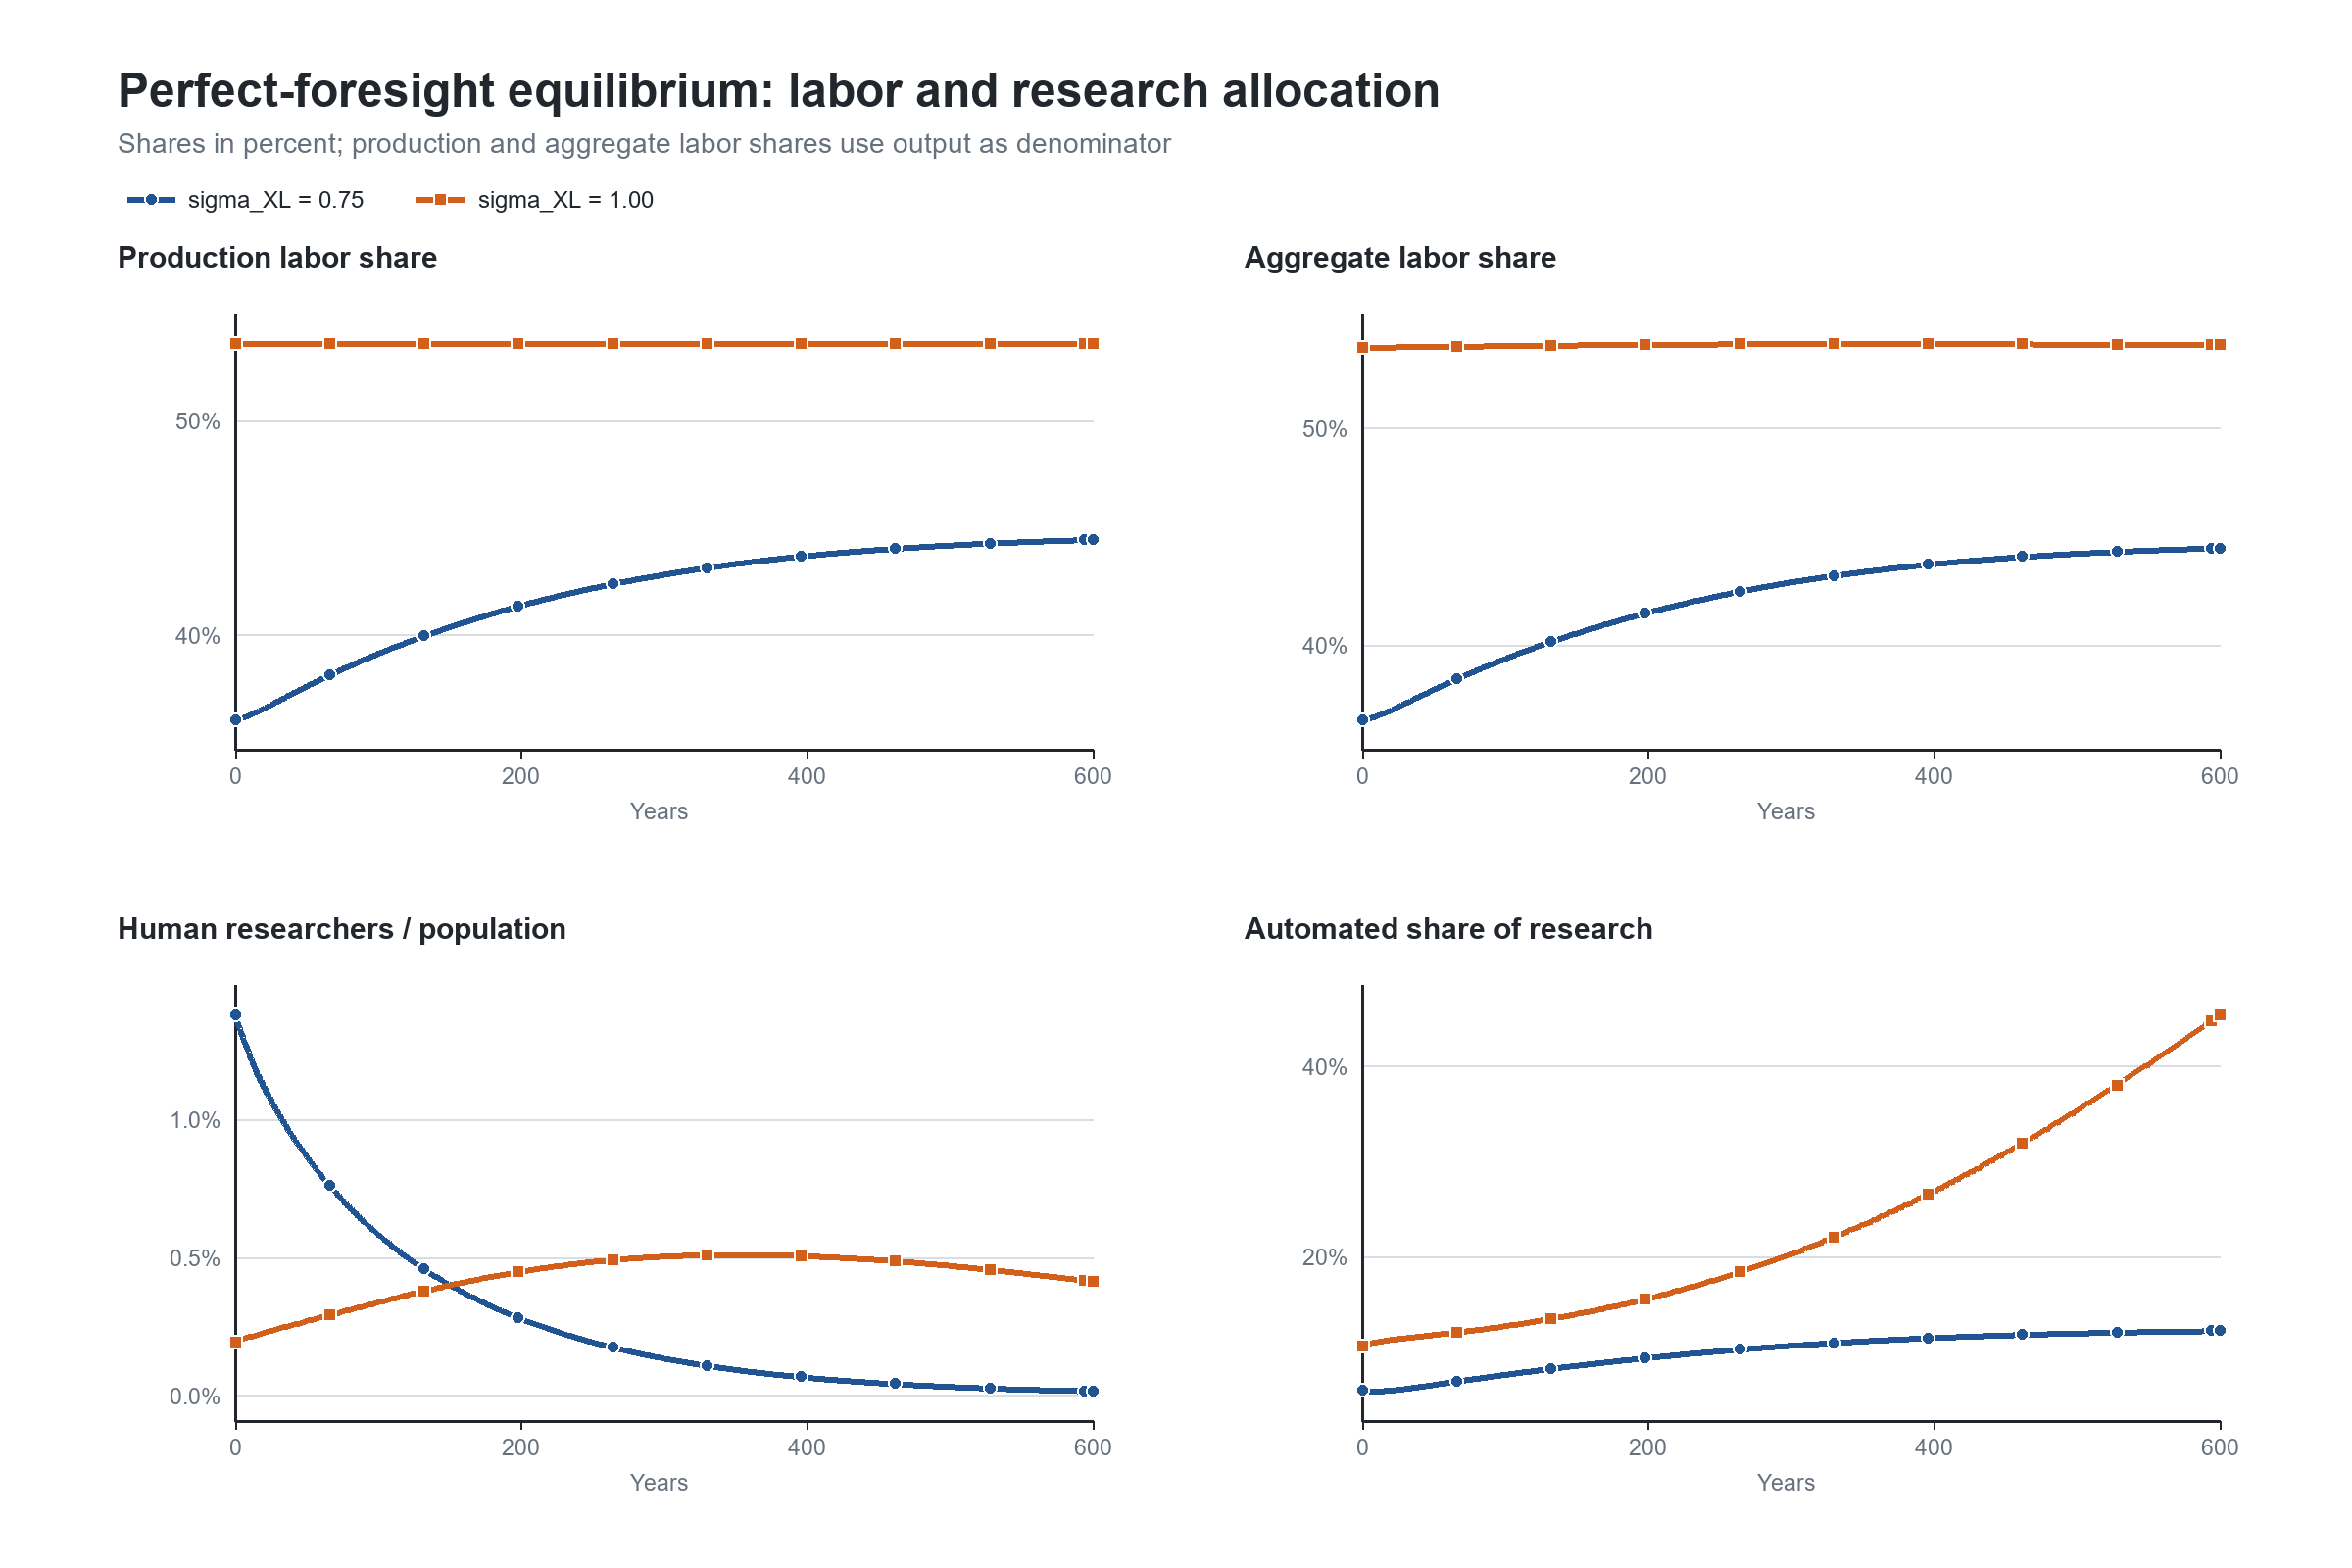
\includegraphics[width=\textwidth]{figures/equilibrium_factor_shares.png}
    \caption{Labor-income shares and the equilibrium research allocation. The
    aggregate labor share includes both production workers and human researchers.}
    \label{fig:equilibrium-factor-shares}
\end{figure}

Figure~\ref{fig:equilibrium-research-chain} makes the distinction between scale
and composition explicit. Under complementarity, human, automated, and effective
research all contract per capita, even though the automated contribution to the
research CES rises. Under Cobb--Douglas production, human research per capita is
temporarily hump-shaped while automated and effective research expand. The
human-to-machine ratio falls in both paths, but the aggregate scale consequences
are opposite. A falling $H/M$ is therefore not, by itself, evidence that the AI
development sector is expanding.

\begin{figure}[H]
    \centering
    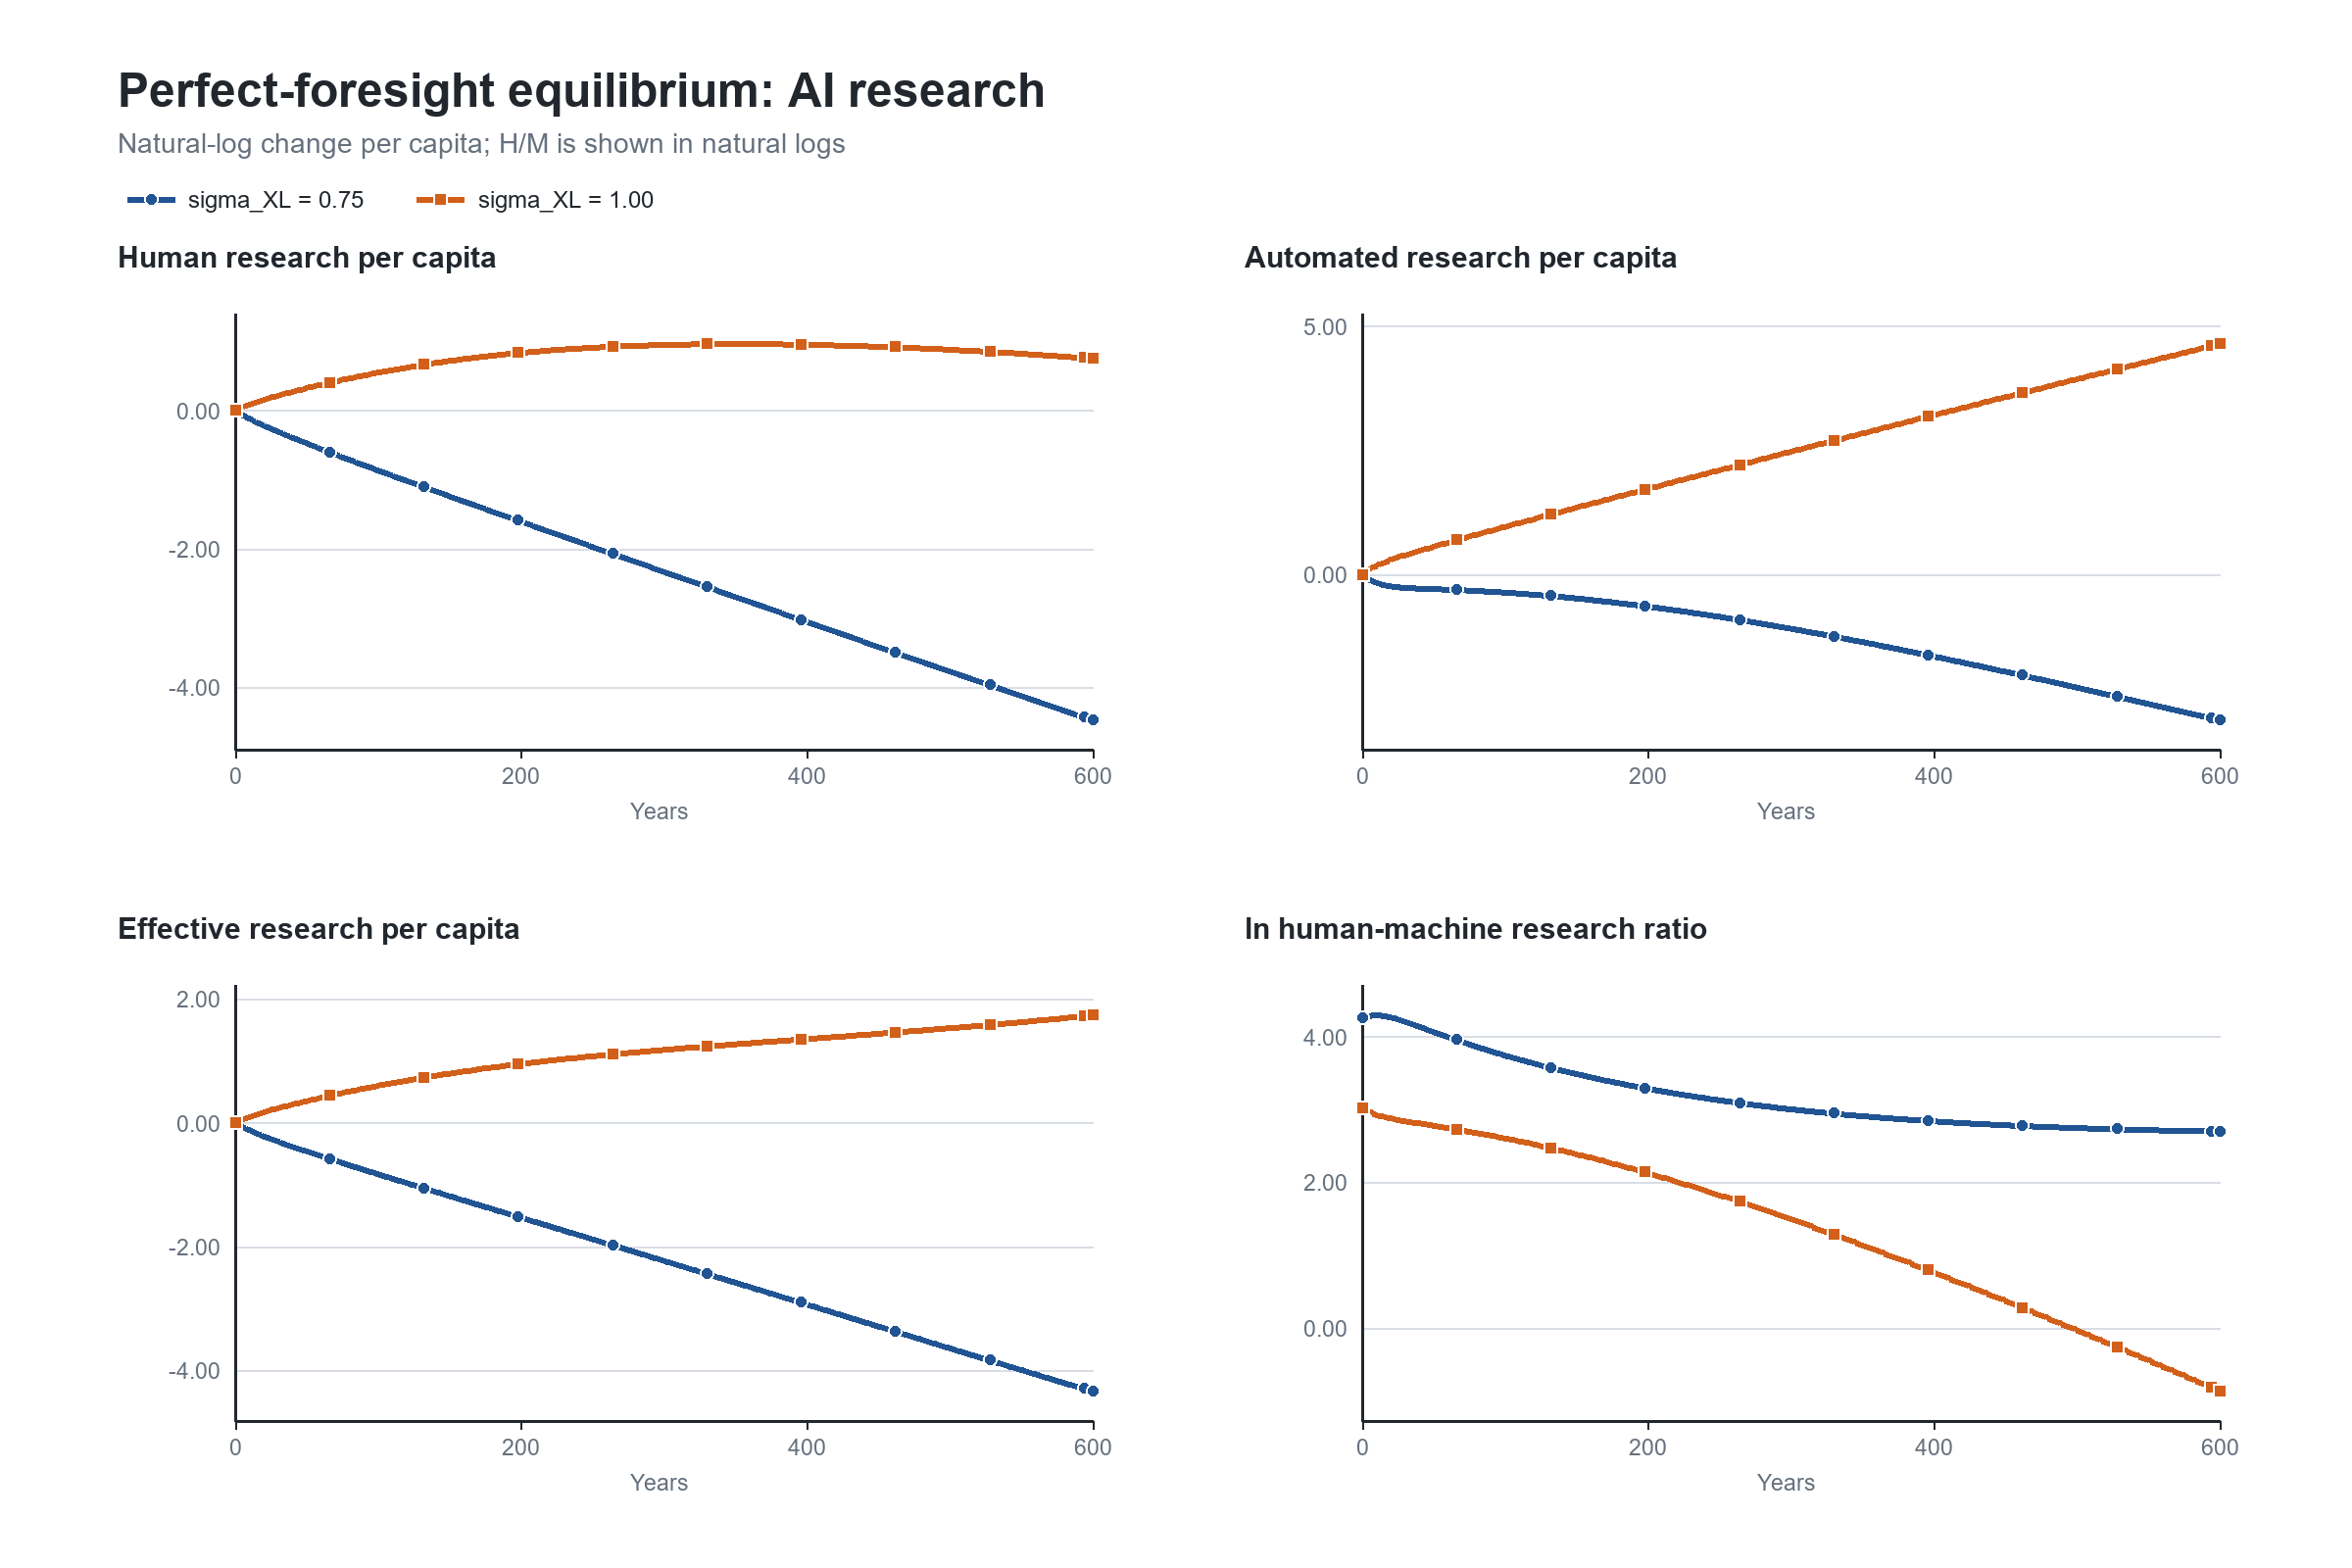
\includegraphics[width=\textwidth]{figures/equilibrium_research_chain.png}
    \caption{The equilibrium research chain. The first three panels report
    natural-log changes per capita; the final panel reports $\ln(H/M)$.}
    \label{fig:equilibrium-research-chain}
\end{figure}

The 600-year comparison understates how slowly the Cobb--Douglas limit emerges.
Figure~\ref{fig:equilibrium-cd-long-run} therefore reports the full 2,000-year
path separately. Capability and output growth approach constants only after the
automated contribution to research has moved close to one and human research has
become negligible relative to population. This separate long-horizon panel avoids
compressing the economically relevant first centuries of the complementarity
experiment.

\begin{figure}[H]
    \centering
    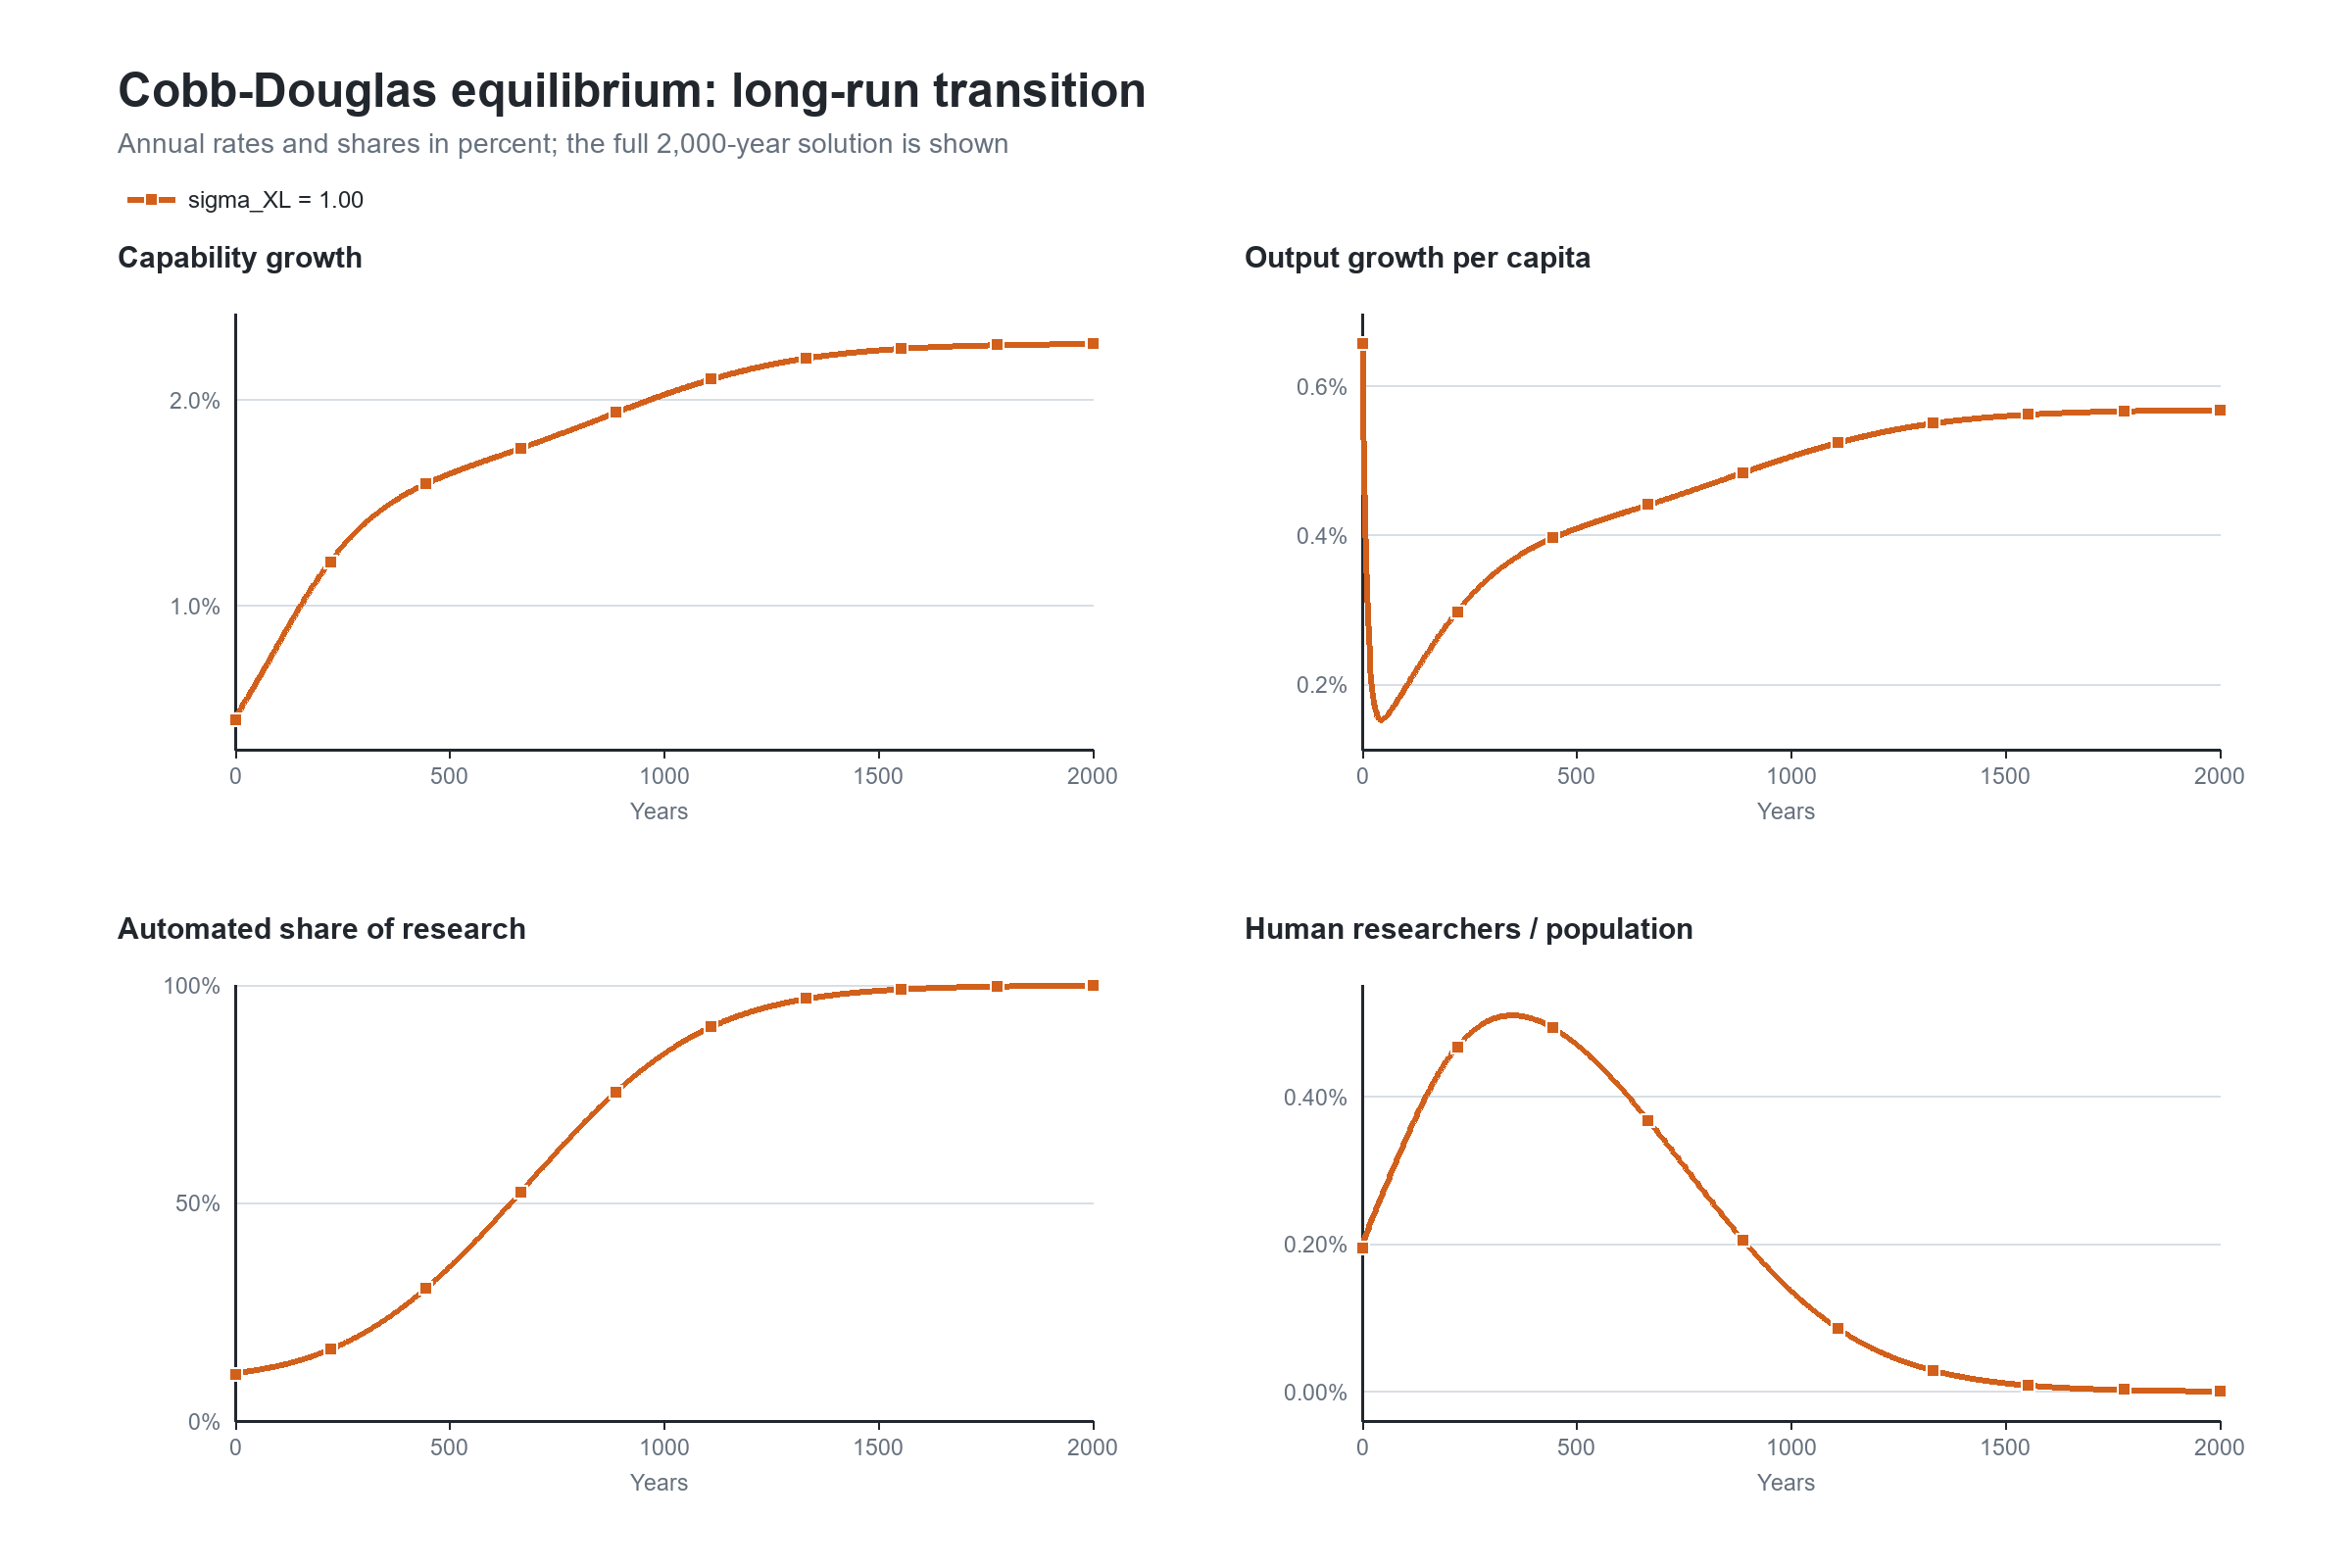
\includegraphics[width=\textwidth]{figures/equilibrium_cobb_douglas_long_run.png}
    \caption{Long-run Cobb--Douglas transition. The figure shows the complete
    2,000-year equilibrium solution rather than truncating it to the common
    600-year comparison window.}
    \label{fig:equilibrium-cd-long-run}
\end{figure}

Figures~\ref{fig:equilibrium-resource-allocation} and
\ref{fig:equilibrium-monopoly-block} close the accounting and monopoly blocks.
The four resource shares add to one at every date. Under complementarity,
inference and automated-research spending become negligible relative to output;
under Cobb--Douglas production, inference spending remains constant as a share of
output while automated-research spending gradually rises. Market power also has
different manifestations. With Cobb--Douglas demand the markup and operating
profit share are constant. Under complementarity, the price falls much more slowly
than marginal cost, so the markup rises sharply even as operating profits decline
as a share of output. The markup alone is therefore not a sufficient measure of
the developer's aggregate rents.

\begin{figure}[H]
    \centering
    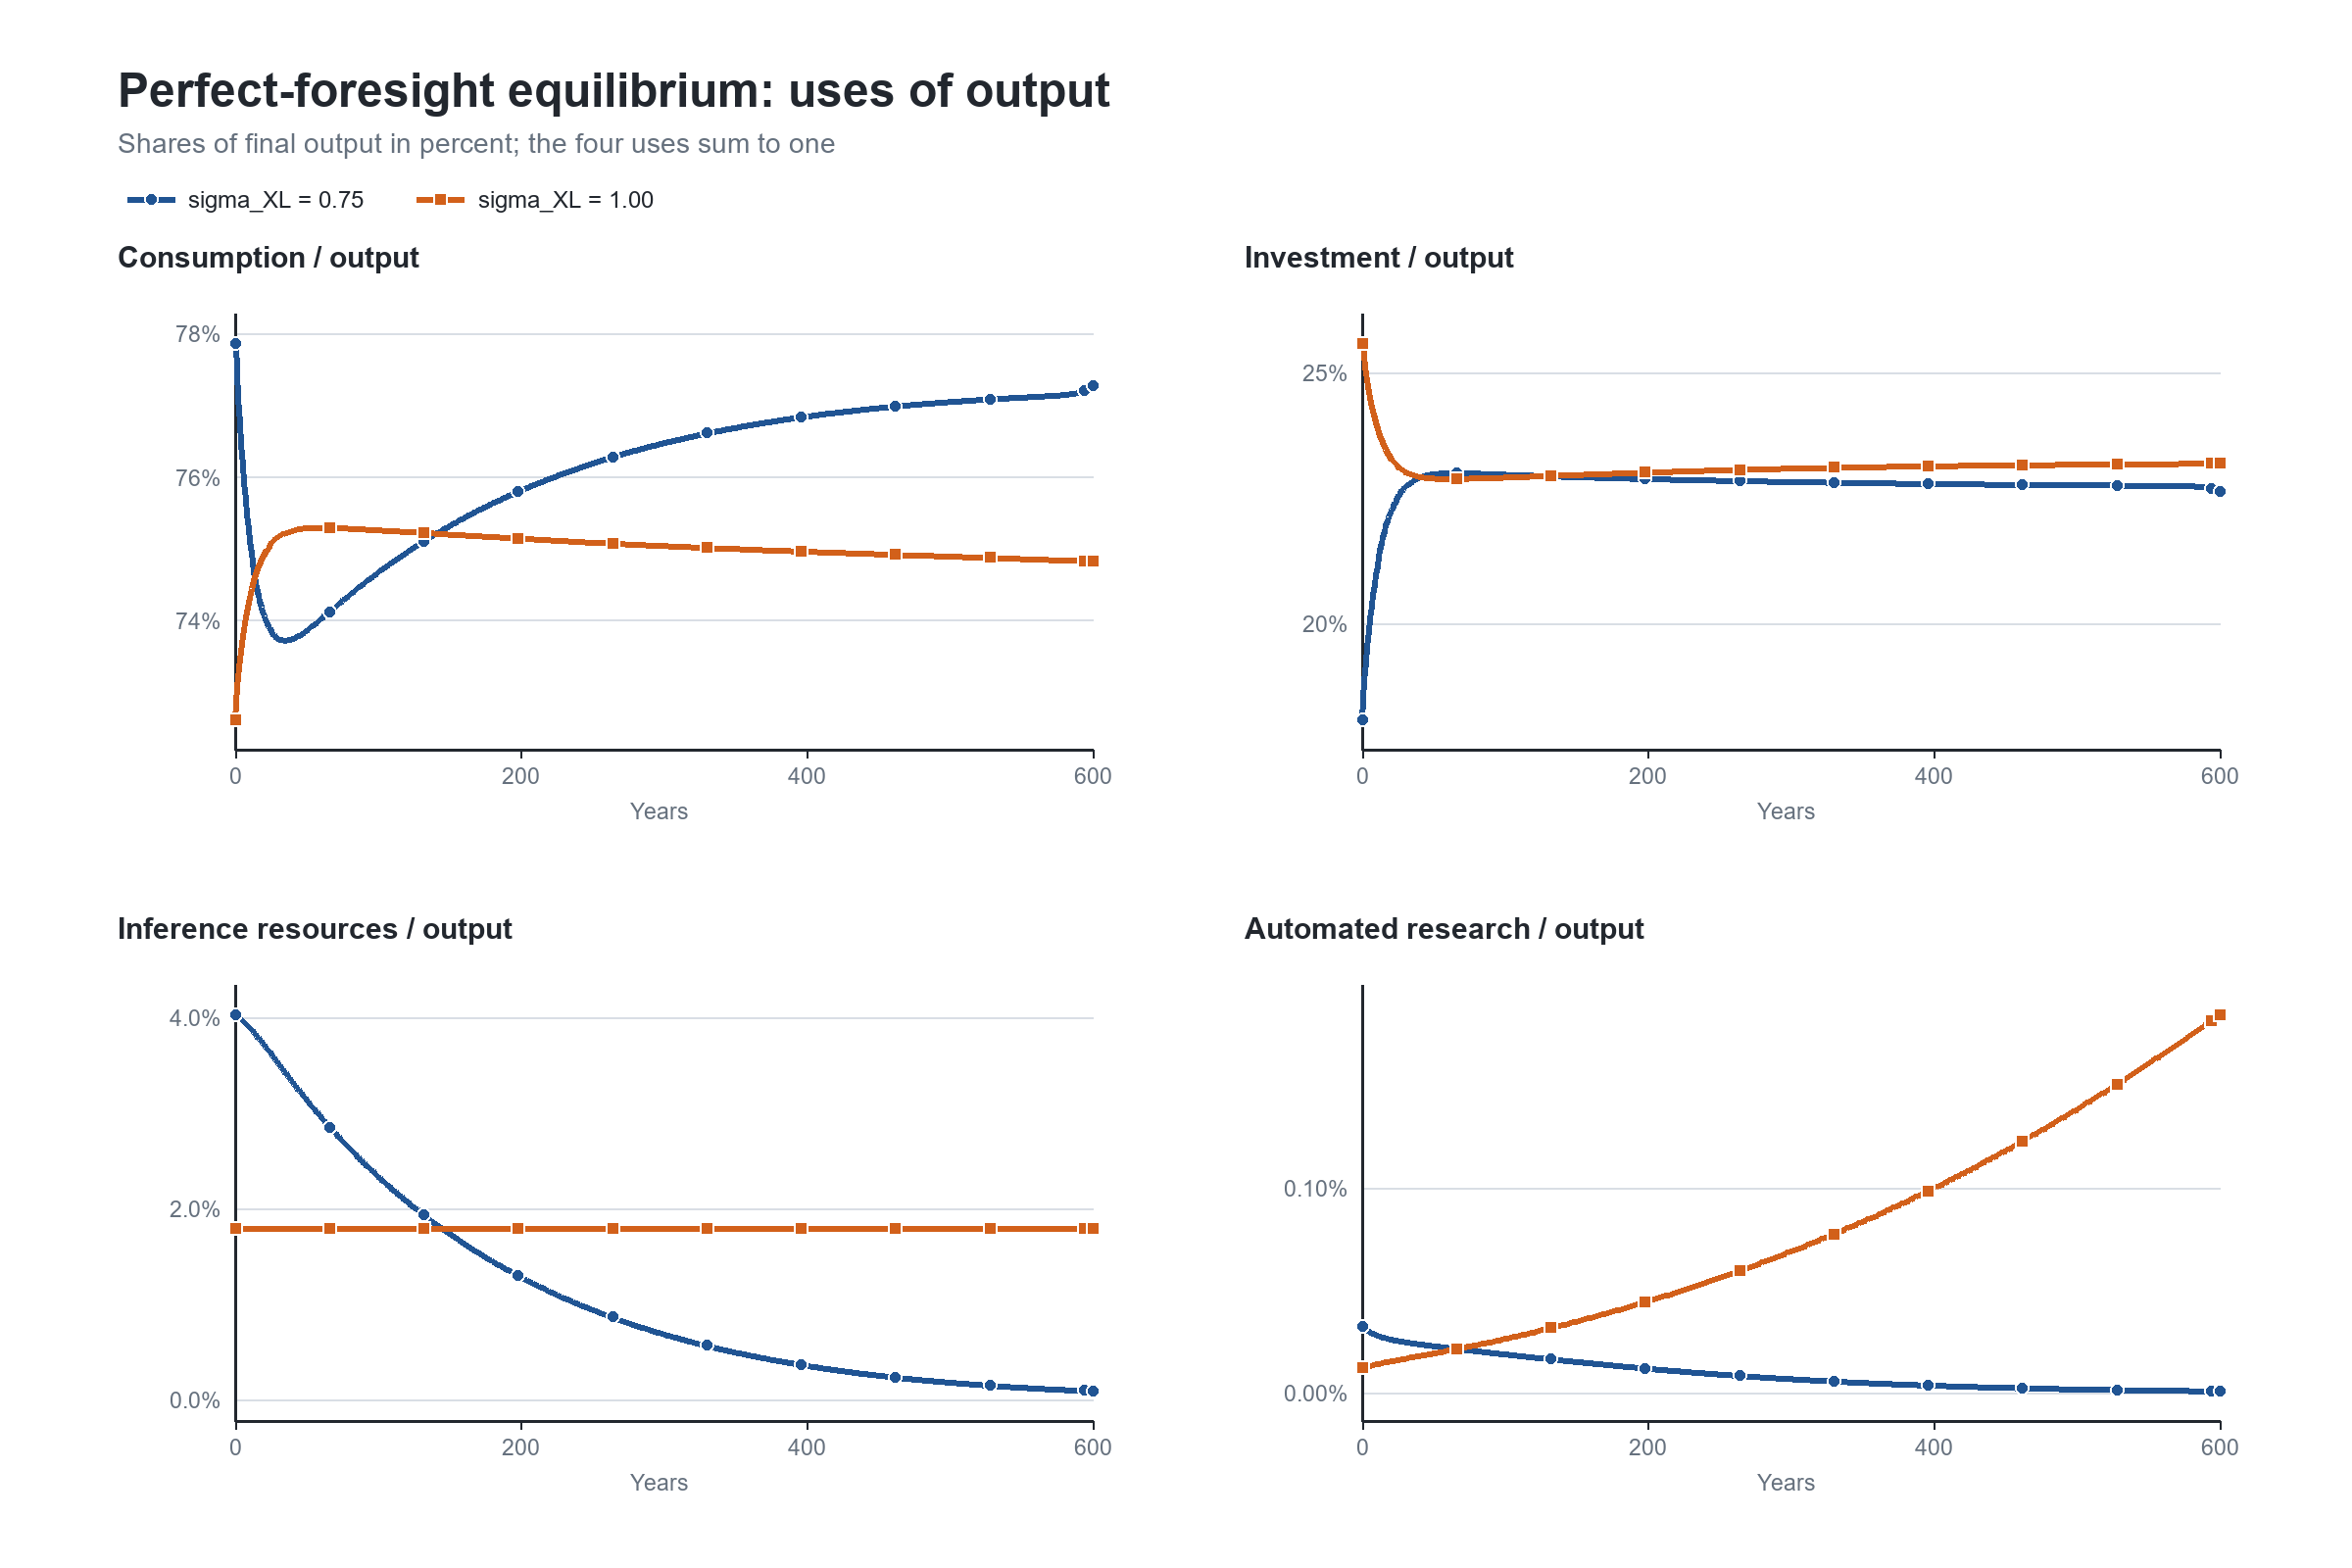
\includegraphics[width=\textwidth]{figures/equilibrium_resource_allocation.png}
    \caption{Equilibrium allocation of final output. The panels show $C/Y$,
    $I/Y$, $\xi U/Y$, and $\xi M/Y$ in percent.}
    \label{fig:equilibrium-resource-allocation}
\end{figure}

\begin{figure}[H]
    \centering
    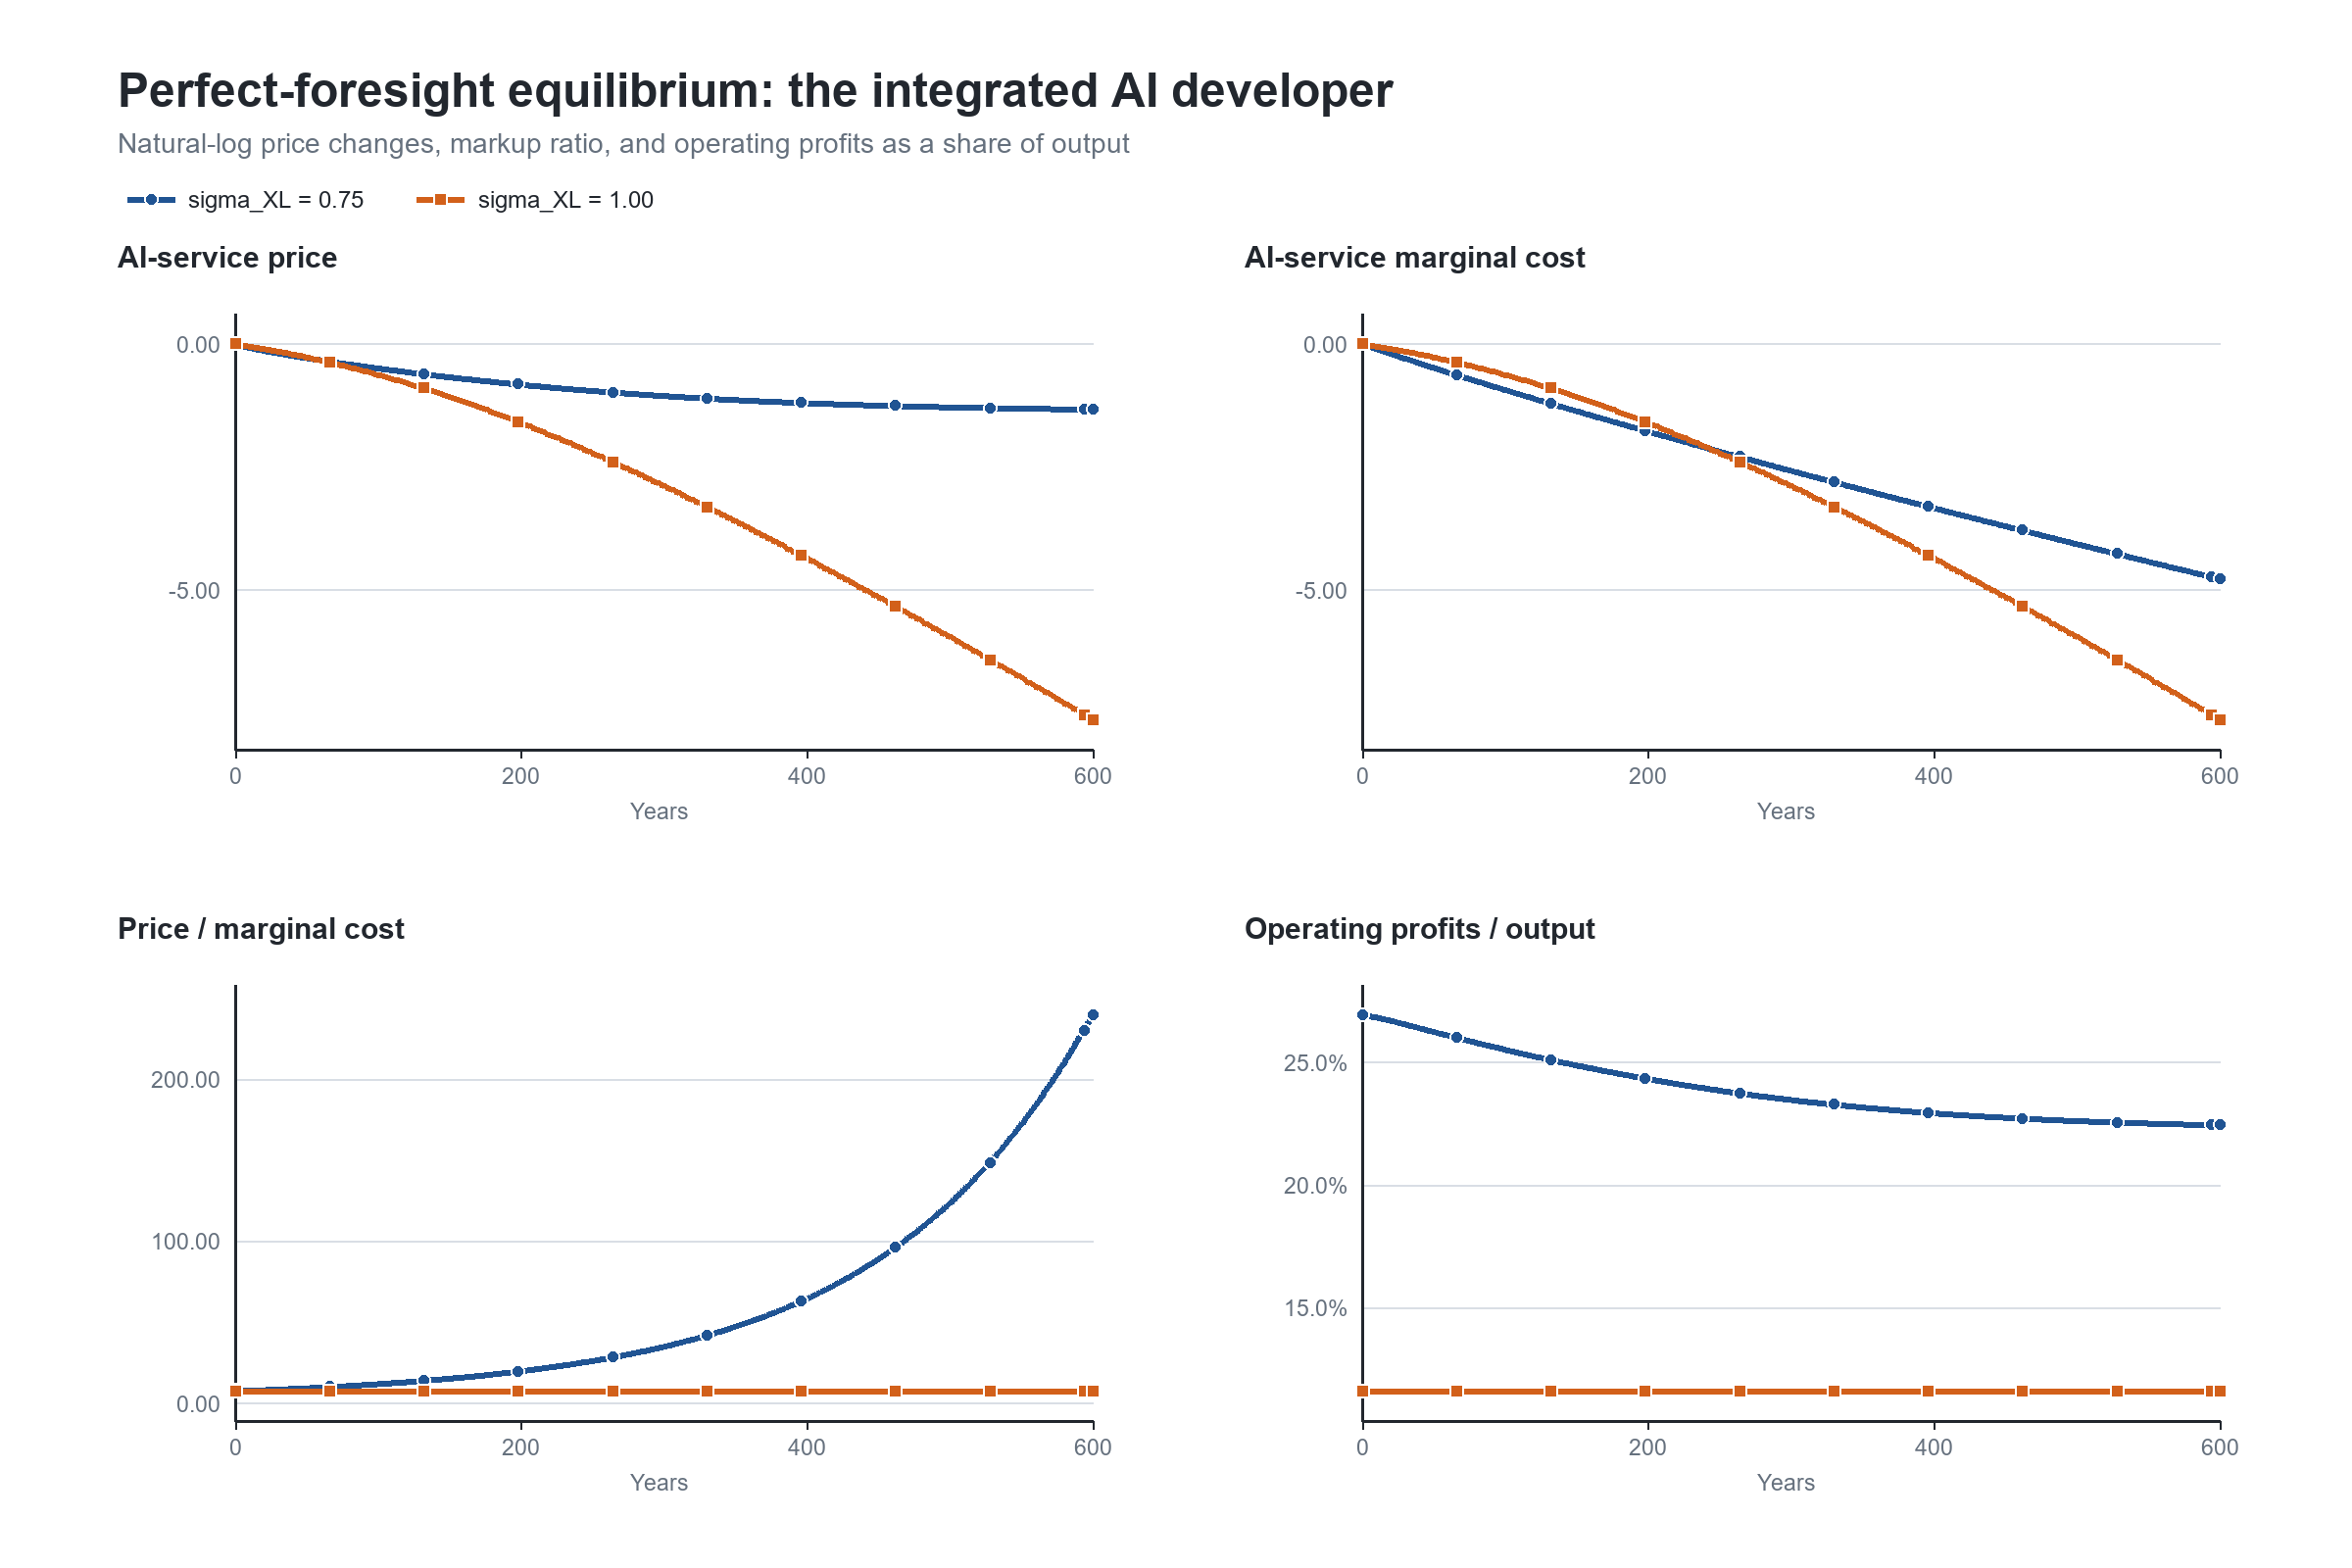
\includegraphics[width=\textwidth]{figures/equilibrium_monopoly_block.png}
    \caption{The integrated AI developer. Price and marginal cost are natural-log
    changes; the markup is the price--marginal-cost ratio and operating profits
    are reported as a share of output.}
    \label{fig:equilibrium-monopoly-block}
\end{figure}

\subsection{Case IV: production gross substitution, $\sigma_{XL}>1$}
\label{sec:case-production-substitutes}

\subsubsection{Analytical characterization}

Proposition~\ref{prop:gross-substitution-no-steady-state} rules out an interior
finite-rate steady state with positive capability growth. As capability lowers the
resource cost of AI services, an exact equilibrium lower bound makes $Y/K$ rise
without bound even without assuming a path for the endogenous AI expenditure
share. The return to capital and the growth rate implied by the Euler equation
therefore cannot converge to finite constants. If the normalized AI-service cost
also vanishes, the stronger result $s^X_t\to1$ follows. Conditional
result~\ref{cond:high-sigma-singular-scaling} goes further under its stated
AI-dominated scaling and characterizes a finite-time singular branch. The
nonexistence proposition does not by itself prove that the optimizing equilibrium
selects that branch; it may encounter an allocation boundary first.

\subsubsection{Free-boundary equilibrium transitions}

The core production-acceleration configuration uses $\sigma_{XL}=1.35$. The
$\sigma_{XL}=1.50$ and 2.00 paths check how substitution changes the timing of the
same regime. All three values lie below the static wage threshold $1/\alpha$. This restriction
makes the direct effect of an AI-service expansion on the wage positive, but does
not by itself determine the equilibrium wage path. The simulations verify that the
wage rises and automated research becomes asymptotically dominant. Table
\ref{tab:high-sigma-equilibrium-summary} reports the terminal boundary, the
endogenous time at which the path reaches it, and
\begin{equation}
    \widehat T^*
    =
    T+\frac{1}{\vartheta\bar a\,z_T},
    \label{eq:estimated-singularity-time}
\end{equation}
which follows from equation~\eqref{eq:high-sigma-time-to-singularity}. The final
column reports the smallest wage-growth rate along each path, not its terminal
value.

\begin{table}[htbp]
    \centering
    \caption{Free-boundary equilibrium paths with $\sigma_{XL}>1$}
    \label{tab:high-sigma-equilibrium-summary}
    \begin{tabular}{cccccc}
        \toprule
        $\sigma_{XL}$ & $z_T$ & $T$ & $\widehat T^*$
        & first year $g_{Y/N}\geq5\%$ & $\min_t g_w$ \\
        \midrule
        1.35 & 50  & 333.22 & 333.38 & 297 & 0.070\% \\
        1.50 & 50  & 280.29 & 280.45 & 247 & 0.054\% \\
        2.00 & 100 & 209.00 & 209.08 & 180 & 0.028\% \\
        \bottomrule
    \end{tabular}
    \begin{minipage}{0.96\textwidth}
    \footnotesize\emph{Notes:} Calendar time is measured from the common initial
    stocks. The dates are conditional on the illustrative parameter values in
    Table~\ref{tab:equilibrium-numerical-parameters}; they are not calibrated
    forecasts.
    \end{minipage}
\end{table}

Figure~\ref{fig:high-sigma-equilibrium-levels} shows a long interval of moderate
growth followed by a sharp acceleration. Moving $\sigma_{XL}$ from 1.35 to 2.00
brings the acceleration forward by more than a century. The comparison is not
generated by different investment or research-spending rules: the household and
the developer optimize along every path.

\begin{figure}[H]
    \centering
    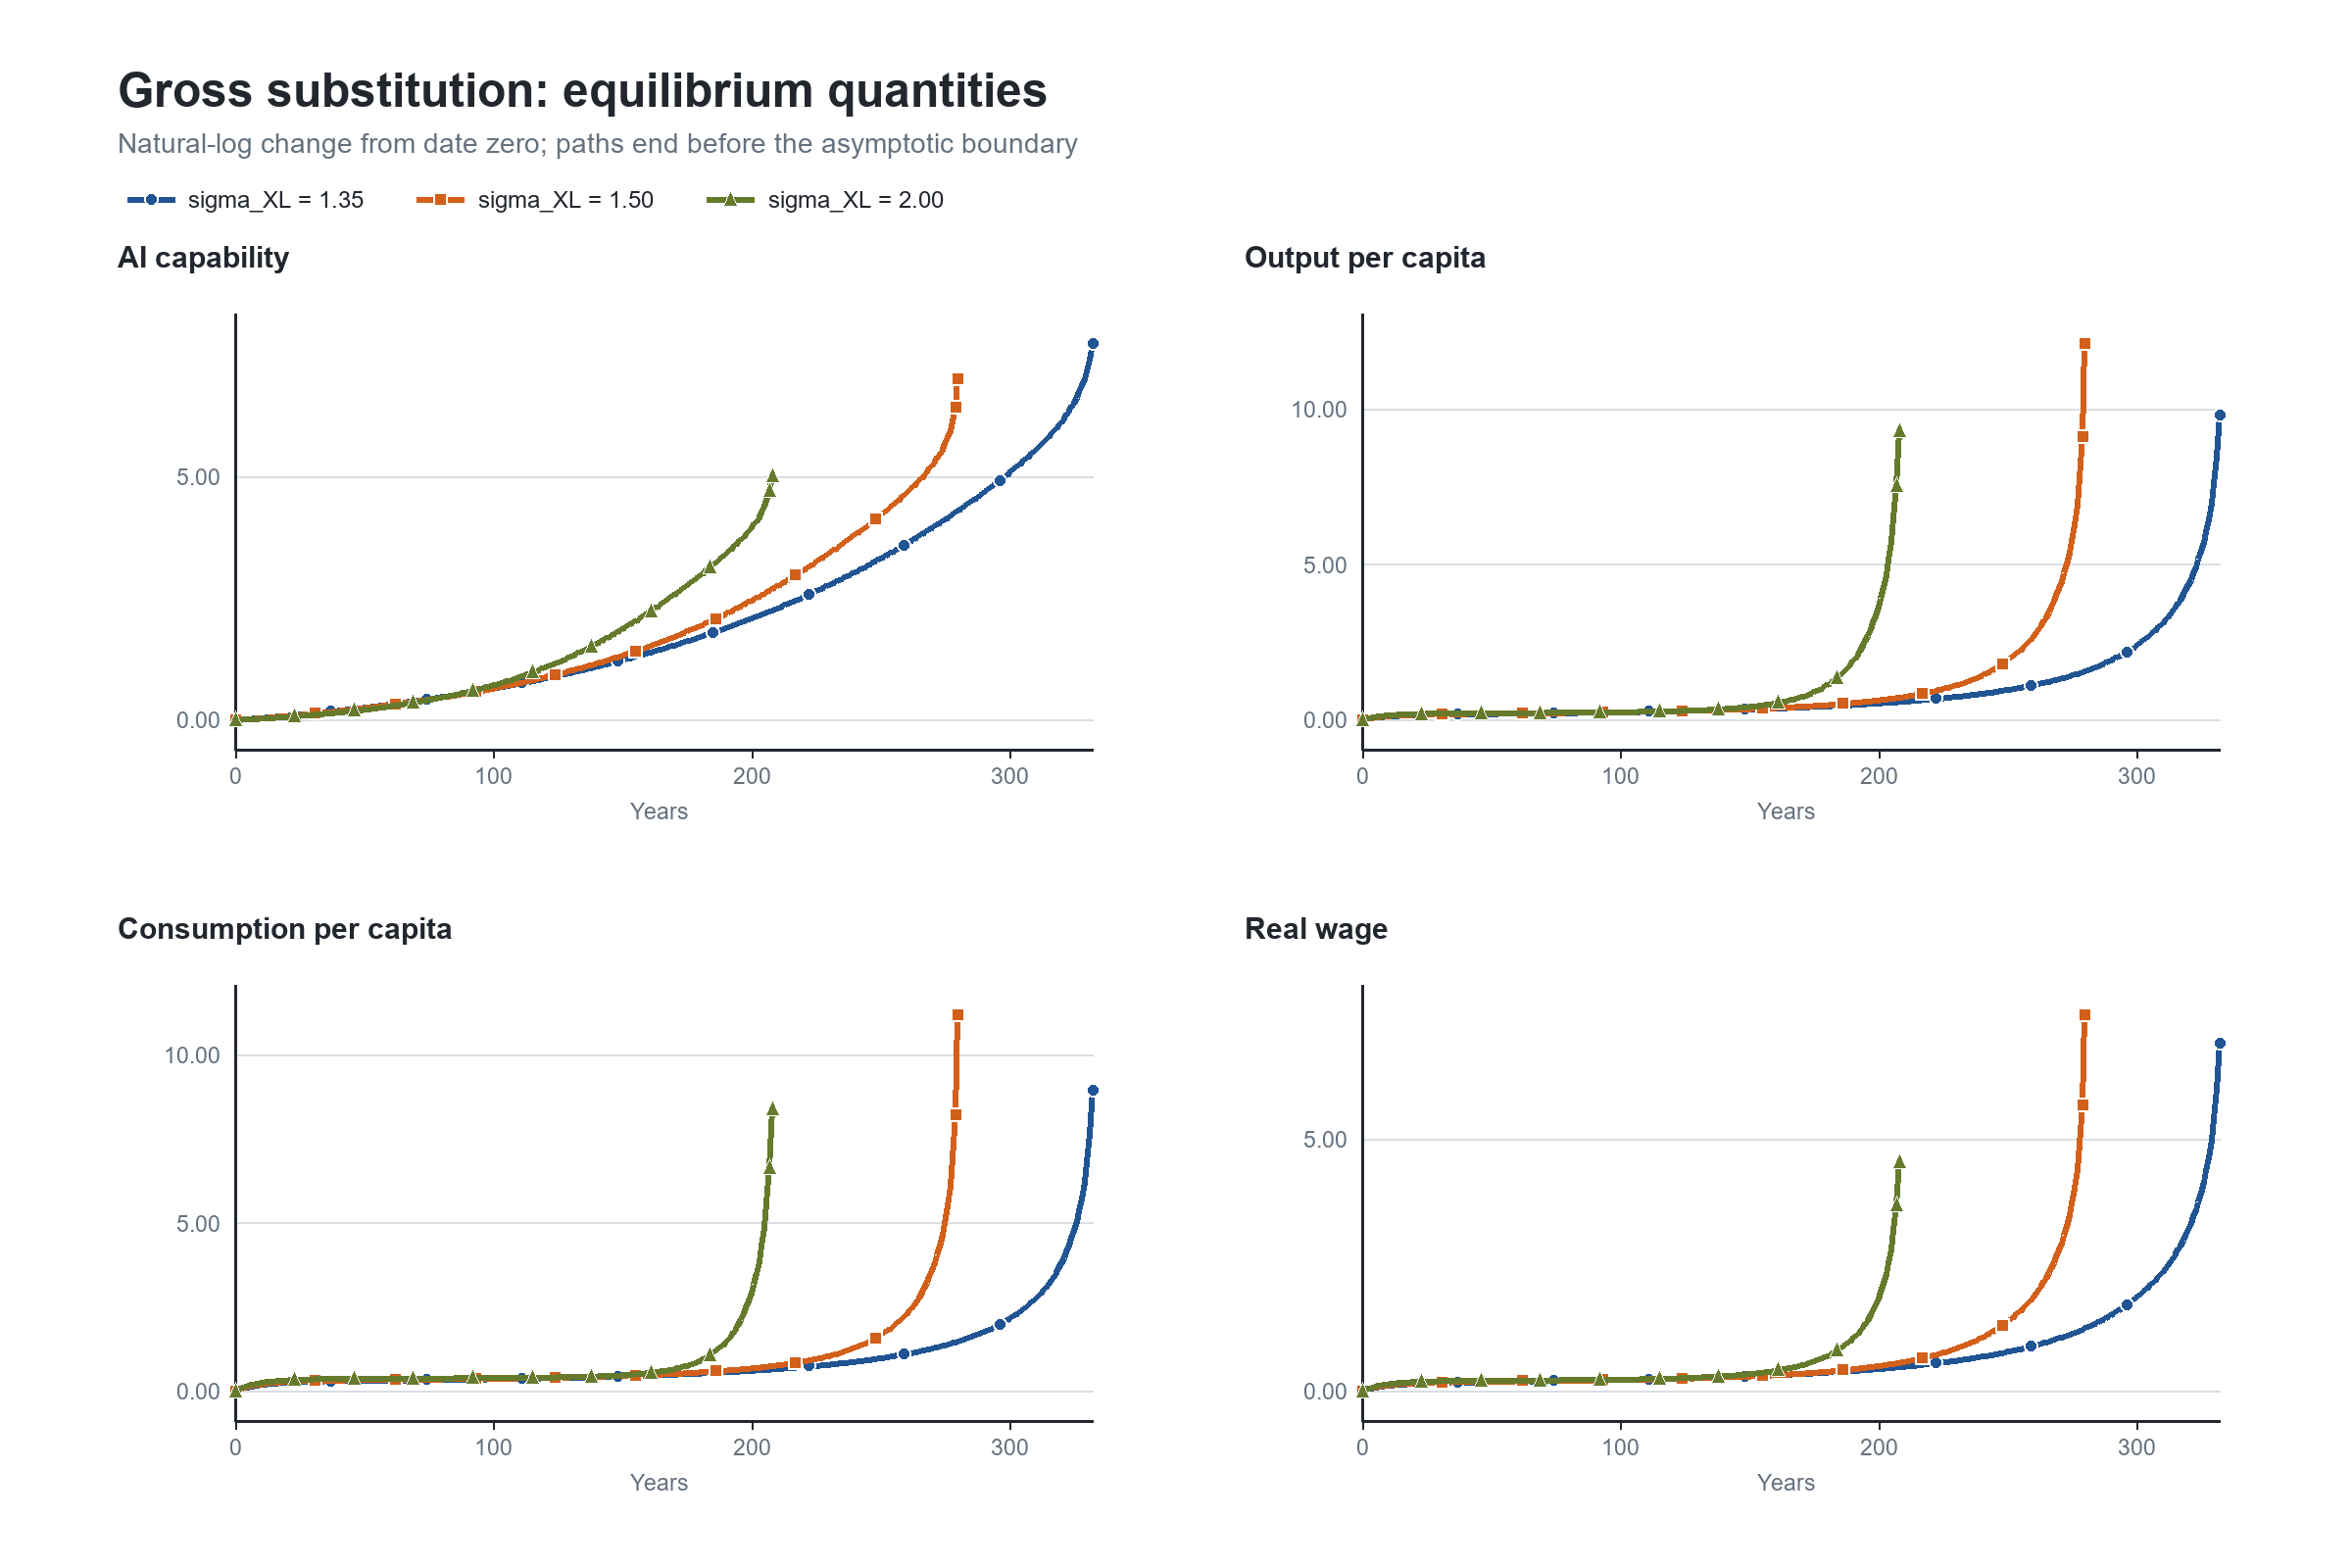
\includegraphics[width=\textwidth]{figures/high_sigma_equilibrium_levels.png}
    \caption{Equilibrium quantities with gross substitution. Each panel reports
    the natural-log change from the path's date-zero value. For
    comparability, the displayed paths end no later than $Y/K=20$.}
    \label{fig:high-sigma-equilibrium-levels}
\end{figure}

The production-chain panels in
Figure~\ref{fig:high-sigma-equilibrium-production-chain} show where the
acceleration originates. Capability growth lowers the marginal resource cost of
AI services, which induces a large expansion of inference compute and an even
larger expansion of AI services. The service composite consequently ceases to be
constrained by labor. The dates differ sharply across elasticities, but the ordering
of the mechanism is the same in all three equilibria.

\begin{figure}[H]
    \centering
    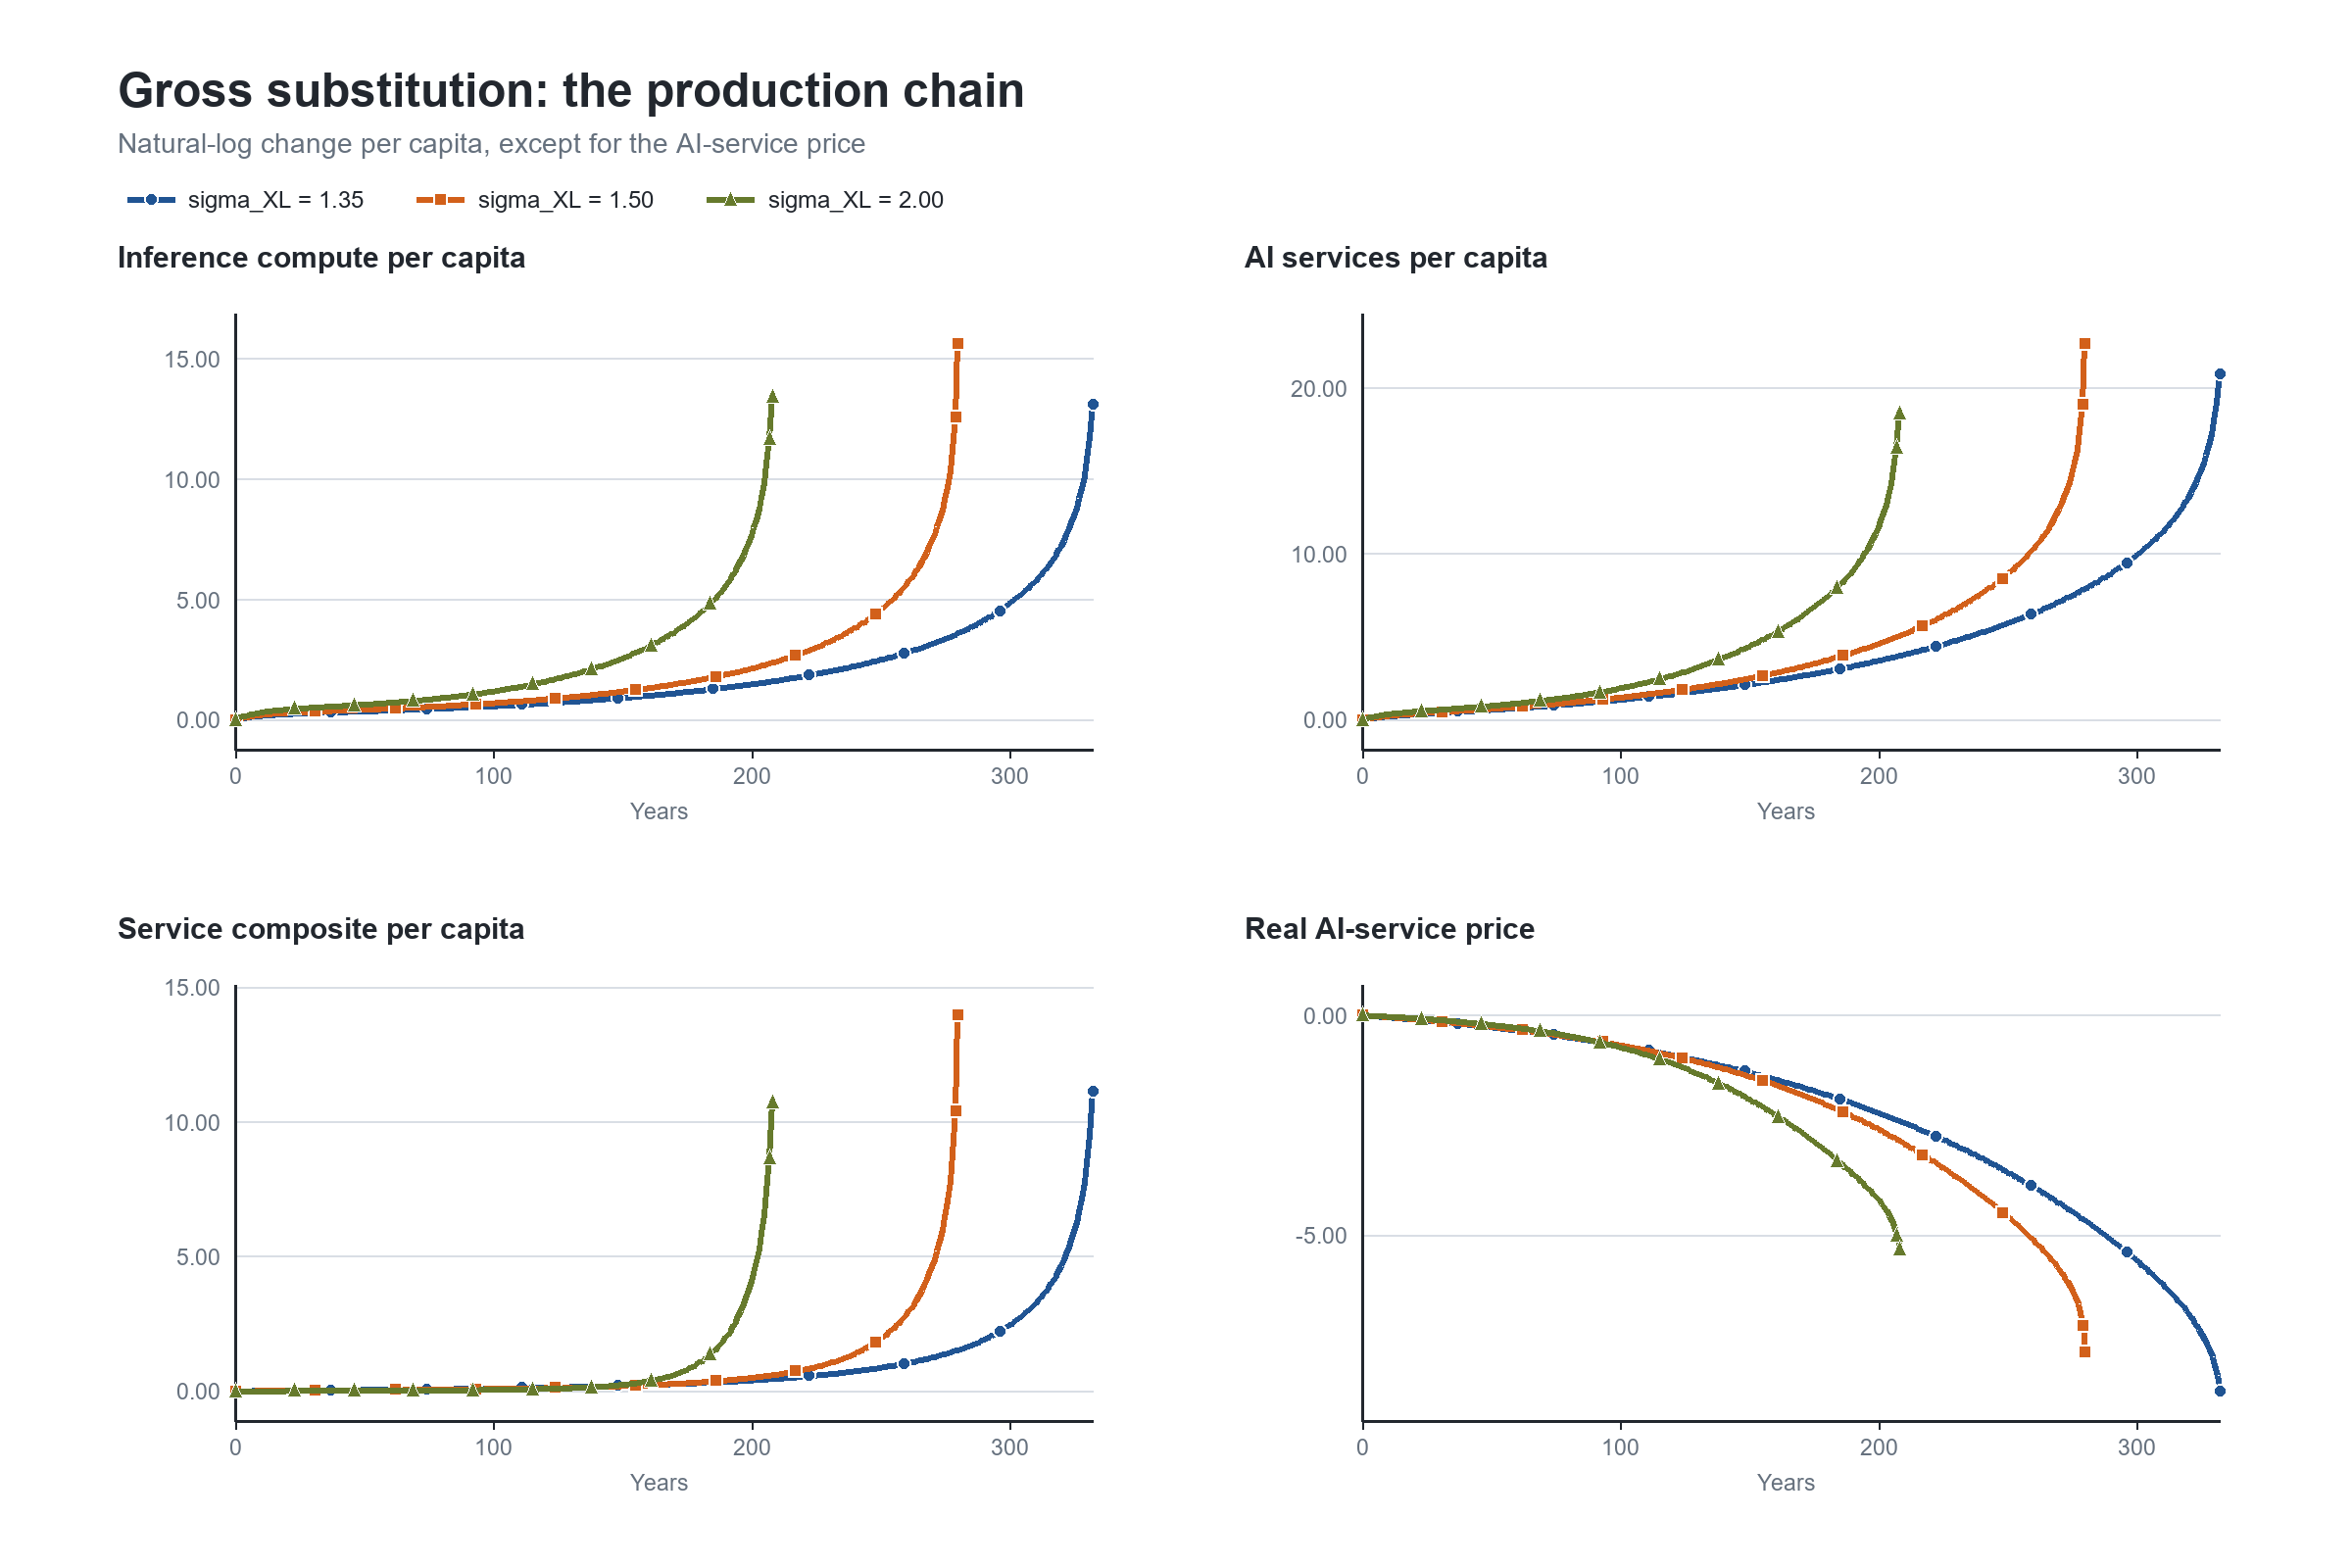
\includegraphics[width=\textwidth]{figures/high_sigma_equilibrium_production_chain.png}
    \caption{Production chain with gross substitution. Quantity panels report
    natural-log changes per capita and the price panel reports a natural-log
    change. Paths are displayed only up to $Y/K=20$.}
    \label{fig:high-sigma-equilibrium-production-chain}
\end{figure}

The growth rates and the return to capital in Figure
\ref{fig:high-sigma-equilibrium-growth} remain comparatively low through most of
the transition and then rise rapidly. Output-per-capita growth first exceeds 5
percent after 297 years when $\sigma_{XL}=1.35$, after 247 years when it is 1.50,
and after 180 years when it is 2.00. The real wage rises throughout all three
paths. The acceleration therefore does not require a falling wage, even though
labor receives a vanishing share of output.

Figure~\ref{fig:high-sigma-equilibrium-monopoly-block} adds the objects that
cannot be inferred from quantities alone. Both the AI-service price and marginal
cost fall, and their decline accelerates. Unlike the complementarity case, the
price moves toward marginal cost: the markup declines toward roughly 1.5 on the
reported boundaries. Operating profits nevertheless rise from a small initial
share to about 22 percent of output. A lower markup can therefore coexist with a
larger aggregate profit share when the AI-service expenditure share expands.
These are equilibrium outcomes for the reported parameterization, not general
comparative-static propositions.

\begin{figure}[H]
    \centering
    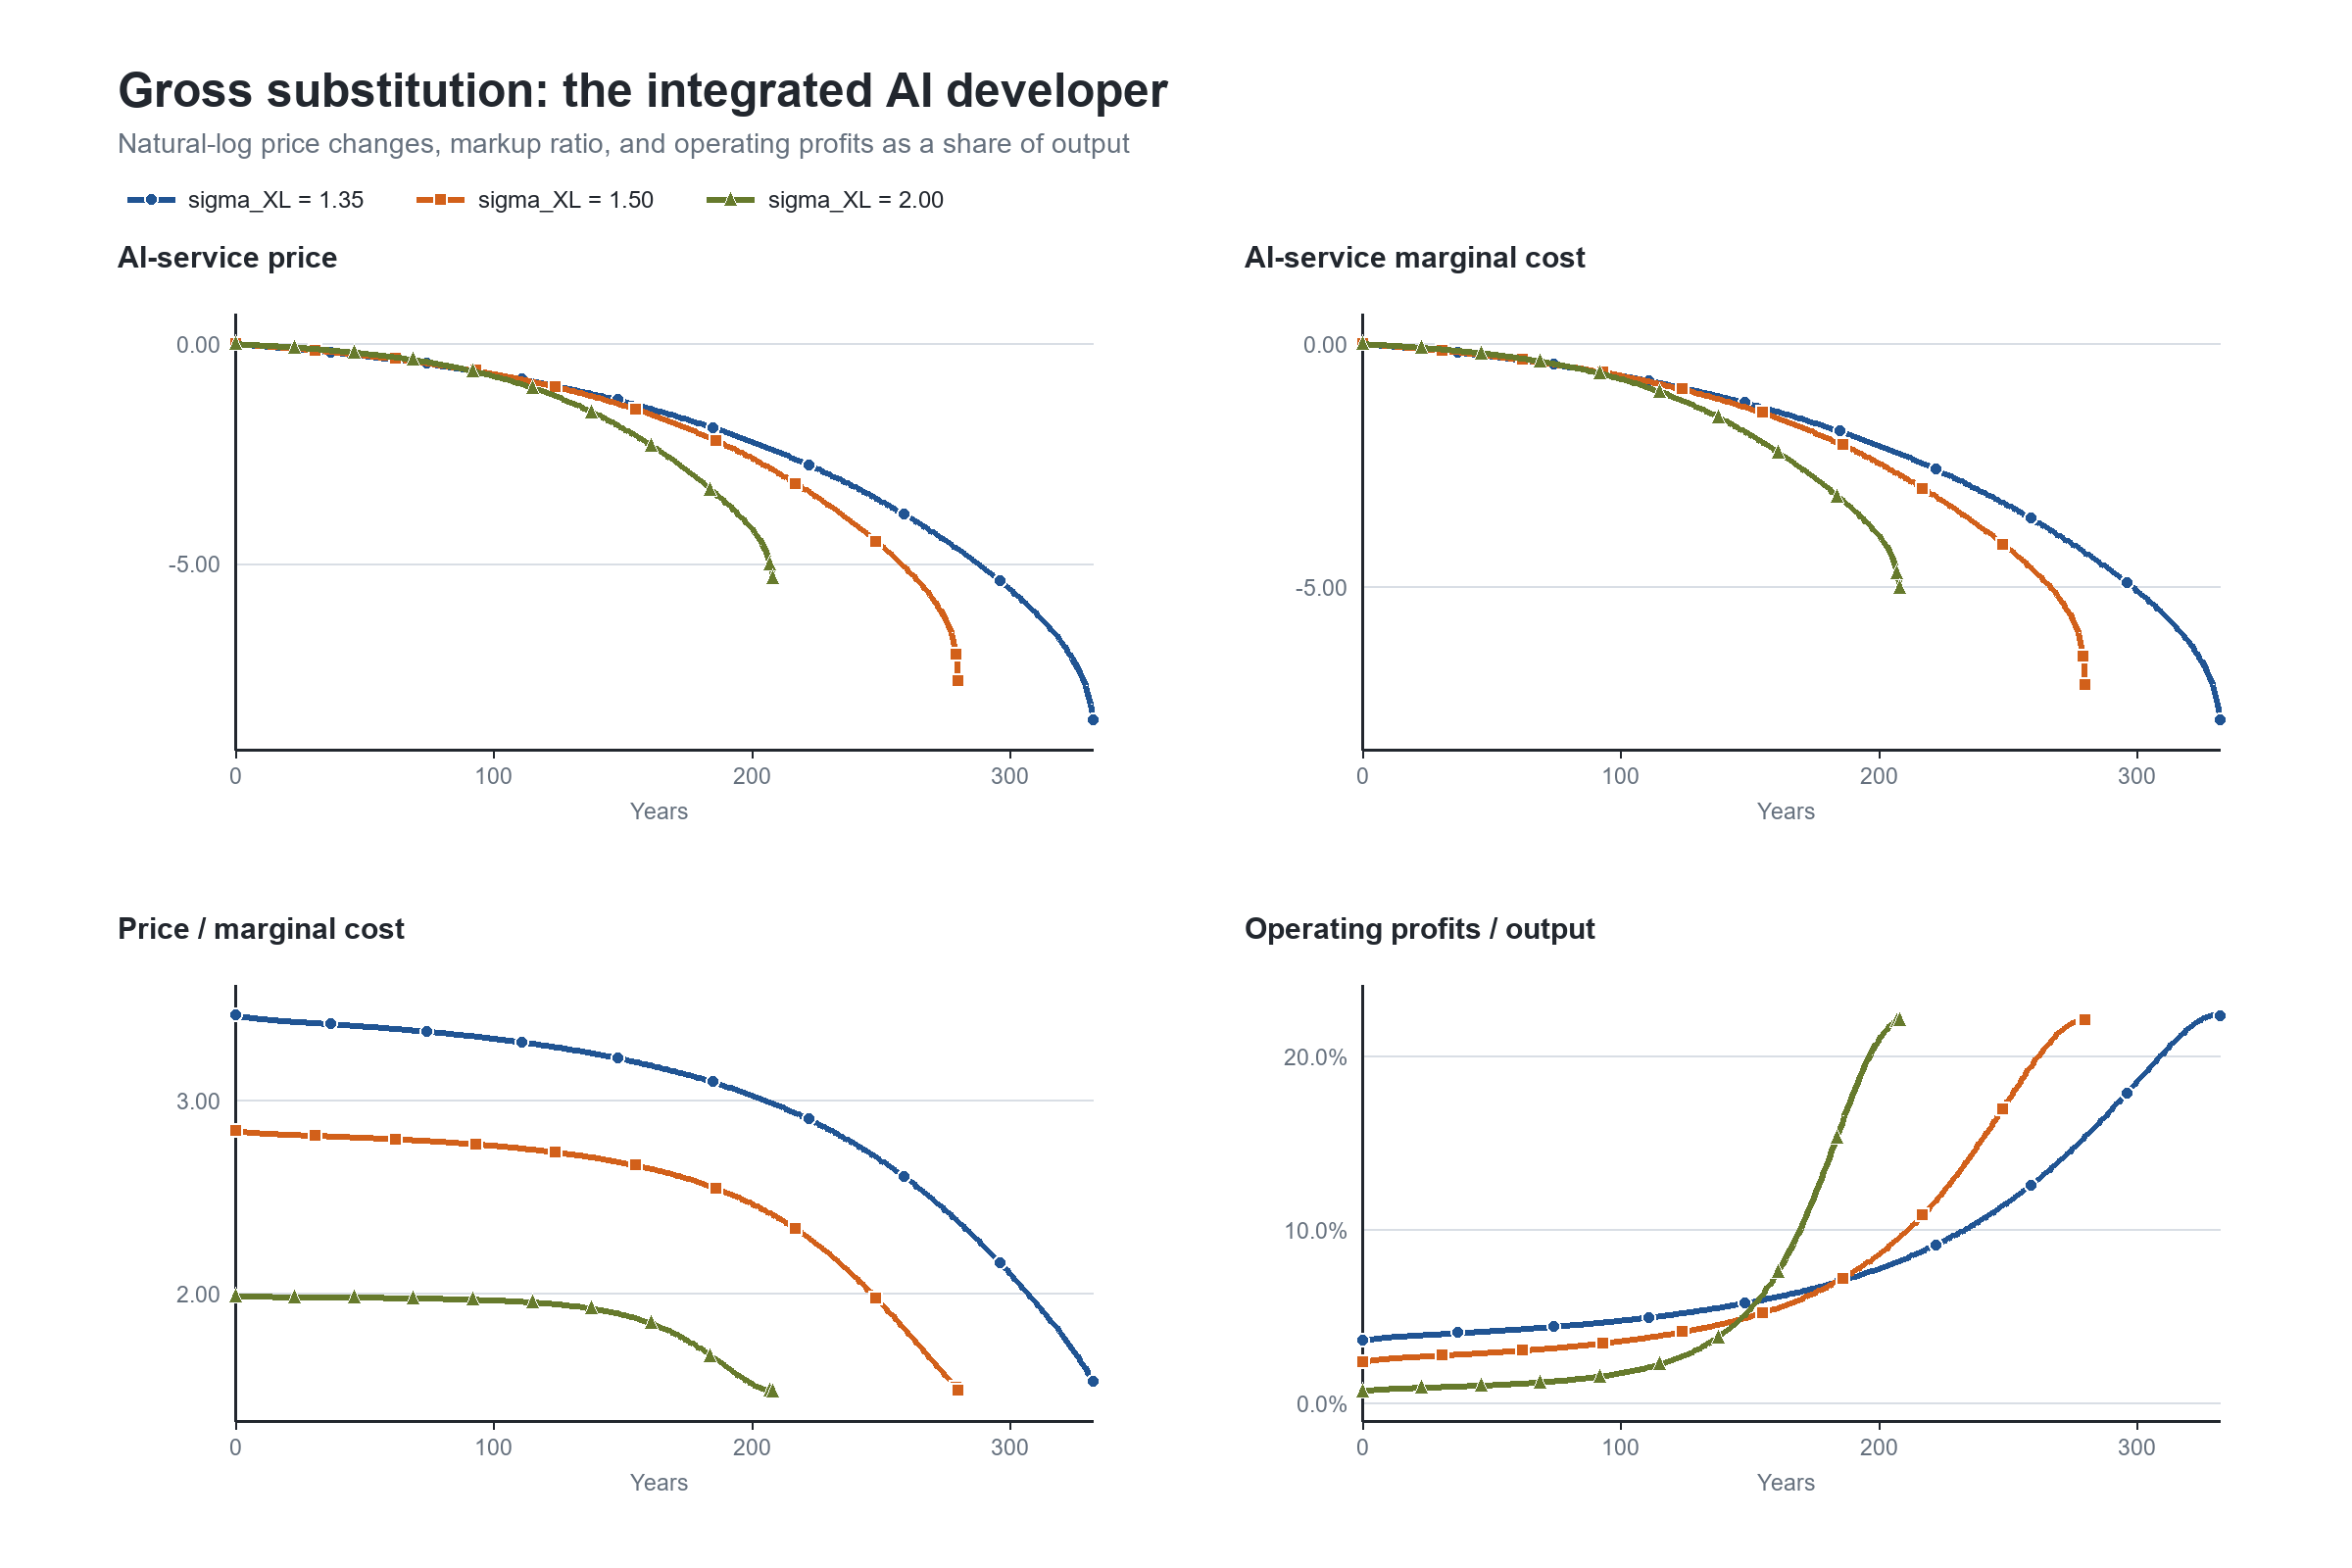
\includegraphics[width=\textwidth]{figures/high_sigma_equilibrium_monopoly_block.png}
    \caption{The integrated AI developer under gross substitution. Price and
    marginal cost are natural-log changes; the markup is a ratio and operating
    profits are a percentage of output.}
    \label{fig:high-sigma-equilibrium-monopoly-block}
\end{figure}

Figure~\ref{fig:high-sigma-equilibrium-shares} separates the production and
research margins. The AI contribution to production and the automated contribution
to research approach one, while the aggregate labor share approaches zero. Human
research employment need not follow the aggregate labor share. With
$\sigma_{XL}=1.35$ and 1.50, $H/N$ rises and later falls as automated research
becomes dominant. With $\sigma_{XL}=2$, the scale of research expands so quickly
that $H/N$ reaches 90.7 percent at the $Y/K=100$ boundary even though automated
systems account for 99.8 percent of effective research. A nearly automated research
technology can therefore employ most humans while paying them a negligible share
of an economy that is growing much faster than wages.

\begin{figure}[H]
    \centering
    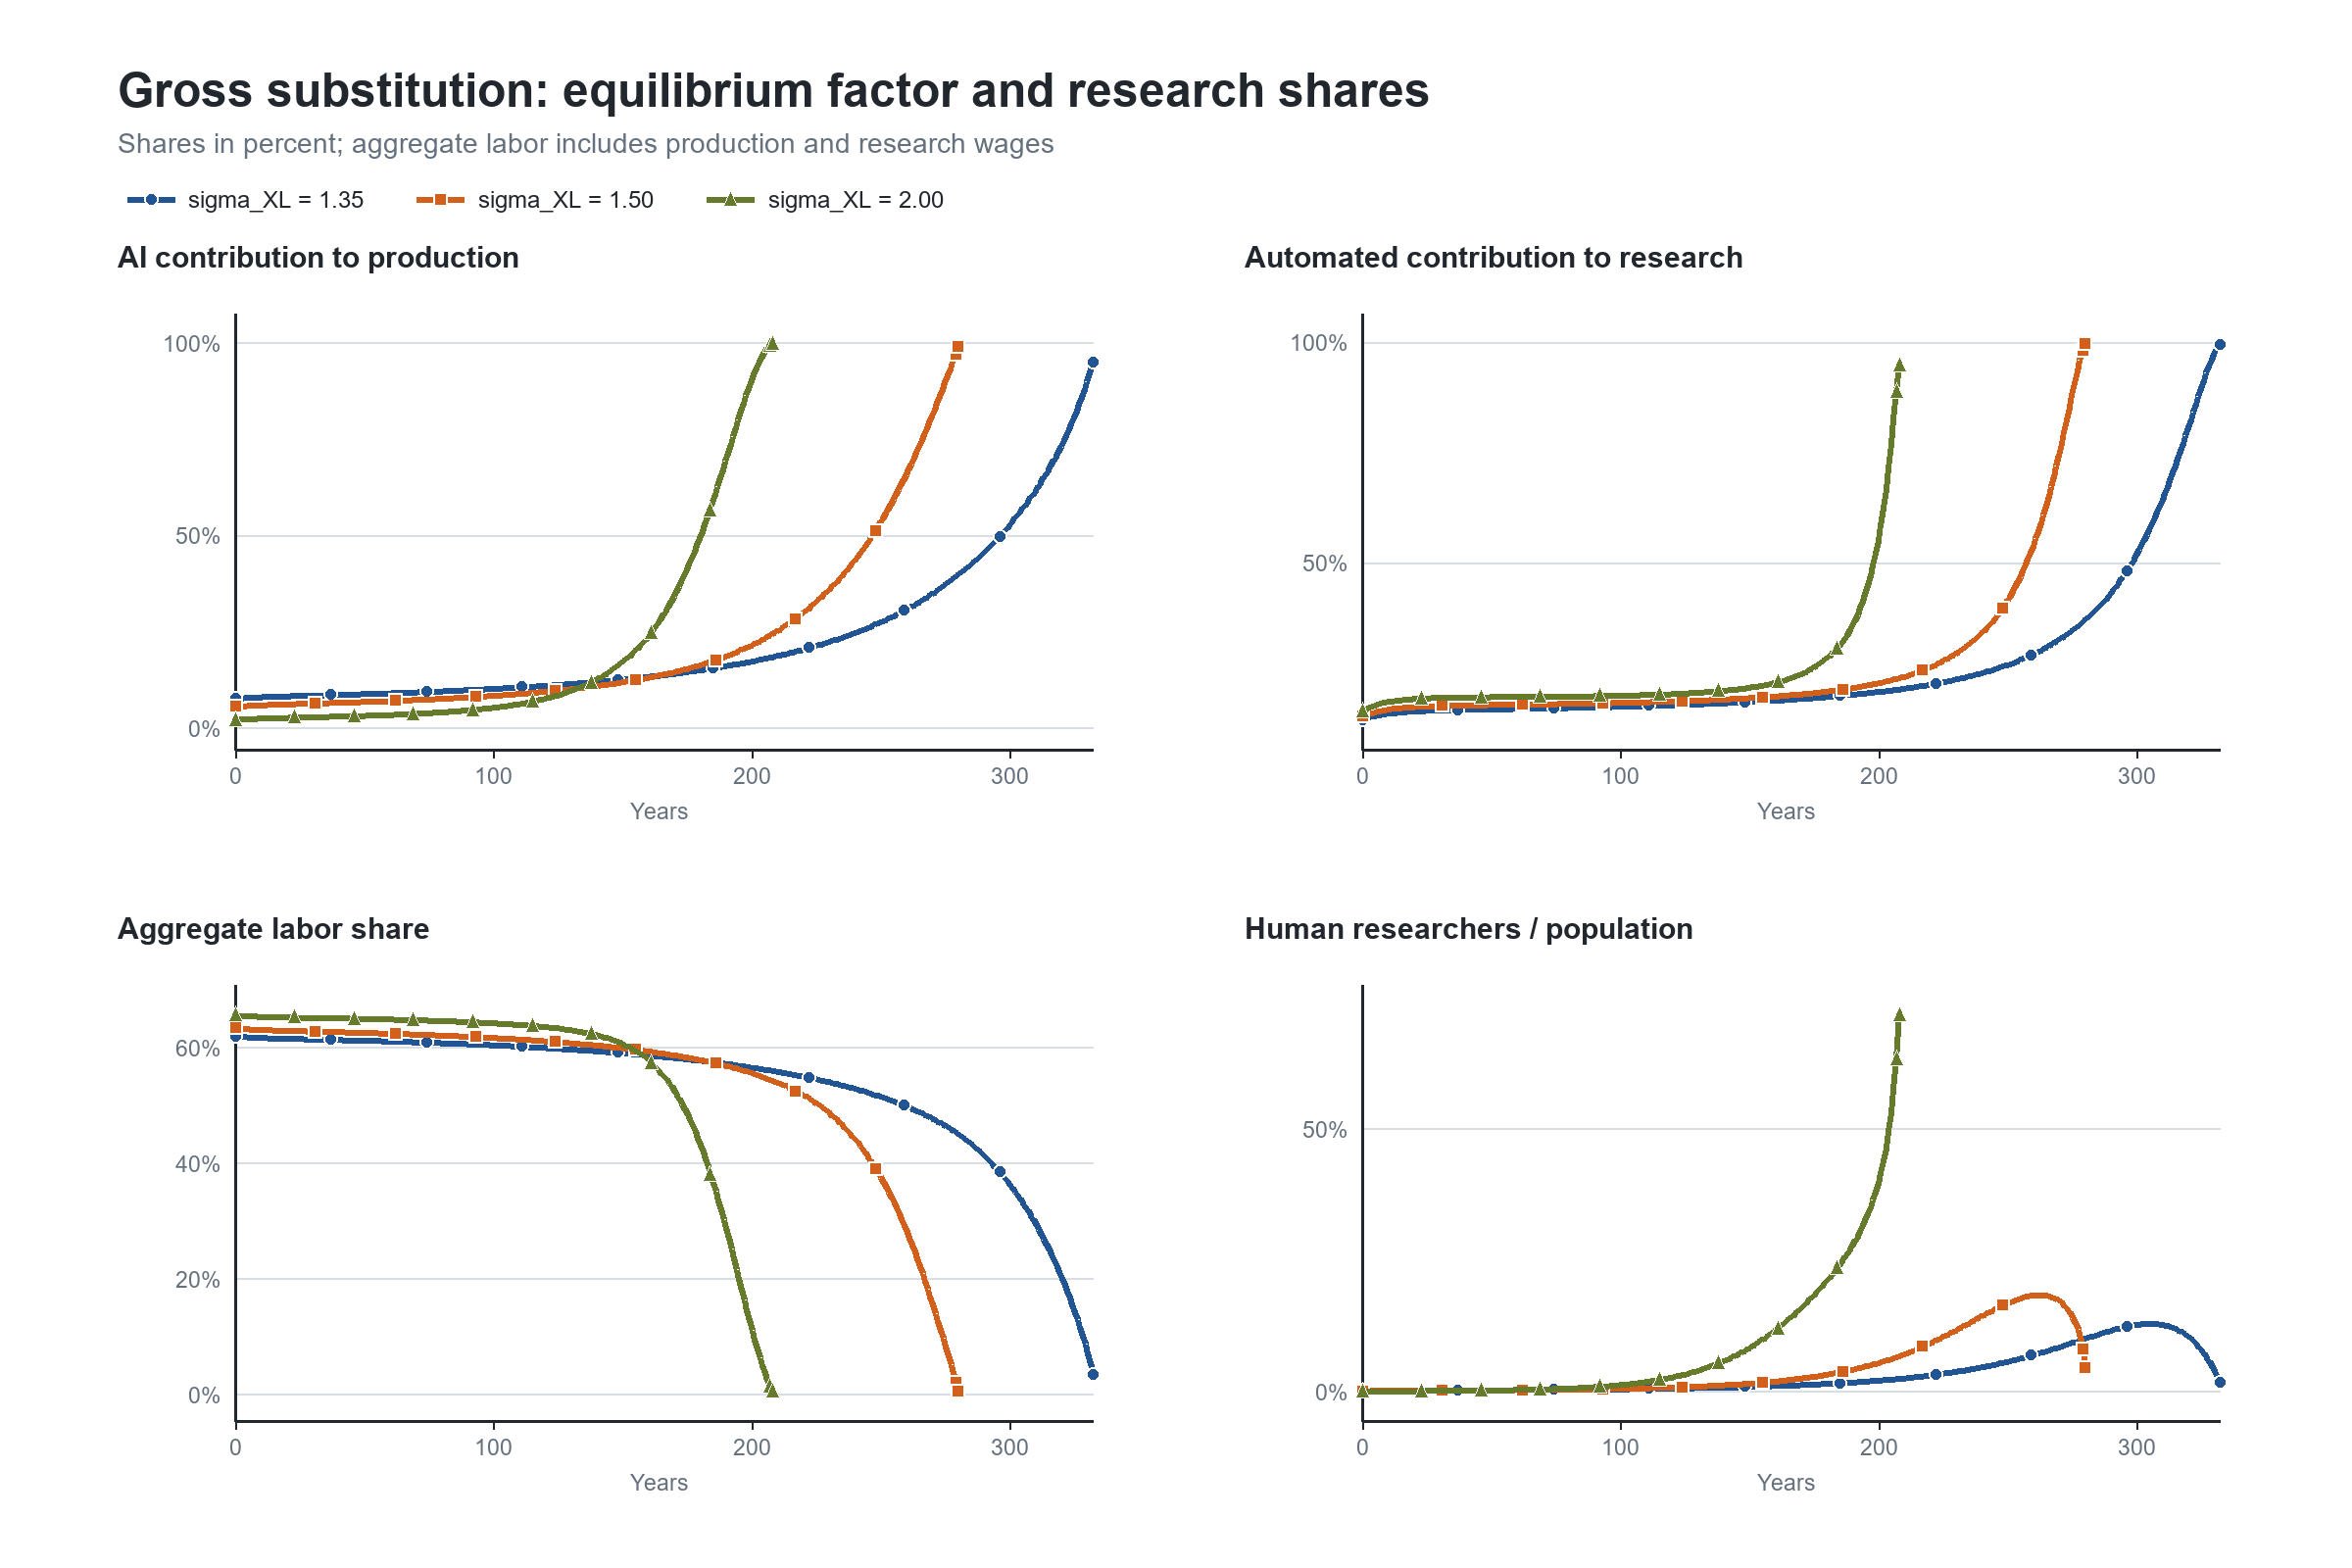
\includegraphics[width=\textwidth]{figures/high_sigma_equilibrium_shares.png}
    \caption{Production, research, and labor allocation along the gross-substitution
    equilibria. The aggregate labor share includes production and research wages.}
    \label{fig:high-sigma-equilibrium-shares}
\end{figure}

Figure~\ref{fig:high-sigma-equilibrium-research-chain} complements those shares
with levels. Automated and effective research expand rapidly per capita, while
$\ln(H/M)$ falls without reversal. Human research per capita can first rise and
then fall, or keep rising over the computed interval, because its level reflects
both a declining human intensity and an expanding research sector. This is the
numerical counterpart of Proposition~\ref{prop:research-employment-scale}.

\begin{figure}[H]
    \centering
    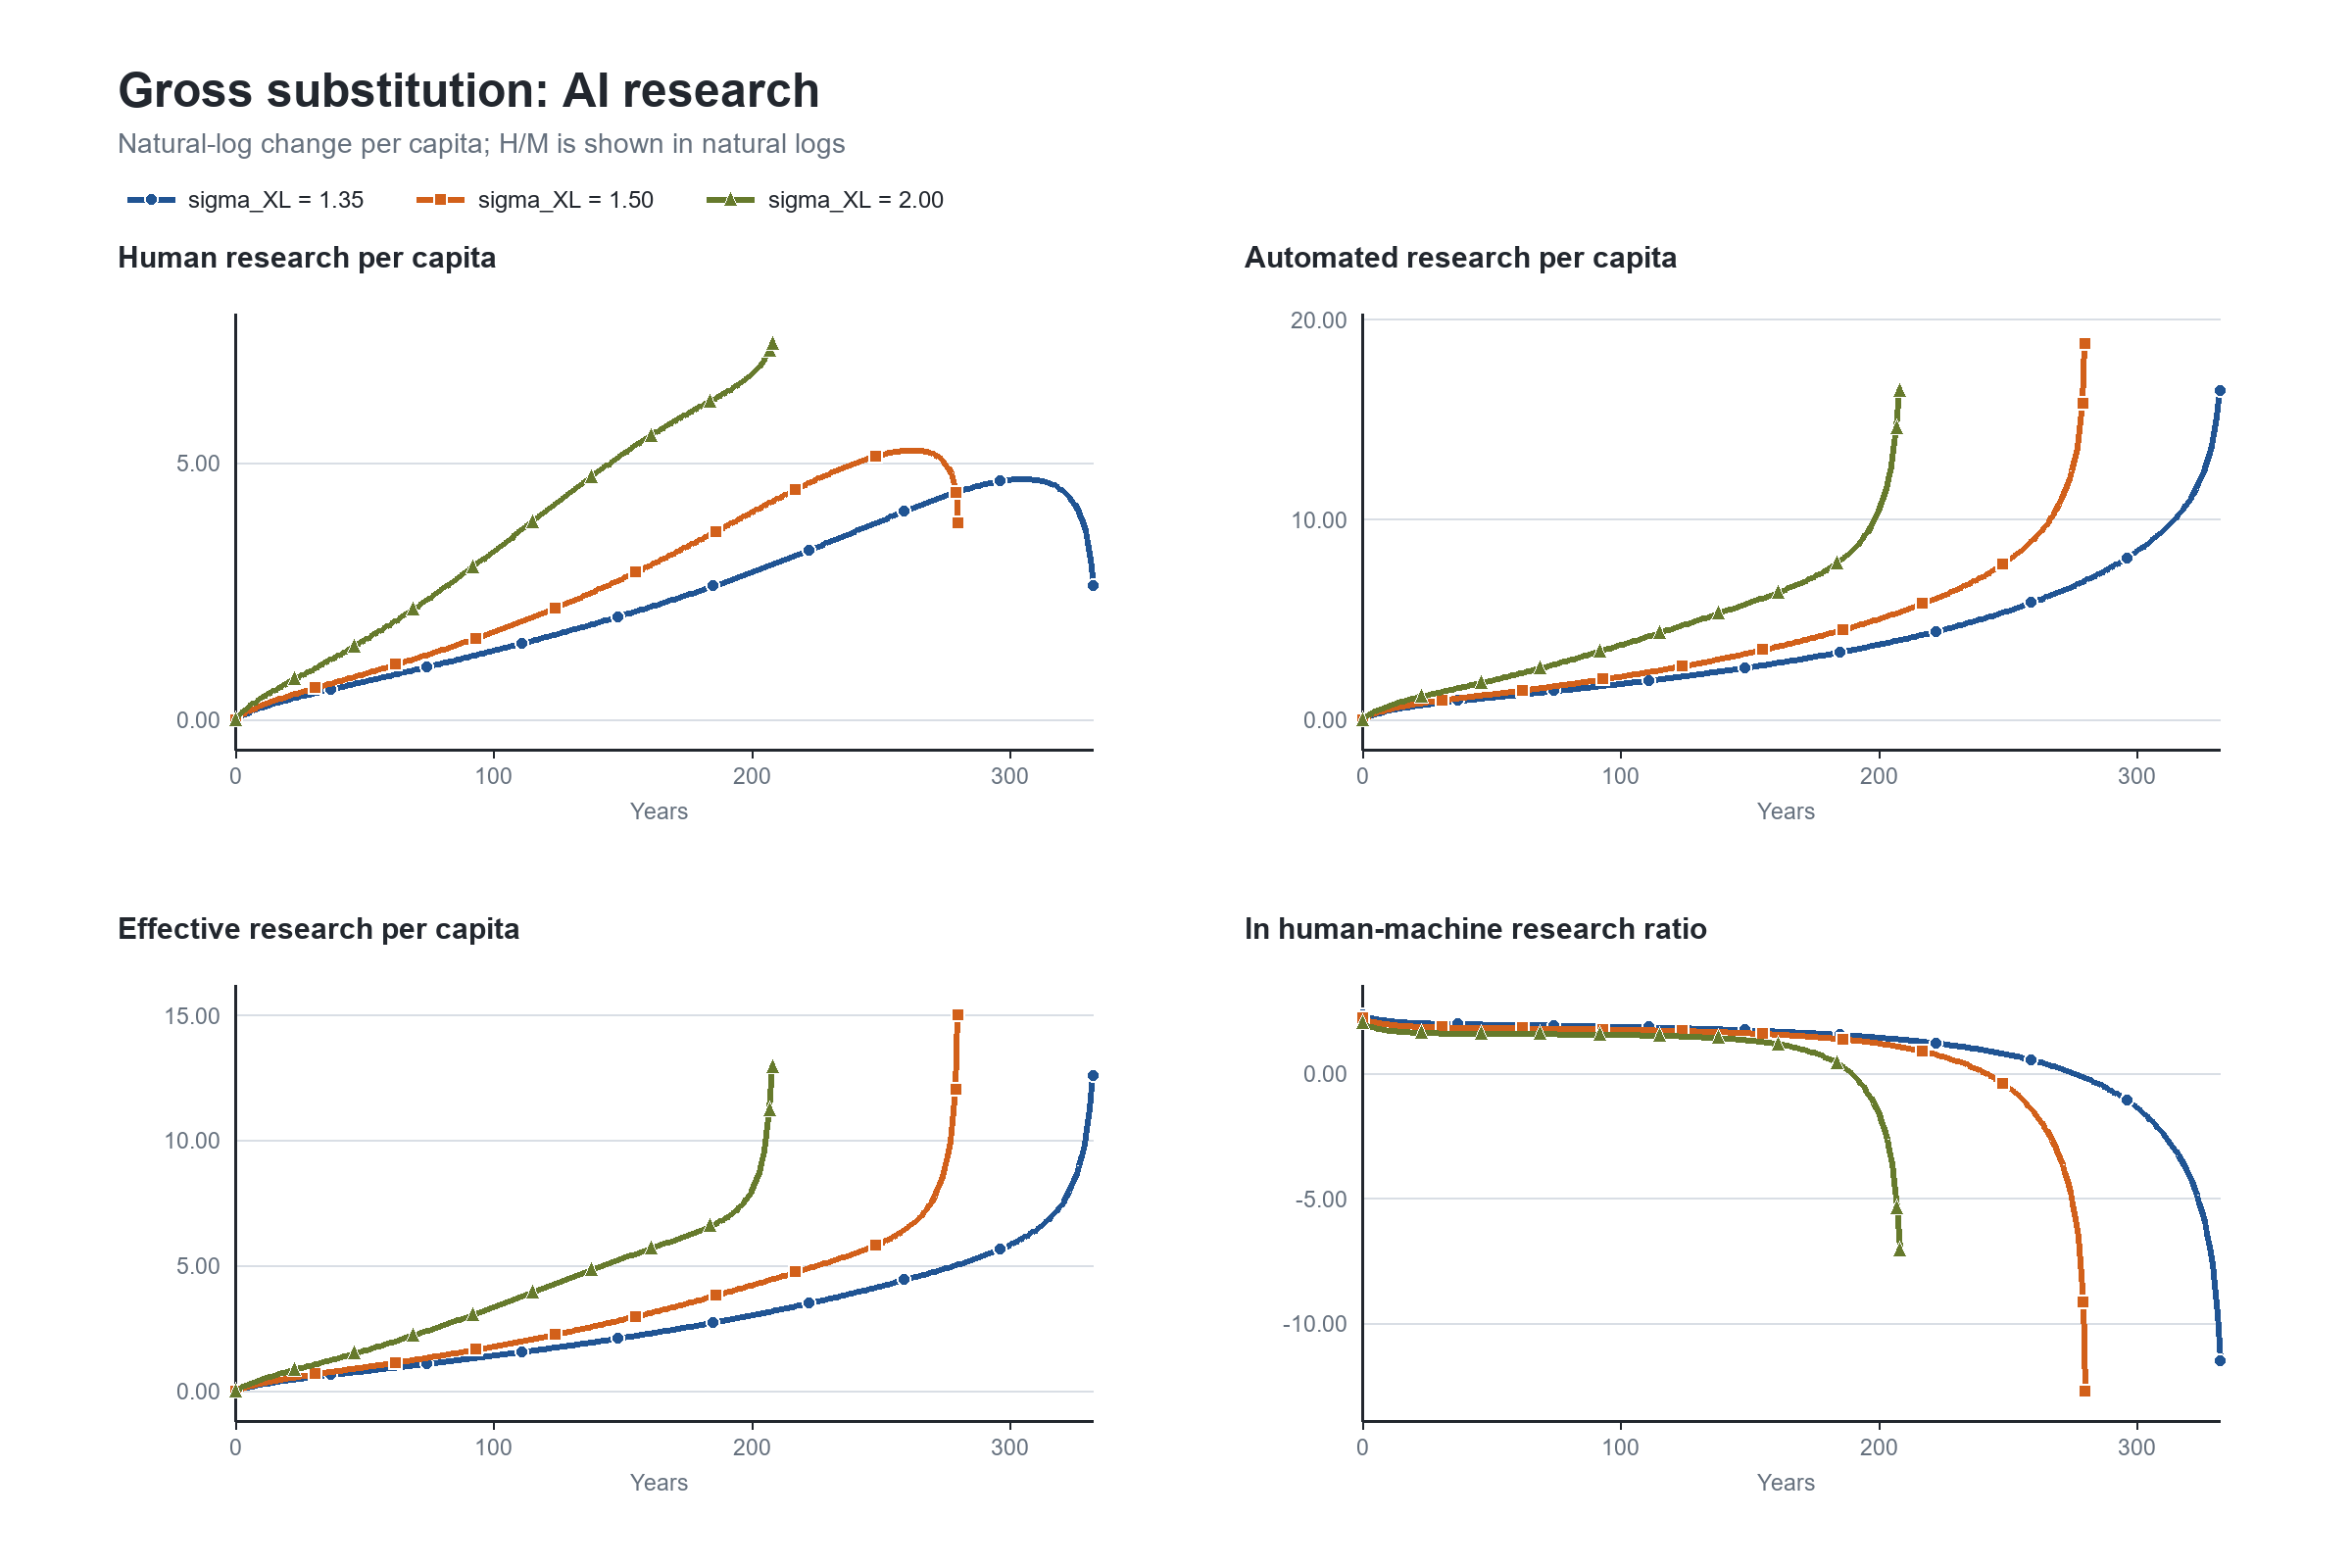
\includegraphics[width=\textwidth]{figures/high_sigma_equilibrium_research_chain.png}
    \caption{Research chain with gross substitution. The first three panels
    report natural-log changes per capita; the final panel reports $\ln(H/M)$.}
    \label{fig:high-sigma-equilibrium-research-chain}
\end{figure}

The resource allocation in
Figure~\ref{fig:high-sigma-equilibrium-resource-allocation} shows that acceleration
is accompanied by a large reallocation of output. Inference absorbs close to 45
percent of output at the terminal boundaries and automated research about 8--9
percent, while consumption falls toward the imposed limiting share. Investment
does not vanish: it remains near 20 percent of output. These shares satisfy the
resource constraint at every plotted date.

\begin{figure}[H]
    \centering
    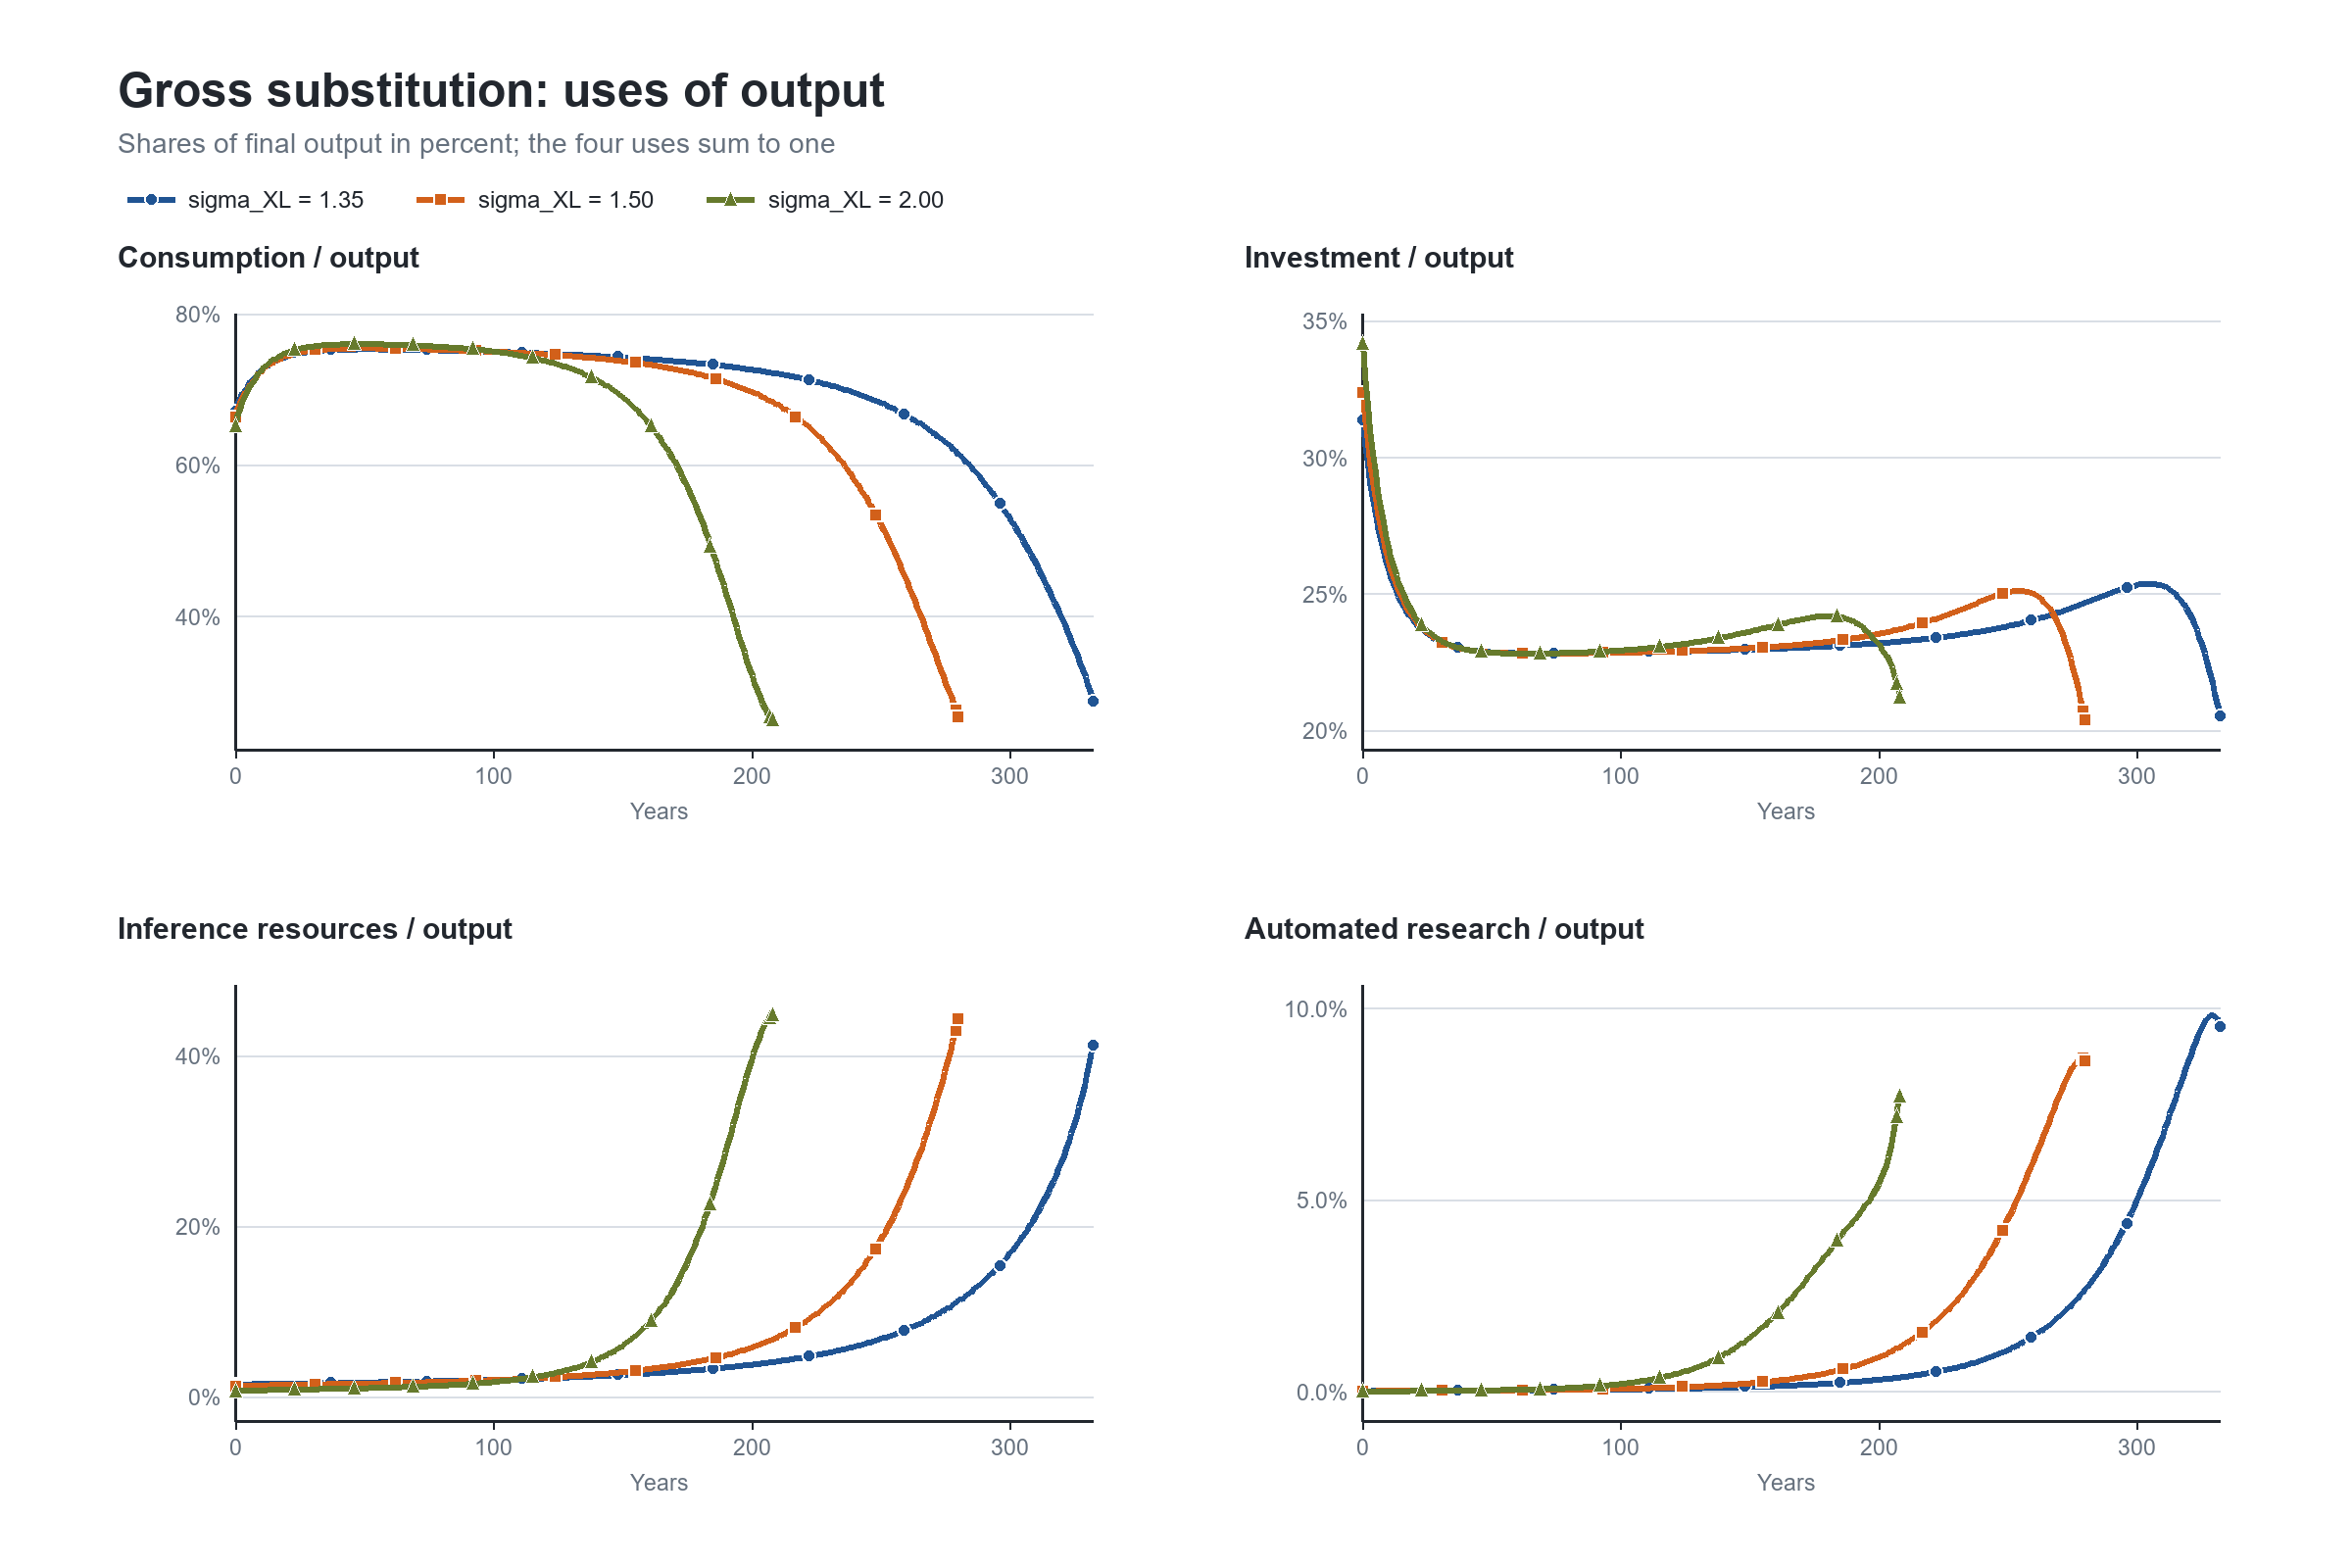
\includegraphics[width=\textwidth]{figures/high_sigma_equilibrium_resource_allocation.png}
    \caption{Allocation of output along the gross-substitution equilibria. Each
    panel is a percentage of final output; the four shares add to one.}
    \label{fig:high-sigma-equilibrium-resource-allocation}
\end{figure}

The boundary tests show that the terminal condition is not driving the transition.
Moving $z_T$ from 20 to 50 changes $\widehat T^*$ from 333.343 to 333.379 years
when $\sigma_{XL}=1.35$ and from 280.436 to 280.450 years when it is 1.50. For
$\sigma_{XL}=2$, moving $z_T$ from 20 to 50 and then to 100 changes
$\widehat T^*$ from 209.079 to 209.076 and 209.075 years. Across these sequences,
initial log consumption changes by less than $2.1\times10^{-8}$ and the initial log
shadow value by less than $3.0\times10^{-5}$.

The boundary directly imposes $C/Y=26.29$ percent and the limiting value of
$qA/K$. Those two ratios are therefore not independent numerical tests of
conditional result~\ref{cond:high-sigma-singular-scaling}. The non-imposed ratio
$g_A/(Y/K)$ approaches its theoretical value of 0.0624. At the largest boundaries,
the investment shares lie between 20.43 and 20.49 percent, compared with the
predicted 20.33 percent, while automated-research resource shares lie between 8.38
and 9.00 percent, compared with the predicted 8.49 percent. These independent
objects provide the relevant numerical check of the singular scaling.

\begin{figure}[H]
    \centering
    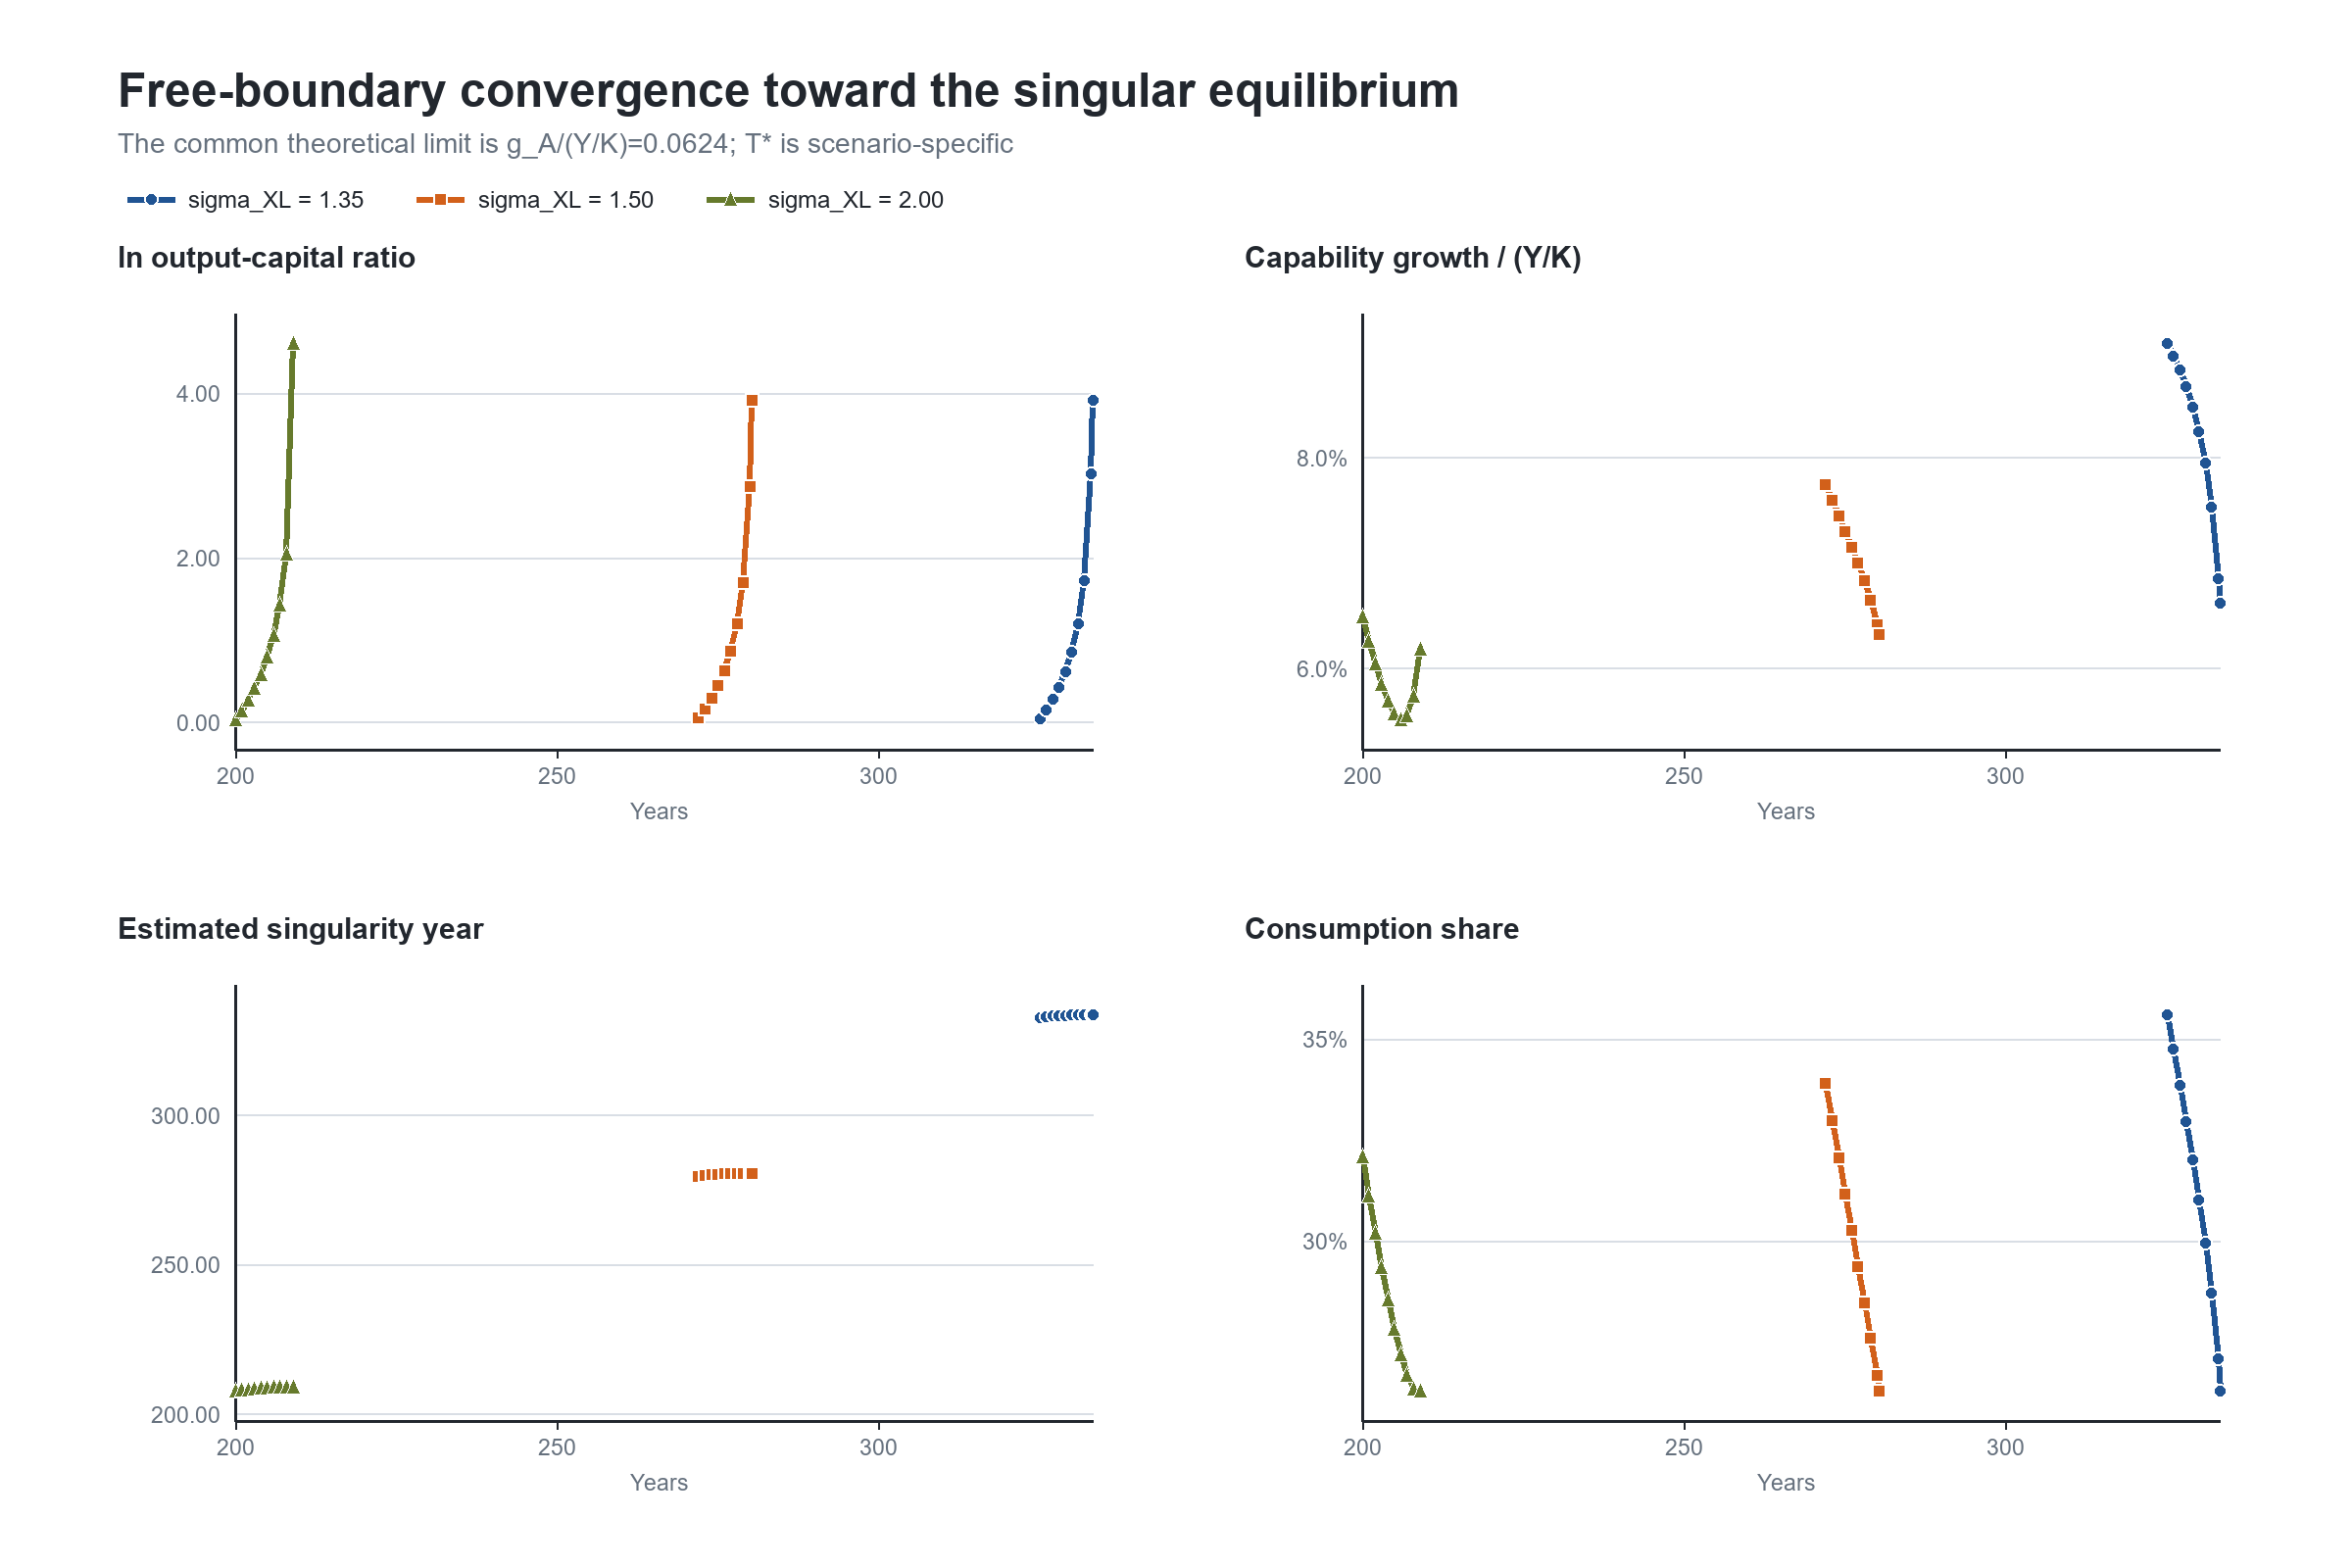
\includegraphics[width=\textwidth]{figures/high_sigma_equilibrium_asymptotics.png}
    \caption{Convergence toward the conditional singular-equilibrium ratios. The
    singularity-date estimator is evaluated only after $Y/K$ reaches one. The
    terminal consumption share is imposed by the free-boundary condition and is
    shown to describe the transition, not as an independent validation moment.}
    \label{fig:high-sigma-equilibrium-asymptotics}
\end{figure}

The maximum collocation residual across the three high-substitution solutions is
$3.0\times10^{-5}$. The largest equation-specific dynamic residual is
$1.7\times10^{-5}$, and the largest static first-order-condition residual is below
$2.0\times10^{-10}$. Labor-market clearing and the aggregate resource constraint
hold to machine precision. These checks establish that the reported curves solve
the numerical equilibrium system on their finite domains. They do not prove global
existence or uniqueness of the limiting singular path.

\subsubsection{Conditional wage-decline search above the static threshold}

The three preceding paths lie below $1/\alpha$, the threshold at which an expansion
of AI services lowers the wage when capital and production labor are held fixed. To
investigate whether the general-equilibrium wage can fall, we extend the numerical
search to $\sigma_{XL}>1/\alpha$ and allow population growth to rise above the
baseline value. Every reported path solves the household Euler equation, the
developer's first-order and costate conditions, the labor market, and the resource
constraint. However, conditional
result~\ref{cond:high-sigma-singular-scaling} establishes the AI-dominated terminal
ratios only for $1<\sigma_{XL}<1/\alpha$. Using those ratios above $1/\alpha$ is an
extrapolative boundary condition. The resulting objects are therefore conditional
equilibrium-branch searches on finite domains, not proofs of global existence or
selection of the terminal branch.

Table~\ref{tab:wage-decline-equilibrium-search} separates three wage outcomes. A
negative minimum value of $g_w$ establishes that the wage falls during part of the
transition. The peak-to-trough decline measures the cumulative fall from the wage's
previous maximum. The final column compares the trough with the wage at date zero.
These measures distinguish a temporary decline from a collapse of the wage level.

\begin{table}[htbp]
    \centering
    \caption{Conditional equilibrium-branch search for wage declines}
    \label{tab:wage-decline-equilibrium-search}
    \begin{tabular}{cccccc}
        \toprule
        $\sigma_{XL}$ & $n$ & $z_T$ & $\min_t g_w$
        & peak--trough decline & trough relative to $w_0$ \\
        \midrule
        4.00 & 1.2\% & 3  &  0.026\% & 0.00\% & 0.00\% \\
        5.00 & 3.0\% & 3  & $-0.216\%$ & 2.22\% & 28.04\% \\
        6.20 & 3.0\% & 10 & $-0.626\%$ & 7.68\% & 21.24\% \\
        6.28 & 3.9\% & 50 & $-0.800\%$ & 9.39\% & 16.72\% \\
        \bottomrule
    \end{tabular}
    \begin{minipage}{0.96\textwidth}
    \footnotesize\emph{Notes:} Except for $\sigma_{XL}$ and $n$, the paths use the
    common parameters and initial stocks in
    Table~\ref{tab:equilibrium-numerical-parameters}. The peak--trough decline is
    reported as a positive percentage. A positive value in the last column means
    that the trough remains above the date-zero wage. Population growth remains
    below the household discount rate, $\rho=4$ percent.
    \end{minipage}
\end{table}

The selected branches produce temporary wage declines but no wage collapse. The wage never falls
when $\sigma_{XL}=4$ and $n=1.2$ percent. When $\sigma_{XL}=5$ and $n=3$ percent,
wage growth becomes negative and the wage falls 2.22 percent from its previous peak.
The decline reaches 7.68 percent when $\sigma_{XL}=6.2$ and 9.39 percent when
$\sigma_{XL}=6.28$ and $n=3.9$ percent. Even in the last configuration, the trough
remains 16.72 percent above the initial wage. All three paths with negative wage
growth subsequently recover.

Figure~\ref{fig:equilibrium-wage-decline-search} shows why the wage and labor's
share need not move together. During the declining phase, rapid AI-service growth
and a production elasticity above $1/\alpha$ make the second term in
equation~\eqref{eq:dynamic-wage-decomposition} negative. Later, capital deepening
raises the first term. At the same time, the expansion of AI research moves workers
out of final production. Production labor becomes scarce even though automated
systems account for a growing contribution to effective research. The wage then
recovers while the aggregate labor share continues to fall.

\begin{figure}[htbp]
    \centering
    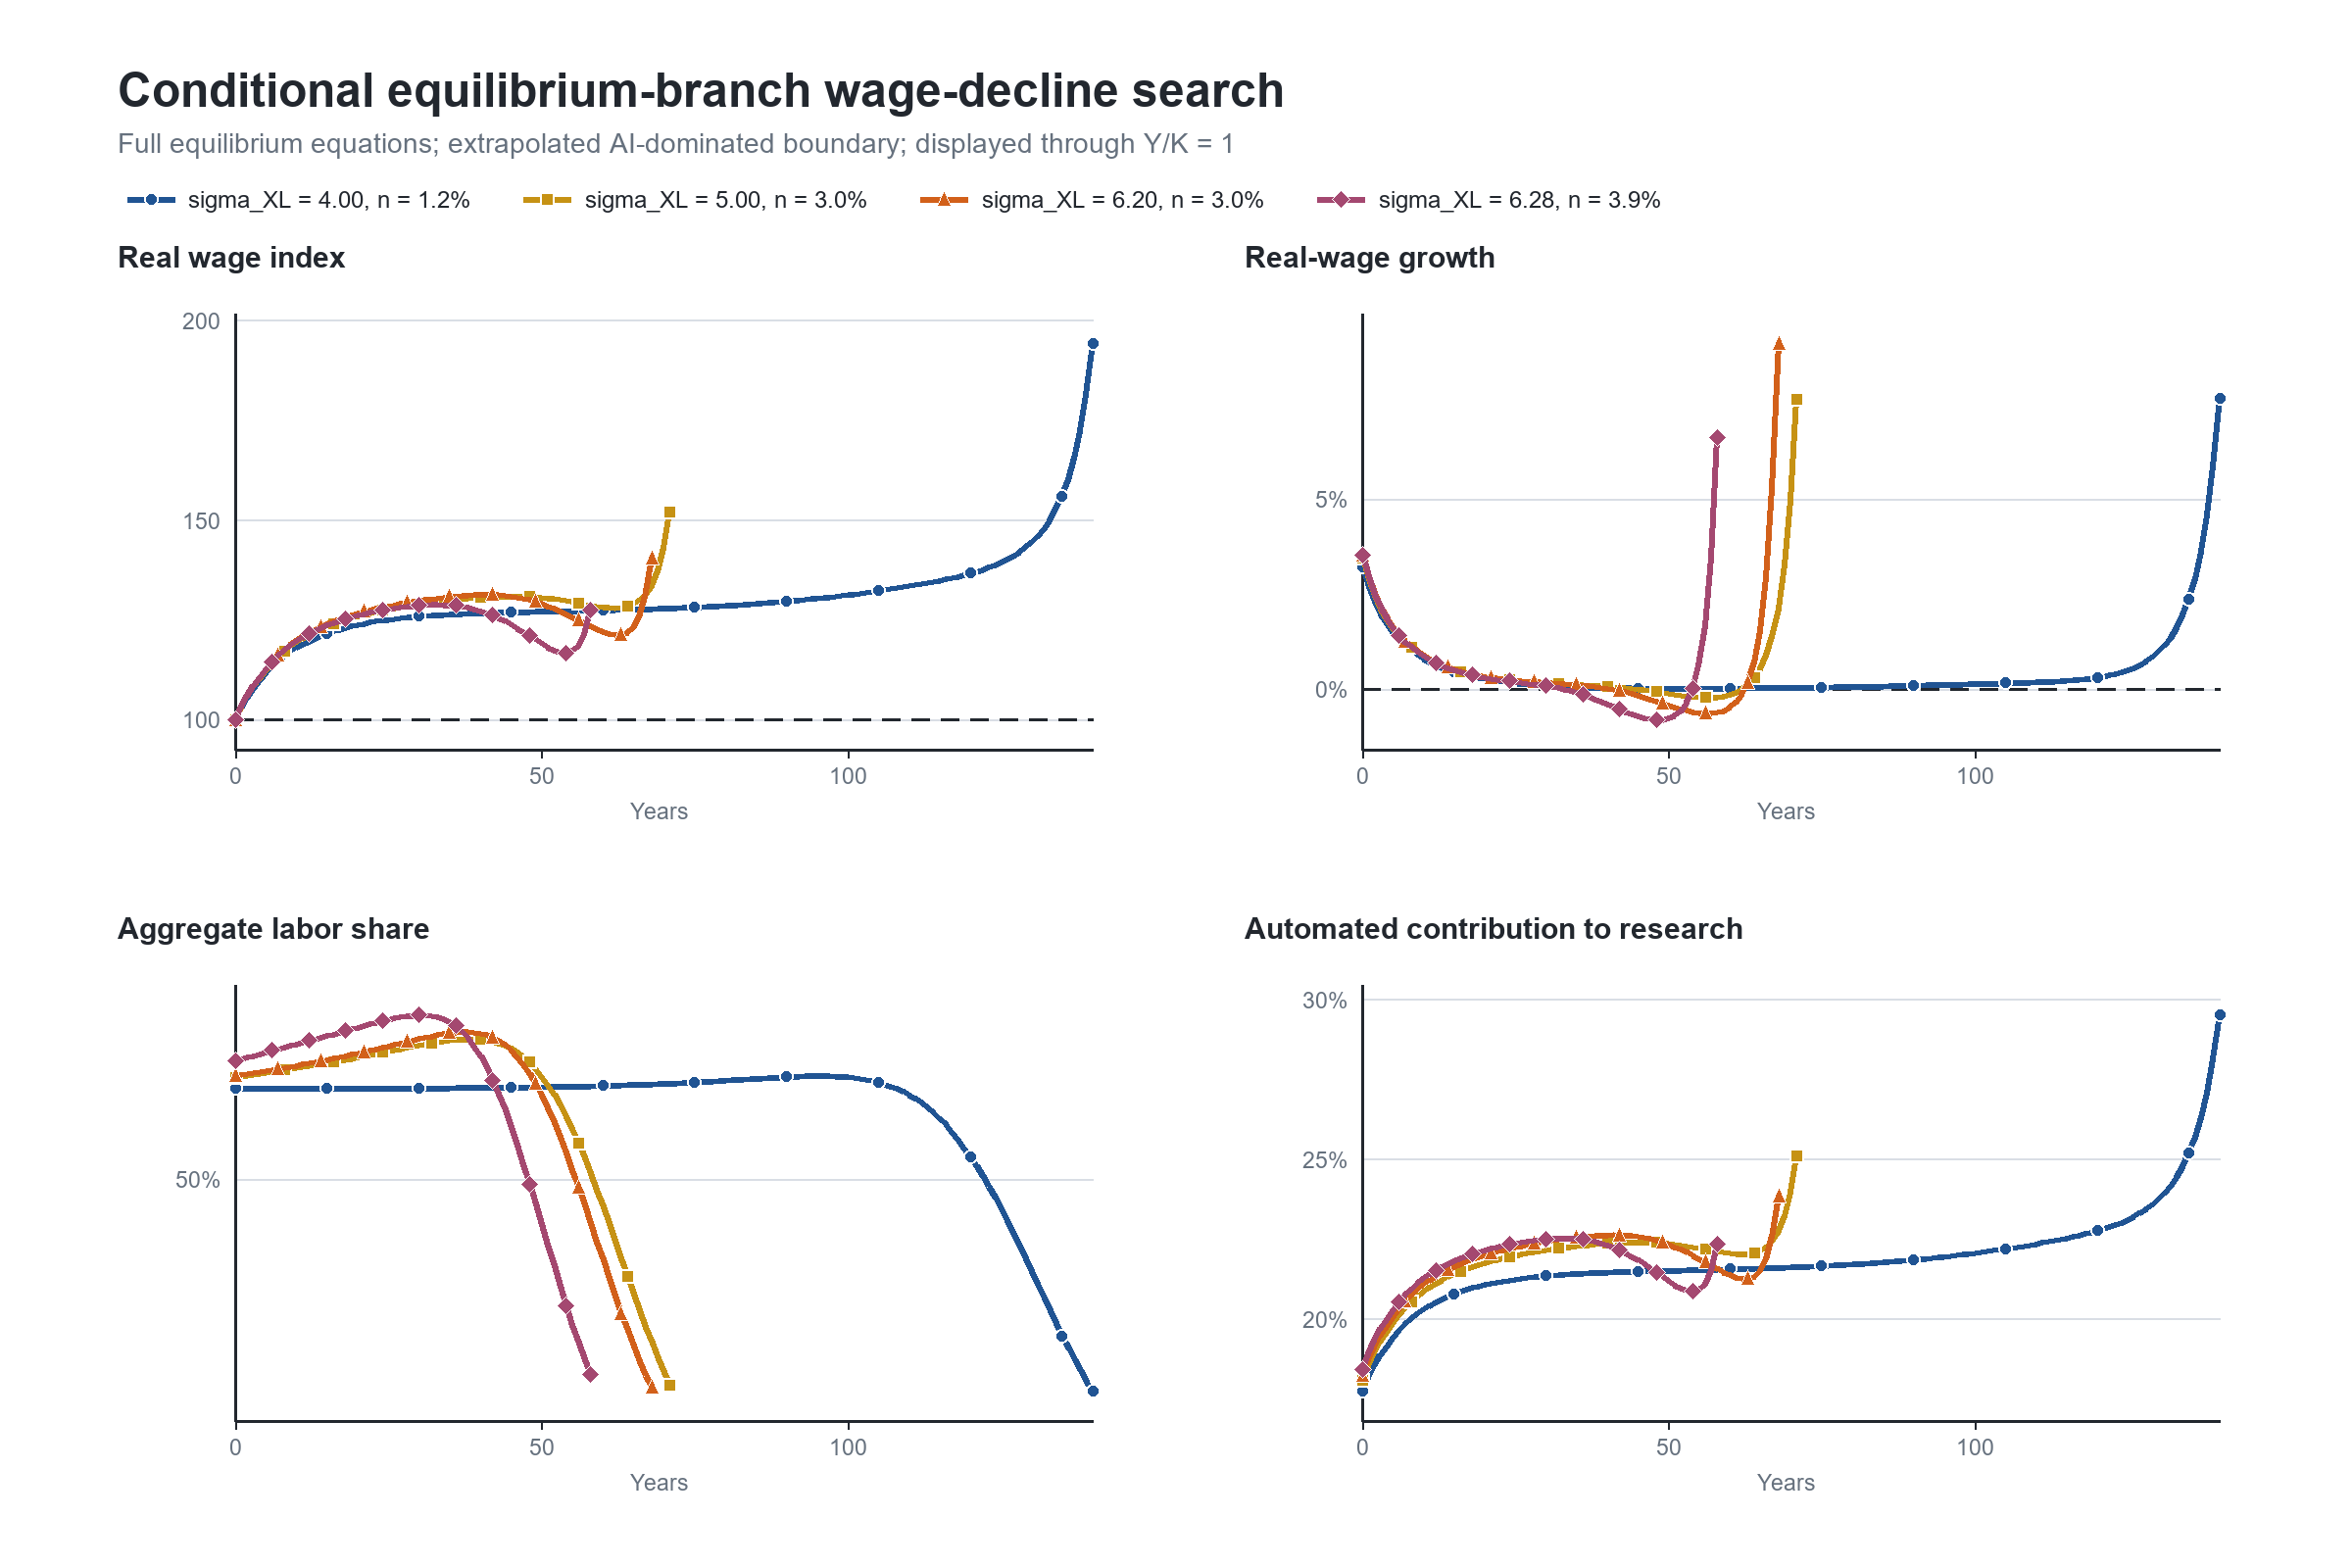
\includegraphics[width=\textwidth]{figures/equilibrium_wage_decline_search.png}
    \caption{Conditional equilibrium-branch search for wage declines. The wage
    index equals 100 at date zero. Growth rates and shares are percentages. The
    displayed transition ends when $Y/K$ reaches one so that the temporary wage
    decline remains visible. The aggregate labor share includes human researchers.}
    \label{fig:equilibrium-wage-decline-search}
\end{figure}

Proposition~\ref{prop:automated-research-wage} supplies an analytical sufficient
condition for eventual recovery: automated research per capita must diverge. The
conditional singular branch in result~\ref{cond:high-sigma-singular-scaling}
satisfies this condition in the parameter region covered by that result. The
wage-decline searches use still higher production elasticities and an extrapolated
terminal boundary, so their recovery remains numerical evidence rather than an
unconditional theorem for every admissible equilibrium. In these paths, the human
research share of population approaches one over the computed transition and
production labor becomes scarce. Moving the terminal value of $Y/K$ from 3 to 10
when $\sigma_{XL}=6.2$ changes the largest pre-year-60 difference in log wages by
0.0015. Moving it from 10 to 50 when $\sigma_{XL}=6.28$ changes the largest
pre-year-55 difference by 0.0010. The peak-to-trough decline in the last case moves
from 9.43 to 9.39 percent. The maximum equation residual across the four paths is
below $1.5\times10^{-5}$, and the resource constraint holds to machine precision.
These checks make the temporary decline and subsequent recovery robust within the
selected conditional branch. Establishing the result for every accelerating
equilibrium would additionally require proving that such an equilibrium necessarily
has $M/N\to\infty$, or another condition that implies wage divergence.

\subsection{Cross-case synthesis and limits of the evidence}

The audit changes the evidentiary status of several claims, even where it does not
change their mathematical content.
\begin{enumerate}[label=(\roman*)]
    \item Propositions~\ref{prop:wage-share-thresholds},
    \ref{prop:dynamic-labor-share}, and
    \ref{prop:research-employment-scale} are exact comparative-static or dynamic
    identities. The six paths satisfy them. Conditional
    result~\ref{cond:gradual-automation} describes what follows from a given
    relative-cost path rather than determining that path. The simulations also
    illustrate that a rising wage
    can coexist with a falling labor share and that declining human research
    intensity need not imply declining human research employment. The conditional
    searches above $1/\alpha$ add a distinct possibility: the wage can fall for a
    sustained interval and later recover while the labor share continues to decline.
    \item The Case I path with $\sigma_{XL}<1$ is consistent with the necessary limiting rates
    in conditional result~\ref{cond:nonunit-ces-steady-states}; the separate horizon test
    shows that its initial jump variables are stable. This is numerical support for
    the characterized limit, not a proof that the limit exists for every initial
    condition.
    \item The Case II path with $\sigma_{XL}=\sigma_{HM}=1$ approaches the fully Cobb--Douglas
    rates in \eqref{eq:full-cd-ga}--\eqref{eq:fully-cd-growth-rates}. Its automated
    research contribution remains $\omega_M$, while $H/N$ converges to a positive
    constant and $H/M$ converges to zero. This is an audited equilibrium example of
    human essentiality, not only a fixed-share mechanism calculation.
    \item The Case III path with $\sigma_{XL}=1$ and $\sigma_{HM}=2$ approaches the
    rates in conditional result~\ref{cond:ai-dominated-cd-limit} and is likewise
    stable when the terminal horizon is extended. It supports the conditional
    Cobb--Douglas characterization but does not convert its necessary conditions
    into a general existence theorem.
    \item In Case IV, the $\sigma_{XL}>1$ paths remain interior over their computed domains
    and are consistent with the lower-bound mechanism in the proof of
    Proposition~\ref{prop:gross-substitution-no-steady-state}: $Y/K$, the return, and
    consumption growth rise with capability. In conditional
    result~\ref{cond:high-sigma-singular-scaling}, however, $C/Y$
    and $qA/K$ are terminal boundary conditions. Only the convergence of the
    non-imposed ratios and the stability of the initial jumps and estimated boundary
    date constitute independent numerical evidence for the conditional singular
    branch.
    \item Conditional result~\ref{cond:singularity-conditions} concerns a reduced
    proportional-allocation closure, while
    conditional results~\ref{cond:sigma-hm-one-high-sigma-xl} and
    \ref{cond:knowledge-wedge} concern counterfactual research technology or a
    postulated shadow-value comparison. The six equilibrium computations do not
    test those results. Because $D_{\mathrm{CD}}$ and $D_{\mathrm{AI}}$ are positive
    under the common parameters, they also do not illustrate the zero- or
    negative-denominator branches. The Case III strong-feedback row in
    Table~\ref{tab:targeted-configurations} identifies a parameter region to be
    solved in future work; it is not plotted as an equilibrium path here.
\end{enumerate}

Finally, the residual audit verifies the canonical necessary conditions, not the
developer's global dynamic optimum in
\eqref{eq:developer-market-value-program}. Because the baseline parameters do not
guarantee global concavity, the numerical objects should be interpreted as locally
regular equilibrium branches selected by the stated endpoint conditions. Certifying
global optimality, existence, and uniqueness remains a separate task.

The previous proportional-allocation simulations remain useful for debugging and
for isolating mechanisms, but they cannot establish equilibrium claims. The new
paths change several quantitative conclusions. Most importantly, the optimizing
developer does not maintain a fixed research-spending share under complementarity,
and the household adjusts saving so that the return to capital and consumption
growth satisfy the Euler equation at every date. The wage-decline searches meet
those finite-domain equilibrium conditions, but their extrapolative terminal
condition leaves global branch selection unresolved.
